% AI / LLM / Agents / Hardware Notes
% Main entry point — compile with: pdflatex main.tex

\documentclass[11pt,a4paper]{article}

% --- Packages ---
\usepackage[utf8]{inputenc}
\usepackage[T1]{fontenc}
\usepackage{lmodern}
\usepackage[margin=0.8in]{geometry}
\usepackage{listings}
\usepackage[table]{xcolor}
\usepackage{hyperref}
\usepackage{enumitem}
\usepackage{amsmath}
\usepackage{amssymb}
\usepackage{fancyhdr}
\setlength{\headheight}{13.6pt}
\addtolength{\topmargin}{-1.6pt}
\usepackage{titlesec}
\usepackage{tocloft}
\usepackage{parskip}
\usepackage{colortbl}
\usepackage{booktabs}
\usepackage{array}
\usepackage{pgfplots}
\usepackage{tikz}
\pgfplotsset{compat=1.18}
\usetikzlibrary{positioning, arrows.meta, matrix, fit, backgrounds, decorations.pathreplacing}
\usepackage{tcolorbox}
\tcbuselibrary{skins,breakable}

% --- Color palette ---
\definecolor{codebg}{RGB}{245,245,245}
\definecolor{codegreen}{RGB}{0,128,0}
\definecolor{codegray}{RGB}{128,128,128}
\definecolor{codeblue}{RGB}{0,0,180}
\definecolor{codepurple}{RGB}{100,0,140}

\definecolor{aiblue}{RGB}{14,95,165}
\definecolor{aiteal}{RGB}{15,110,86}
\definecolor{aiamber}{RGB}{133,79,11}
\definecolor{aicoral}{RGB}{153,60,29}
\definecolor{aipurple}{RGB}{83,74,183}
\definecolor{aigray}{RGB}{95,94,90}

\definecolor{okgreen}{RGB}{234,243,222}
\definecolor{oktext}{RGB}{59,109,17}
\definecolor{warnbg}{RGB}{250,238,218}
\definecolor{warntext}{RGB}{133,79,11}
\definecolor{badbg}{RGB}{252,235,235}
\definecolor{badtext}{RGB}{163,45,45}
\definecolor{infobg}{RGB}{230,241,251}
\definecolor{infotext}{RGB}{24,95,165}

% --- Code listing style (Python default) ---
\lstset{
    language=Python,
    basicstyle=\ttfamily\small,
    backgroundcolor=\color{codebg},
    keywordstyle=\color{codeblue}\bfseries,
    stringstyle=\color{codegreen},
    commentstyle=\color{codegray}\itshape,
    numberstyle=\tiny\color{codegray},
    breaklines=true,
    breakatwhitespace=false,
    tabsize=4,
    showstringspaces=false,
    frame=single,
    rulecolor=\color{codegray!50},
    numbers=left,
    numbersep=8pt,
    xleftmargin=2em,
    framexleftmargin=1.5em,
    captionpos=b,
    morekeywords={self,True,False,None,import,from,as,with,yield,async,await,
                   lambda,class,def,return,raise,assert,pass,del,global,nonlocal},
}

% --- CUDA / C++ listing style ---
\lstdefinestyle{cuda}{
    language=C++,
    basicstyle=\ttfamily\small,
    backgroundcolor=\color{codebg},
    keywordstyle=\color{codeblue}\bfseries,
    stringstyle=\color{codegreen},
    commentstyle=\color{codegray}\itshape,
    morekeywords={__global__,__device__,__host__,__shared__,__constant__,
                  threadIdx,blockIdx,blockDim,gridDim,cudaMalloc,cudaFree,
                  cudaMemcpy,cudaDeviceSynchronize},
}

% --- Callout boxes ---
\newtcolorbox{notebox}[1][]{
    colback=infobg, colframe=aiblue, coltitle=infotext,
    fonttitle=\bfseries\small, title=Note, #1,
    left=6pt, right=6pt, top=4pt, bottom=4pt,
    breakable, enhanced
}
\newtcolorbox{warnbox}[1][]{
    colback=warnbg, colframe=aiamber, coltitle=warntext,
    fonttitle=\bfseries\small, title=Warning, #1,
    left=6pt, right=6pt, top=4pt, bottom=4pt,
    breakable, enhanced
}
\newtcolorbox{intuitionbox}[1][]{
    colback=okgreen, colframe=aiteal, coltitle=oktext,
    fonttitle=\bfseries\small, title=Intuition, #1,
    left=6pt, right=6pt, top=4pt, bottom=4pt,
    breakable, enhanced
}
\newtcolorbox{paperbox}[1][]{
    colback=codebg, colframe=aipurple, coltitle=aipurple,
    fonttitle=\bfseries\small, title=Paper, #1,
    left=6pt, right=6pt, top=4pt, bottom=4pt,
    breakable, enhanced
}

% --- Page style ---
\pagestyle{fancy}
\fancyhf{}
\fancyhead[L]{\leftmark}
\fancyhead[R]{AI / LLM / Agents Notes}
\fancyfoot[C]{\thepage}
\renewcommand{\headrulewidth}{0.4pt}

% --- Part formatting ---
\titleformat{\part}[display]
  {\clearpage\centering\normalfont\color{aiblue}}
  {\large\bfseries Part \thepart}
  {8pt}
  {\huge\bfseries}
\titlespacing*{\part}{0pt}{*2}{*4}

% Ensure parts appear in TOC with correct depth
\setcounter{tocdepth}{2}

% --- Section formatting ---
\titleformat{\section}[block]{\Large\bfseries}{}{0em}{}
\newcommand{\sectionbreak}{\newpage}
\titleformat{\subsection}[block]{\large\bfseries}{}{0em}{}

% --- Hyperlinks ---
\hypersetup{
    colorlinks=true,
    linkcolor=aiblue,
    urlcolor=aiblue,
    citecolor=aiblue,
}

% --- Title ---
\title{\textbf{AI / LLM / Agents / Hardware Notes}\\[0.5em]
       \Large Foundations $\cdot$ Architecture $\cdot$ Systems $\cdot$ Frontiers}
\author{Jeriel Chan}
\date{\today}

\begin{document}

\maketitle
\tableofcontents
\newpage

% ── PART I: FOUNDATIONS ─────────────────────────────────────────────
\part{Foundations}
% chapters/01_math_foundations.tex
% Part of: AI / LLM / Agents / Hardware Notes

\section{Math \& Probability Refresher}

\subsection{Linear algebra essentials}

% TODO

\subsection{Probability \& information theory}

% TODO

\subsection{Calculus \& gradients}

% TODO

\subsection{Statistics for ML}

% TODO


% chapters/02_classical_ml.tex
% Part of: AI / LLM / Agents / Hardware Notes

\section{Classical ML \& Optimization}

\subsection{Supervised learning fundamentals}

% TODO

\subsection{Gradient descent variants}

% TODO

\subsection{Convex vs non-convex optimization}

% TODO

\subsection{SVMs, trees, ensembles}

% TODO


% chapters/03_neural_networks.tex
% Part of: AI / LLM / Agents / Hardware Notes

\section{Neural Networks from Scratch}

\subsection{Perceptrons \& MLPs}

The \textbf{perceptron} is the simplest neural network unit---a linear classifier. Given input $\mathbf{x} \in \mathbb{R}^d$, it computes:
\[
\text{output} = \text{sign}(\mathbf{w} \cdot \mathbf{x} + b)
\]
where $\mathbf{w}$ is a weight vector and $b$ is a bias term. The perceptron can only separate linearly separable data; it famously fails on the \textbf{XOR problem}, where no linear decision boundary exists.

\begin{intuitionbox}
The XOR problem demonstrates that a single perceptron cannot learn a function whose decision boundary is non-linear. This limitation motivates the use of multiple layers.
\end{intuitionbox}

A \textbf{Multilayer Perceptron (MLP)} stacks multiple layers of neurons to overcome this limitation. The forward pass for layer $l$ is:
\[
\mathbf{h}^{(l)} = \sigma\left(\mathbf{W}^{(l)} \mathbf{h}^{(l-1)} + \mathbf{b}^{(l)}\right)
\]
where $\sigma$ is a non-linear activation function, $\mathbf{W}^{(l)}$ is the weight matrix, and $\mathbf{b}^{(l)}$ is the bias vector. The entire forward pass is a composition of affine transformations and non-linearities:
\[
\text{output} = \sigma_L(\mathbf{W}^{(L)} \sigma_{L-1}(\cdots \sigma_1(\mathbf{W}^{(1)} \mathbf{x} + \mathbf{b}^{(1)}) \cdots ) + \mathbf{b}^{(L)})
\]

\begin{notebox}
\textbf{Depth vs.~Width:}
Depth (number of layers) allows hierarchical feature composition and enables more complex function representations with fewer parameters. Width (neurons per layer) increases representational capacity but is less efficient---exponential function classes may require polynomial width but only logarithmic depth.
\end{notebox}


\subsection{Activation functions}

Non-linear activation functions are essential to MLPs; without them, stacking layers produces only a linear transformation. Here are the most common choices:

\begin{description}
  \item[Sigmoid:] $\sigma(x) = \frac{1}{1 + e^{-x}}$, range $(0, 1)$. Historically popular but suffers from \textbf{vanishing gradients} for large $|x|$, since $\sigma'(x) \approx 0$ at extremes. Also not zero-centered, causing inefficient gradient updates.

  \item[Tanh:] $\tanh(x)$, range $(-1, 1)$. Zero-centered and slightly better than sigmoid, but still prone to vanishing gradients.

  \item[ReLU:] $\text{ReLU}(x) = \max(0, x)$. No vanishing gradients for $x > 0$ and computationally cheap (just a comparison). However, suffers from the \textbf{dying ReLU problem}---neurons can become stuck outputting zero if the pre-activation is consistently negative, then gradient flow is blocked.

  \item[Leaky ReLU / PReLU:] $f(x) = \max(\alpha x, x)$ where $\alpha$ is a small constant (e.g., $0.01$). Addresses the dying ReLU problem by allowing a small negative slope.

  \item[GELU:] $x \cdot \Phi(x)$, where $\Phi$ is the cumulative distribution function of the standard normal distribution. A smooth, differentiable approximation to $\text{ReLU} \cdot x$. Used in transformer-based models (BERT, GPT).

  \item[SiLU / Swish:] $x \cdot \sigma(x)$. A self-gated, smooth activation that has gained popularity in modern architectures, including large language models.

  \item[SwiGLU:] A gated variant combining Swish with a learnable linear gate. Used in modern large language models like LLaMA as the activation function in feed-forward layers.
\end{description}

\begin{warnbox}
\textbf{Vanishing Gradients:} Sigmoid and tanh have derivative bounds that shrink in magnitude as layers deepen, causing gradients to exponentially decay during backpropagation. This made training deep networks difficult before the advent of ReLU and careful initialization.
\end{warnbox}


\subsection{Initialization strategies}

Initializing weights carefully is crucial for training neural networks. Poor initialization can cause vanishing or exploding gradients.

\begin{intuitionbox}
The motivation is to keep the activation distribution roughly constant across layers. If activations grow exponentially, gradients explode; if they shrink, gradients vanish.
\end{intuitionbox}

\textbf{Xavier/Glorot Initialization} (suitable for sigmoid/tanh):
\[
\mathbf{W}^{(l)} \sim \text{Uniform}\left(-\sqrt{\frac{6}{n_{\text{in}} + n_{\text{out}}}}, \sqrt{\frac{6}{n_{\text{in}} + n_{\text{out}}}}\right)
\]
where $n_{\text{in}}$ and $n_{\text{out}}$ are the input and output dimensions of layer $l$. This maintains roughly constant variance of activations across layers.

\textbf{He/Kaiming Initialization} (designed for ReLU):
\[
\mathbf{W}^{(l)} \sim \mathcal{N}\left(0, \sqrt{\frac{2}{n_{\text{in}}}}\right)
\]
The factor of 2 accounts for the fact that ReLU zeros out half the inputs on average, so we need higher variance to compensate.

\textbf{Orthogonal Initialization:} Weights are initialized as random orthogonal matrices. Useful for recurrent networks and other settings where controlling gradient flow through matrix multiplications is critical.

\begin{paperbox}[title={References: Initialization}]
\begin{itemize}
  \item Glorot \& Bengio (2010): Understanding the difficulty of training deep feedforward neural networks
  \item He et al.~(2015): Delving Deep into Rectifiers: Surpassing Human-Level Performance on ImageNet Classification
\end{itemize}
\end{paperbox}


\subsection{Universal approximation theorem}

The \textbf{Universal Approximation Theorem} (Hornik 1989, Cybenko 1989) states:
\begin{notebox}
A single hidden-layer MLP with a non-linear activation function and sufficiently many neurons can approximate any continuous function on a compact set to arbitrary precision.
\end{notebox}

This is a powerful theoretical result, but it comes with important caveats:

\begin{itemize}
  \item It does \emph{not} specify how many neurons are needed (often exponential in the input dimension).
  \item It does \emph{not} guarantee that the function is learnable via gradient descent---only that a solution exists.
  \item It does \emph{not} imply that shallow networks are always sufficient; depth can exponentially reduce the required size.
\end{itemize}

\begin{intuitionbox}
\textbf{Practical Implication:} While shallow networks are theoretically expressive, \emph{depth is preferred over width} in practice. Deep networks can represent certain function classes (e.g., polynomials of degree $k$) with exponentially fewer parameters than shallow networks. This is why modern deep learning uses many layers.
\end{intuitionbox}


\subsection{Convolutional Neural Networks}

Images and other spatial data have inherent structure: local regions are highly correlated, and patterns repeat across space (translation invariance). Fully connected layers are parameter-inefficient for such data.

\textbf{The Convolution Operation:} A learnable filter (or kernel) slides over the input image, computing dot products. If the input is $\mathbf{X} \in \mathbb{R}^{H \times W \times C}$ and the kernel is $\mathbf{K} \in \mathbb{R}^{k_h \times k_w \times C}$, the output feature map at position $(i, j)$ is:
\[
\text{output}[i, j] = \sum_{h=0}^{k_h-1} \sum_{w=0}^{k_w-1} \sum_{c=0}^{C-1} \mathbf{K}[h, w, c] \cdot \mathbf{X}[i+h, j+w, c]
\]

\textbf{Key Properties:}
\begin{description}
  \item[Local Receptive Fields:] Each neuron in a convolutional layer sees only a small patch of the input (determined by kernel size), reducing parameters and enabling hierarchical feature learning.

  \item[Weight Sharing:] The same kernel is applied at every position, further reducing parameters and introducing translation equivariance---if the input shifts, the feature map shifts in the same way.

  \item[Translation Equivariance:] Convolutions preserve the spatial structure of translation.
\end{description}

\textbf{Pooling:} After convolution, pooling layers downsample the spatial resolution:
\begin{itemize}
  \item \textbf{Max pooling}: Outputs the maximum activation in each local window.
  \item \textbf{Average pooling}: Outputs the mean activation in each window.
\end{itemize}
Pooling reduces parameters and computation, and adds a degree of translation invariance.

\textbf{Typical CNN Architecture:}
\[
[\text{Conv} \to \text{BatchNorm} \to \text{ReLU} \to \text{Pool}]^* \to \text{Flatten} \to \text{FC layers}
\]
Convolutional blocks extract spatial features; later layers flatten and perform classification.

\textbf{Receptive Field Growth:} Deeper layers see larger regions of the original input. A single neuron in layer $l$ integrates information from an increasingly large receptive field as $l$ increases, enabling hierarchical composition of features.

\textbf{AlexNet (2012):} The first deep CNN to significantly outperform prior methods on ImageNet classification. AlexNet sparked the deep learning revolution, demonstrating that large, trained-on-GPU convolutional networks could achieve superhuman performance on complex visual tasks.

\textbf{ResNets (Residual Networks):} Skip connections allow training much deeper networks (50--152 layers). A residual block computes:
\[
\mathbf{x}_{l+1} = \mathbf{x}_l + F(\mathbf{x}_l, \mathbf{W}_l)
\]
instead of the standard $\mathbf{x}_{l+1} = F(\mathbf{x}_l, \mathbf{W}_l)$. The residual connection allows gradients to flow directly through addition, sidestepping vanishing gradient problems in very deep networks.

\begin{paperbox}[title={References: CNNs}]
\begin{itemize}
  \item LeCun et al.~(1998): Gradient-based learning applied to document recognition
  \item Krizhevsky et al.~(2012): ImageNet Classification with Deep Convolutional Neural Networks (AlexNet)
  \item He et al.~(2016): Deep Residual Learning for Image Recognition (ResNets)
\end{itemize}
\end{paperbox}


\subsection{RNNs, LSTMs \& GRUs}

Recurrent Neural Networks (RNNs) process sequences of arbitrary length by maintaining a hidden state that is updated at each time step:
\[
\mathbf{h}_t = \tanh(\mathbf{W}_h \mathbf{h}_{t-1} + \mathbf{W}_x \mathbf{x}_t + \mathbf{b})
\]
The same weights $\mathbf{W}_h$ and $\mathbf{W}_x$ are applied at every time step, allowing the network to share parameters across time and handle variable-length sequences.

\textbf{The Vanishing Gradient Problem:} When backpropagating through time (BPTT), gradients are multiplied by $\mathbf{W}_h$ at each step. If $\|\mathbf{W}_h\| < 1$, gradients decay exponentially as we backprop further into the past, making it difficult to learn long-range dependencies. Conversely, if $\|\mathbf{W}_h\| > 1$, gradients explode.

\textbf{Long Short-Term Memory (LSTM)} (Hochreiter \& Schmidhuert, 1997) addresses vanishing gradients via a \textbf{cell state} $\mathbf{c}_t$ and three gating mechanisms:

\begin{description}
  \item[Forget Gate:] $\mathbf{f}_t = \sigma(\mathbf{W}_f [\mathbf{h}_{t-1}, \mathbf{x}_t] + \mathbf{b}_f)$ --- controls how much of the previous cell state to retain.

  \item[Input Gate \& Candidate:] $\mathbf{i}_t = \sigma(\mathbf{W}_i [\mathbf{h}_{t-1}, \mathbf{x}_t] + \mathbf{b}_i)$ and $\tilde{\mathbf{c}}_t = \tanh(\mathbf{W}_c [\mathbf{h}_{t-1}, \mathbf{x}_t] + \mathbf{b}_c)$ --- determine what new information to add.

  \item[Output Gate:] $\mathbf{o}_t = \sigma(\mathbf{W}_o [\mathbf{h}_{t-1}, \mathbf{x}_t] + \mathbf{b}_o)$ --- controls which parts of the cell state to output.
\end{description}

The cell state and hidden state are updated as:
\[
\mathbf{c}_t = \mathbf{f}_t \odot \mathbf{c}_{t-1} + \mathbf{i}_t \odot \tilde{\mathbf{c}}_t
\]
\[
\mathbf{h}_t = \mathbf{o}_t \odot \tanh(\mathbf{c}_t)
\]
where $\odot$ is element-wise multiplication. Crucially, the cell state is updated via addition (not overwriting), allowing gradients to flow directly through the cell without multiplicative interactions.

\textbf{GRU (Gated Recurrent Unit):} A simplified variant of the LSTM with only two gates (reset and update). GRUs are computationally more efficient and often achieve similar performance to LSTMs.

\textbf{Bidirectional RNNs:} Run a forward RNN and a backward RNN over the sequence, then concatenate their outputs. Bidirectional processing allows each position to attend to context from both past and future, and is standard in encoder-only architectures (BERT-era models).

\begin{warnbox}
\textbf{Note on Modern Usage:} While LSTMs and GRUs revolutionized sequence modeling, they are largely \emph{superseded by Transformer-based architectures} for NLP tasks. However, RNNs remain useful for time-series analysis, streaming applications, and scenarios where inference latency is critical.
\end{warnbox}

\begin{paperbox}[title={References: RNNs and LSTMs}]
\begin{itemize}
  \item Hochreiter \& Schmidhuber (1997): Long Short-Term Memory
  \item Chung et al.~(2014): Empirical Evaluation of Gated Recurrent Neural Networks on Sequence Modeling
  \item Graves (2013): Generating Sequences With Recurrent Neural Networks
\end{itemize}
\end{paperbox}


% chapters/04_backprop_autodiff.tex
% Part of: AI / LLM / Agents / Hardware Notes

\section{Backpropagation \& Autodiff}

\subsection{Computational graphs}

% TODO

\subsection{Forward \& reverse mode autodiff}

% TODO

\subsection{Vanishing \& exploding gradients}

% TODO

\subsection{PyTorch autograd internals}

% TODO


% chapters/05_training_tricks.tex
% Part of: AI / LLM / Agents / Hardware Notes

\section{Regularization, Loss Functions \& Training Tricks}

\subsection{L1, L2, dropout, batch norm}

% TODO

\subsection{Loss function zoo}

% TODO

\subsection{Learning rate schedules}

% TODO

\subsection{Mixed precision training}

% TODO



% ── PART II: LLM ARCHITECTURE ───────────────────────────────────────
\part{LLM Architecture}
% chapters/06_transformer.tex
% Part of: AI / LLM / Agents / Hardware Notes

\section{Transformer Architecture Deep Dive}

\subsection{Encoder-decoder vs decoder-only}

The transformer architecture comes in three main flavors, each with different computational and representational properties. Understanding these distinctions is crucial for knowing why modern language models have converged on the decoder-only design.

\begin{notebox}
\textbf{The Original Transformer (Vaswani et al., 2017)}

The encoder-decoder architecture was designed for sequence-to-sequence tasks like machine translation:
\begin{itemize}
  \item \textbf{Encoder:} A stack of self-attention layers processing the entire input bidirectionally. Each token can attend to all other tokens freely.
  \item \textbf{Decoder:} A stack of self-attention layers with \textit{causal masking} (tokens can only attend to earlier positions) plus \textit{cross-attention} layers that attend to the encoder output.
  \item The cross-attention mechanism acts as a ``bridge,'' allowing the decoder to query information from the complete encoded representation of the source sequence.
\end{itemize}
This design is symmetric and interpretable: the encoder builds a rich bidirectional representation, and the decoder autoregressively generates output while attending to it.
\end{notebox}

\begin{intuitionbox}
Why the architectural split? In seq2seq tasks, the encoder's job is to \textit{understand} the full input (machine translation: read the entire source sentence before generating). The decoder's job is to \textit{generate} the output one token at a time, grounded in what the encoder learned. Separating these concerns kept each component focused.
\end{intuitionbox}

\begin{notebox}
\textbf{Encoder-only Models (BERT, RoBERTa, etc.)}

Encoder-only architectures drop the decoder entirely:
\begin{itemize}
  \item Fully bidirectional self-attention with no causal masking.
  \item Trained with \textbf{Masked Language Modeling (MLM)}: randomly mask tokens and predict them from context.
  \item Excels at \textbf{understanding tasks}: classification, named entity recognition, semantic similarity.
  \item \textbf{Cannot generate} text (no autoregressive mechanism).
  \item Parameters used efficiently for fine-tuning on downstream tasks.
\end{itemize}
BERT-style models dominated NLP from 2018–2022 for this reason: they are stateless (no generation), lightweight, and highly effective for supervised tasks.
\end{notebox}

\begin{notebox}
\textbf{Decoder-only Models (GPT, Llama, Mistral, etc.)}

A single stack of causal self-attention layers:
\begin{itemize}
  \item Fully autoregressive: generates one token at a time, attending only to previous tokens and itself.
  \item Trained with \textbf{Causal Language Modeling (CLM)}: predict the next token given preceding tokens.
  \item \textbf{Unified architecture:} the same forward pass handles both understanding (via prompt context) and generation.
  \item Scales exceptionally well with compute and data.
  \item The current dominant paradigm for language models.
\end{itemize}
Decoder-only models can perform understanding tasks too—through \textit{in-context learning} and instruction tuning—without any architectural change.
\end{notebox}

\begin{warnbox}
\textbf{Why Decoder-only Won}

Three factors drove the shift from encoder-decoder and encoder-only to decoder-only:

\begin{enumerate}
  \item \textbf{Parameter efficiency:} Decoder-only models achieve comparable or superior performance to encoder-decoders with fewer parameters (no redundant encoder + decoder). For the same parameter budget, you get a better model.

  \item \textbf{Scaling properties:} Decoder-only models scale more predictably with additional compute. Experiments showed that decoder-only scaling laws are cleaner and performance improvements are more reliable as you add data and parameters.

  \item \textbf{Versatility:} A single decoder-only model can be instruction-tuned to perform classification, generation, reasoning, and other tasks—without architectural retraining. Encoder-decoder required task-specific tuning.

  \item \textbf{Simplicity:} One stack of layers, one objective, one inference pattern. Fewer moving parts = fewer bugs, easier to optimize, easier to deploy at scale.
\end{enumerate}

The win became clear around 2022–2023: GPT-3, InstructGPT, and subsequent models demonstrated that you could build a general-purpose AI system from a single decoder-only stack.
\end{warnbox}

\begin{paperbox}[title={Comparison: Encoder, Decoder, and Encoder-Decoder}]
\begin{center}
\small
\begin{tabular}{|l|c|c|c|}
\hline
\textbf{Property} & \textbf{Encoder-only} & \textbf{Decoder-only} & \textbf{Encoder-decoder} \\
\hline
Self-attention masking & Bidirectional & Causal & Bidirectional + Causal \\
\hline
Primary objective & MLM & CLM & CLM + cross-attn \\
\hline
Can generate text? & No & Yes & Yes \\
\hline
Can understand context? & Yes & Yes & Yes \\
\hline
Parameter count (est.) & Base & Base & Base + Base \\
\hline
Training stability & High & High & Moderate \\
\hline
Dominant use (2025) & Semantic tasks & General LLMs & Machine translation \\
\hline
Instruction tuning? & Limited & Excellent & Good \\
\hline
\end{tabular}
\end{center}
\end{paperbox}

\subsection{Multi-head self-attention}

The self-attention mechanism is the core routing component of the transformer—it determines which tokens communicate with which. However, the detailed mechanics of attention (the softmax-weighted sum, the Q/K/V projections, the scaled dot-product) are covered in depth in \textbf{Chapter~7 (Attention Mechanisms)}.

\begin{notebox}
For this chapter, the key intuition is:
\begin{itemize}
  \item \textbf{Self-attention acts as a dynamic router:} each token computes relevance scores (via query-key dot products) to all other tokens and aggregates their values accordingly.
  \item \textbf{Multi-head attention} runs several independent attention mechanisms in parallel, each with different learned projections (Q/K/V). This allows the model to attend to different \textit{subspaces} of the representation simultaneously—e.g., one head might focus on syntax, another on semantics.
  \item The outputs of all heads are concatenated and projected back to the model dimension $d_{\text{model}}$.
  \item Multi-head attention has $O(n^2)$ complexity in sequence length $n$, which is the main computational bottleneck in transformers.
\end{itemize}
\end{notebox}

\begin{intuitionbox}
Think of multi-head attention as a form of \textbf{learned, dynamic routing}: instead of predefined rules for how information flows, the model learns to compute routes (attention weights) on the fly, and different heads specialize in different types of routing patterns.
\end{intuitionbox}

\subsection{Feed-forward sublayer}

Each transformer layer alternates between self-attention and a feed-forward network (FFN). The FFN processes each token independently and is responsible for much of the model's parameter count and capacity.

\begin{notebox}
\textbf{Architecture}

The vanilla feed-forward sublayer is a two-layer MLP:
\[
  \text{FFN}(x) = W_2 \cdot \text{activation}(W_1 \cdot x + b_1) + b_2
\]
where $x$ is the token representation ($d_{\text{model}}$ dimensions), $W_1$ projects to a higher-dimensional space (expansion), and $W_2$ projects back down.

\begin{itemize}
  \item \textbf{Expansion ratio:} Traditionally $4\times$ (GPT-2, BERT use $d_{\text{model}} \to 4 \cdot d_{\text{model}} \to d_{\text{model}}$).
  \item \textbf{Activation function:} Originally ReLU; modern LLMs predominantly use \textbf{SwiGLU} (a gated variant of GELU).
\end{itemize}
\end{notebox}

\begin{notebox}
\textbf{SwiGLU and Modern Activations}

\textbf{SwiGLU} (Shazeer, 2020) is a gated linear unit that outperforms simpler activations:
\[
  \text{SwiGLU}(x, W, V, b, c) = \text{Swish}(x W + b) \odot (x V + c)
\]
where $\odot$ is element-wise multiplication (gating), and $\text{Swish}(x) = x \cdot \sigma(x)$ (sigmoid-weighted $x$).

Key differences from vanilla FFN:
\begin{itemize}
  \item \textbf{Three weight matrices:} $W$ (up-projection), $V$ (gate-projection), and a down-projection. This is $1.5\times$ more parameters than vanilla two-layer FFN.
  \item To maintain the same parameter budget, the hidden dimension is typically scaled by $\tfrac{2}{3}$, so expansion becomes $d_{\text{model}} \to \tfrac{8}{3} \cdot d_{\text{model}} \to d_{\text{model}}$.
  \item \textbf{Gating mechanism:} The gate $(xV+c)$ learns to selectively suppress or amplify different learned features, improving expressivity.
  \item Used in PaLM, LLaMA, Mistral, and most modern large language models.
\end{itemize}

\begin{warnbox}
\textbf{Empirical result:} SwiGLU-based models train faster and reach higher quality than ReLU-based models at the same parameter count. This is one reason modern models use gated activations.
\end{warnbox}
\end{notebox}

\begin{paperbox}[title={Where is Factual Knowledge Stored?}]
Mechanistic interpretability work (Rank-One Model Editing, ROME; Meng et al., 2022) provides strong evidence that \textbf{factual associations are localized in the MLP layers}, particularly in the feed-forward networks of middle-to-upper layers.

When researchers edited parameters in the FFN layers, they could surgically change stored facts (e.g., ``Eiffel Tower is in Paris'' to ``Eiffel Tower is in Rome'') without affecting other capabilities. Self-attention layers handle routing and composition; MLPs handle storage.

This suggests the FFN's role is not just nonlinearity, but a form of distributed memory.
\end{paperbox}

\begin{notebox}
\textbf{Parameter Count}

For a single transformer layer with FFN dimension $d_{\text{ff}} = 4 \cdot d_{\text{model}}$ (vanilla):
\begin{align}
  \text{Self-attention params} &\approx 12 \cdot d_{\text{model}}^2 \quad \text{(3 projections for Q/K/V, output proj)} \\
  \text{FFN params} &= 2 \cdot d_{\text{model}} \cdot d_{\text{ff}} = 8 \cdot d_{\text{model}}^2
\end{align}

\textbf{The FFN is the parameter bottleneck:} roughly $\mathbf{2/3}$ of parameters in a transformer layer reside in the feed-forward network, not in attention. This is why efficient inference (KV-cache optimization, sparsity, quantization) must also optimize the FFN.
\end{notebox}

\subsection{Layer norm \& residual stream}

The glue binding transformer layers together is residual connections and layer normalization. These components enable very deep networks and are central to the modern understanding of how transformers compute.

\begin{notebox}
\textbf{Residual Connections}

Each sublayer (self-attention, feed-forward) adds its output to its input:
\[
  x_{l+1} = x_l + \text{Sublayer}(x_l)
\]

\textbf{Gradient flow:} In deep networks, gradients can vanish or explode as they backpropagate. Residual connections provide a direct path for gradients to flow: $\frac{\partial \text{Loss}}{\partial x_l} = \frac{\partial \text{Loss}}{\partial x_{l+1}} \left(1 + \frac{\partial \text{Sublayer}}{\partial x_l}\right)$.

The ``$+1$'' term ensures gradients do not decay to zero even if the sublayer's Jacobian is small. This is why residuals enable 100+ layer networks.
\end{notebox}

\begin{intuitionbox}
\textbf{The Residual Stream View}

A powerful conceptual framework (developed in Anthropic's mechanistic interpretability / circuits program) views transformer computation as iterative updates to a shared \textbf{residual stream}:

\begin{itemize}
  \item The residual stream is the sequence of hidden states flowing through the network: $x_0 \to x_1 \to \cdots \to x_L$.
  \item Each attention head and each MLP layer \textit{reads} from the stream, computes some function, and \textit{adds} its contribution back to the stream.
  \item No information is destroyed; each layer is additive. The final output is the sum of all accumulated contributions.
  \item This view makes it easier to understand compositionality: features can be combined additively throughout the network.
\end{itemize}

This perspective has proven invaluable for interpretability: it predicts which layers specialize in which tasks, which heads attend to which types of tokens, etc.
\end{intuitionbox}

\begin{notebox}
\textbf{Layer Normalization}

Layer normalization (LayerNorm) normalizes activations within each token's representation across the feature dimension:
\[
  \text{LayerNorm}(x) = \gamma \odot \frac{x - \mu}{\sqrt{\sigma^2 + \epsilon}} + \beta
\]
where $\mu$ and $\sigma^2$ are computed per token (not per batch), and $\gamma, \beta$ are learned affine parameters.

\begin{itemize}
  \item \textbf{No batch statistics:} Unlike batch normalization, LayerNorm does not depend on batch size or composition. This is crucial for LLMs trained with variable-length sequences and deployed with different batch sizes.
  \item \textbf{Prevents internal covariate shift:} Keeps the distribution of activations stable across layers, reducing training instability.
\end{itemize}
\end{notebox}

\begin{notebox}
\textbf{Pre-norm vs Post-norm}

\textbf{Post-norm} (original transformer, Vaswani 2017):
\[
  x_{l+1} = \text{LayerNorm}(x_l + \text{Sublayer}(x_l))
\]
Applies LayerNorm \textit{after} the residual addition. This normalizes the next layer's input.

\textbf{Pre-norm} (modern practice):
\[
  x_{l+1} = x_l + \text{Sublayer}(\text{LayerNorm}(x_l))
\]
Applies LayerNorm \textit{before} the sublayer. Normalizes the input to each sublayer.

\begin{warnbox}
\textbf{Pre-norm is superior for deep networks:}
\begin{itemize}
  \item More stable training: gradients flow more reliably.
  \item Allows deeper networks (100+ layers) without divergence.
  \item Post-norm networks degrade in stability as depth increases.
\end{itemize}
Modern LLMs (GPT-3, LLaMA, Mistral) use pre-norm exclusively.
\end{warnbox}
\end{notebox}

\begin{notebox}
\textbf{RMSNorm}

A recent simplification: \textbf{Root Mean Square Layer Norm} (Zhang \& Sennrich, 2019) removes mean centering:
\[
  \text{RMSNorm}(x) = \gamma \odot \frac{x}{\sqrt{\frac{1}{d}\sum_{i=1}^d x_i^2 + \epsilon}}
\]

\begin{itemize}
  \item Simpler to compute (one pass instead of two for mean and variance).
  \item \textbf{Empirically equivalent:} achieves the same training stability and final performance as LayerNorm.
  \item \textbf{Faster inference:} fewer arithmetic operations per token.
  \item Used in LLaMA, Mistral, and other modern efficient models.
\end{itemize}

\begin{intuitionbox}
RMSNorm is a good example of how modern LLMs optimize for practical efficiency: the simplification loses some theoretical justification (mean centering) but gains speed without sacrificing quality.
\end{intuitionbox}
\end{notebox}

\begin{paperbox}[title={Key Takeaway: Depth Through Residuals and Normalization}]
Modern transformers can be 100+ layers deep because of two complementary techniques:

\begin{enumerate}
  \item \textbf{Residual connections:} enable gradients to flow directly, preventing vanishing gradients.
  \item \textbf{Pre-norm LayerNorm (or RMSNorm):} stabilizes activation distributions, allowing stable training of very deep networks.
\end{enumerate}

Together, these simple techniques unlock the ability to scale to enormous models. Without them, gradients would explode or vanish, and training would fail.
\end{paperbox}

% chapters/07_attention.tex
% Part of: AI / LLM / Agents / Hardware Notes

\section{Attention Mechanisms}

Attention allows a model to weight the contribution of different input positions when
computing a representation. The transformer's self-attention replaced recurrence with
a fully parallelisable mechanism that can model arbitrary long-range dependencies.

\subsection{Scaled dot-product attention}

Given queries $Q \in \mathbb{R}^{n \times d_k}$, keys $K \in \mathbb{R}^{m \times d_k}$,
and values $V \in \mathbb{R}^{m \times d_v}$:
\[
  \text{Attention}(Q, K, V) = \text{softmax}\!\left(\frac{QK^\top}{\sqrt{d_k}}\right) V
\]

\textbf{Why scale by $\sqrt{d_k}$?} For large $d_k$, the dot products $q^\top k$ grow
in magnitude, pushing the softmax into regions of very small gradient (saturation).
Dividing by $\sqrt{d_k}$ keeps the inputs to softmax in a regime with usable gradients.

\textbf{Complexity.} Naively $O(n^2 d_k)$ time and $O(n^2)$ memory in sequence length $n$
due to the $n \times n$ attention weight matrix. This quadratic scaling is the primary
bottleneck for long-context models.

\textbf{Causal masking.} In autoregressive decoders, a lower-triangular mask is applied
to the attention weights before softmax, preventing each position from attending to
future positions.

\subsection{Multi-head attention (MHA)}

\textbf{Multi-head attention} (Vaswani et al.\ 2017) runs $h$ independent attention
operations (``heads'') in parallel, each with its own projection matrices:
\[
  \text{MHA}(Q, K, V) = \text{Concat}(\text{head}_1, \ldots, \text{head}_h) W^O
\]
\[
  \text{head}_i = \text{Attention}(Q W_i^Q, K W_i^K, V W_i^V)
\]

Different heads learn to attend to different aspects of the input (e.g.\ syntactic
dependencies, co-reference, positional relations). The concatenated output is projected
back to the model dimension by $W^O$.

\textbf{Parameter count.} For model dimension $d_\text{model}$ and $h$ heads with
$d_k = d_v = d_\text{model}/h$: each head has $3 \times d_\text{model} \times d_k$
projection parameters, plus $d_\text{model}^2$ for $W^O$. Total: $4 d_\text{model}^2$.

\subsection{Multi-query \& grouped-query attention (MQA, GQA)}

Standard MHA maintains $h$ separate $K$ and $V$ heads, making the KV cache
$\propto h \times d_k$ per token --- a dominant memory cost at inference.

\textbf{Multi-Query Attention (MQA)} (Shazeer 2019): all query heads share a single
$K$ head and a single $V$ head. KV cache shrinks by a factor of $h$. Slight accuracy
degradation, but significant memory and throughput improvement.

\textbf{Grouped-Query Attention (GQA)} (Ainslie et al.\ 2023): a middle ground.
Queries are divided into $G$ groups; each group shares one $K$/$V$ head.
$G=1 \Rightarrow$ MQA; $G=h \Rightarrow$ MHA. GQA with $G=8$ is the standard
in Llama\,2/3, Gemma, and Mistral --- it retains most MHA quality while substantially
reducing KV cache size.

\begin{paperbox}[title={Multi-head Latent Attention (MLA, DeepSeek-V2)}]
  Compresses the KV cache more aggressively by projecting each token's key and value
  into a shared low-rank latent vector $c_{KV} \in \mathbb{R}^{d_c}$ ($d_c \ll h \cdot d_k$)
  via a down-projection. At inference, only $c_{KV}$ (plus a small rope-compressed
  key) is cached. This reduces KV cache to the latent dimension rather than the full
  KV dimension. \textbf{FlashMLA} provides an efficient GPU kernel for MLA computation.
\end{paperbox}

\begin{notebox}
  MQA $\subset$ GQA $\subset$ MHA in terms of parameter richness.
  MLA is an orthogonal approach: instead of sharing heads, it compresses the stored
  representation via learned low-rank projections.
\end{notebox}

\subsection{Sparse \& linear attention variants}

\textbf{Motivation.} Full attention is $O(n^2)$. For $n = 128$K tokens, the attention
matrix alone requires $\sim$64\,GB in FP32 --- infeasible on a single GPU.

\textbf{Sparse attention} restricts each token to attend to only a fixed subset of
positions, reducing complexity:
\begin{itemize}
  \item \textbf{Local / sliding window:} each token attends to its $w$ nearest
    neighbours. Captures local dependencies; used in LongFormer and BigBird.
  \item \textbf{Global tokens:} a few tokens (e.g.\ \texttt{[CLS]}) attend globally;
    all others attend locally. Provides long-range signal cheaply.
  \item \textbf{Random:} each token also attends to a few randomly selected positions.
\end{itemize}

\begin{paperbox}[title={Native Sparse Attention (NSA, DeepSeek, 2025)}]
  Hardware-aligned sparse attention designed for direct GPU execution. Combines
  (1) compressed coarse-grained attention over blocks, (2) selective fine-grained
  attention on important tokens, and (3) sliding-window local attention.
  Achieves near-full-attention quality with a fraction of the FLOPs, and its
  structure is optimised for tensor-core execution.
\end{paperbox}

\textbf{Linear attention} replaces the softmax with a kernel function
$k(\mathbf{q}, \mathbf{k}) \approx \phi(\mathbf{q})^\top \phi(\mathbf{k})$ so that the
associative property of matrix multiplication can be exploited to compute the attention
in $O(n)$ time via cumulative sums. The cost is that softmax's peaked, normalised
distributions are hard to replicate exactly, leading to accuracy losses on tasks
requiring sharp attention.

\textbf{Kimi-Linear} is a linear attention architecture from Moonshot AI (Kimi) that
enables linear-time sequence modelling for long contexts in production settings.

\subsection{Flash\-Attention}

\begin{paperbox}[title={FlashAttention (Dao et al.\ 2022)}]
  IO-aware exact attention algorithm. Standard attention materialises the full
  $n \times n$ attention matrix in GPU high-bandwidth memory (HBM), causing $O(n^2)$
  HBM reads/writes. FlashAttention instead tiles the computation into SRAM-sized blocks,
  fusing the softmax and the weighted sum into a single kernel pass.
  \textbf{The mathematical output is identical to standard attention} --- no approximation.
\end{paperbox}

\textbf{Performance.} FlashAttention reduces HBM accesses from $O(n^2)$ to $O(n^2 / M)$
where $M$ is SRAM capacity. On A100 GPUs, this translates to 2--4$\times$ wall-clock
speedup and $10$--$20\times$ memory saving for typical sequence lengths.

\textbf{FlashAttention-2} (Dao 2023): improves parallelism by splitting the outer loop
over query blocks (enabling more thread-block parallelism) and reducing non-matmul FLOPs
by $\sim$2$\times$.

\textbf{FlashAttention-3} (Shah et al.\ 2024): H100-specific optimisations including
warp specialisation, asynchronous TMA (Tensor Memory Accelerator) loads, and FP8
support. Achieves $>75\%$ FP16 FLOP utilisation on H100.

\begin{intuitionbox}
  FlashAttention's key insight: the bottleneck in attention is not arithmetic (GPU
  tensor cores are fast) but \emph{memory bandwidth} (moving the $n^2$ matrix between
  HBM and compute units). By keeping intermediate results in fast on-chip SRAM,
  FlashAttention turns an HBM-bound operation into a compute-bound one.
\end{intuitionbox}

% chapters/08_positional_enc.tex
% Part of: AI / LLM / Agents / Hardware Notes

\section{Positional Encodings}

\subsection{Sinusoidal encodings (original)}

% TODO

\subsection{Learned absolute positions}

% TODO

\subsection{Relative position encodings}

% TODO

\subsection{RoPE (rotary position embedding)}

% TODO

\subsection{ALiBi}

% TODO


% chapters/09_tokenization.tex
% Part of: AI / LLM / Agents / Hardware Notes

\section{Tokenization \& Vocabulary}

\subsection{BPE, WordPiece, Unigram}

% TODO

\subsection{SentencePiece \& tiktoken}

% TODO

\subsection{Vocabulary size trade-offs}

% TODO

\subsection{Multilingual tokenization}

% TODO


% chapters/10_scaling_laws.tex
% Part of: AI / LLM / Agents / Hardware Notes

\section{Scaling Laws \& Emergent Capabilities}

\subsection{Chinchilla scaling laws}

% TODO

\subsection{Compute-optimal training}

% TODO

\subsection{Emergent abilities \& phase transitions}

% TODO

\subsection{Scaling inference compute}

% TODO


% chapters/14_moe.tex
% Part of: AI / LLM / Agents / Hardware Notes

\section{Mixture of Experts (MoE)}

\subsection{Sparse MoE fundamentals}

% TODO

\subsection{Routing mechanisms}

% TODO

\subsection{Load balancing losses}

% TODO

\subsection{MoE in practice (Mixtral, GPT-4 rumours)}

% TODO


% chapters/48_ssm_mamba.tex
% Part of: AI / LLM / Agents / Hardware Notes

\section{State Space Models: Mamba \& RWKV}

State Space Models (SSMs) are an alternative sequence-modelling paradigm to
transformers. They draw on classical control theory: a continuous-time linear dynamical
system maps an input signal $u(t)$ to an output $y(t)$ via a latent state $h(t)$.
Discretised for sequence data, SSMs offer $O(n)$ inference complexity with a constant-
size recurrent state, in contrast to the $O(n^2)$ attention matrix of transformers.

\subsection{S4 \& structured state spaces}

\begin{paperbox}[title={S4 (Gu et al.\ 2022)}]
  Structured State Space Sequence model. Parameterises the state transition matrix $A$
  using the \textbf{HiPPO} (High-order Polynomial Projection Operators) initialisation,
  which provably compresses the history of an input signal into orthogonal polynomial
  coefficients. This gives S4 the capacity to model extremely long-range dependencies
  that RNNs and transformers typically miss.
\end{paperbox}

\textbf{Continuous system.} The core equations are:
\[
  h'(t) = A h(t) + B u(t), \quad y(t) = C h(t) + D u(t)
\]
Discretised with step size $\Delta$:
\[
  h_k = \bar{A} h_{k-1} + \bar{B} u_k, \quad y_k = C h_k
\]
where $\bar{A} = e^{\Delta A}$ and $\bar{B} = (e^{\Delta A} - I) A^{-1} B$.

\textbf{Efficient training via convolution.} With fixed $A$, $B$, $C$, the recurrence
can be unrolled into a convolution $y = u * K$ where the convolutional kernel
$K = (CB, C\bar{A}B, C\bar{A}^2 B, \ldots)$ can be computed in $O(n \log n)$ with FFT.
This enables fast, parallelisable training while retaining $O(1)$ inference via the
recurrence.

\subsection{Mamba \& selective SSMs}

S4's state transition matrices $A$, $B$, $C$ are fixed (input-independent), giving a
linear time-invariant (LTI) system. Mamba breaks this assumption.

\begin{paperbox}[title={Mamba (Gu \& Dao 2023)}]
  Introduces a \textbf{selection mechanism}: the SSM parameters $B$, $C$, and the
  discretisation step $\Delta$ become functions of the input, making the model
  input-dependent (non-LTI). This allows the model to \emph{selectively} propagate
  or reset information based on content, analogous to the gating in LSTMs but
  with superior long-range capacity.
\end{paperbox}

\textbf{Key innovation.} Because the matrices are now input-dependent, the convolution
trick no longer applies. Mamba instead implements a hardware-aware \emph{selective scan}
algorithm that fuses the recurrence into a single GPU kernel operating in SRAM, achieving
efficient parallel computation during training while preserving $O(1)$ recurrent inference.

\textbf{Mamba architecture.} Each Mamba block is a gated MLP variant:
(1) the input is projected up; (2) one branch runs through the selective SSM;
(3) the other branch gates the SSM output; (4) the result is projected back down.
This mirrors the gated feedforward structure of modern LLMs.

\textbf{Mamba-2} simplifies the selective SSM with a multi-head structure (SSD:
Structured State Space Duality), establishing formal connections between SSMs and
linear attention. It is faster in practice with similar quality.

\subsection{RWKV: RNN-transformer hybrid}

\textbf{RWKV} (Peng et al.\ 2023) reframes transformer attention as a linear RNN using
a time-mixing mechanism inspired by both attention and classic RNNs. The key, value,
and receptance (gate) are computed as in a transformer, but attention is computed as a
cumulative weighted sum without the quadratic softmax matrix:
\[
  y_t = \frac{\sum_{\tau \leq t} e^{-(t-\tau) w + k_\tau} v_\tau}{\sum_{\tau \leq t} e^{-(t-\tau)w + k_\tau}}
\]
where $w$ is a learned decay parameter. This has $O(1)$ recurrent inference (like an
RNN) while being parallelisable during training.

\subsection{SSM vs attention trade-offs}

\begin{center}
\begin{tabular}{lll}
\toprule
\textbf{Property} & \textbf{Transformer (attention)} & \textbf{SSM / Mamba} \\
\midrule
Training complexity & $O(n^2)$ & $O(n)$ \\
Inference state & KV cache (grows with $n$) & Fixed recurrent state $O(1)$ \\
Long-context memory & Full context in theory & Fixed capacity hidden state \\
Positional inductive bias & Positional encodings needed & Baked in via state dynamics \\
Content addressability & Arbitrary key-value lookup & Approximate; recency bias \\
Hardware efficiency (A100) & FlashAttention helps & Selective scan; good SRAM use \\
\bottomrule
\end{tabular}
\end{center}

\textbf{When SSMs win:} audio, genomics, time series, and any domain where sequences
are extremely long and local patterns matter more than global content retrieval.

\textbf{When attention wins:} language reasoning, complex instruction following, tasks
requiring recall of specific content from many steps ago. The fixed-capacity SSM state
can ``forget'' distant information even if it is relevant.

\textbf{Hybrid models} (e.g.\ Jamba, Zamba) interleave Mamba and attention layers,
aiming to capture the memory efficiency of SSMs for most layers while retaining the
associative recall strength of attention in a few layers. This is an active research
frontier.

\begin{intuitionbox}
  Attention is like a database: you can look up any past token by content at any step,
  but the lookup table (KV cache) grows with context. An SSM is like RAM with a
  fixed size: you can only hold so much, and old information may be overwritten.
  Hybrid models give you both a large RAM and a lookup table, used selectively.
\end{intuitionbox}


% ── PART III: HARDWARE & SYSTEMS ────────────────────────────────────
\part{Hardware \& Systems}
% chapters/30_gpu_architecture.tex
% Part of: AI / LLM / Agents / Hardware Notes

\section{GPU Architecture}

\subsection{SM, warp, thread hierarchy}

% TODO

\subsection{Tensor cores \& TF32/BF16}

% TODO

\subsection{Memory: HBM, L2, SRAM}

% TODO

\subsection{CUDA programming model}

% TODO

\subsection{NVLink \& GPU interconnects}

% TODO


% chapters/31_tpu_asic.tex
% Part of: AI / LLM / Agents / Hardware Notes

\section{TPUs, NPUs \& Custom ASICs}

\subsection{Google TPU architecture}

% TODO

\subsection{Systolic arrays}

% TODO

\subsection{Apple Neural Engine}

% TODO

\subsection{Groq LPU \& Cerebras WSE}

% TODO

\subsection{Custom ASIC design trade-offs}

% TODO


% chapters/32_memory_hierarchy.tex
% Part of: AI / LLM / Agents / Hardware Notes

\section{Memory Hierarchy \& Bandwidth Bottlenecks}

\subsection{Roofline model}

% TODO

\subsection{Arithmetic intensity}

% TODO

\subsection{Memory-bound vs compute-bound ops}

% TODO

\subsection{HBM bandwidth \& capacity limits}

% TODO


% chapters/39_cuda_kernels.tex
% Part of: AI / LLM / Agents / Hardware Notes

\section{CUDA Kernels for ML}

\subsection{Matrix multiplication (GEMM)}

% TODO

\subsection{Softmax \& layer norm kernels}

% TODO

\subsection{Fused attention kernel}

% TODO

\subsection{Shared memory tiling}

% TODO

\subsection{Profiling with Nsight}

% TODO


% chapters/40_triton.tex
% Part of: AI / LLM / Agents / Hardware Notes

\section{Triton \& Custom Op Authoring}

\subsection{Triton language overview}

% TODO

\subsection{Writing a fused kernel in Triton}

% TODO

\subsection{Triton vs CUDA trade-offs}

% TODO

\subsection{Integration with PyTorch}

% TODO


% chapters/41_profiling.tex
% Part of: AI / LLM / Agents / Hardware Notes

\section{Profiling \& Optimization Workflows}

\subsection{PyTorch Profiler \& trace viewer}

% TODO

\subsection{Nsight Systems \& Compute}

% TODO

\subsection{Bottleneck identification workflow}

% TODO

\subsection{Operator fusion strategies}

% TODO



% ── PART IV: TRAINING AT SCALE ──────────────────────────────────────
\part{Training at Scale}
% chapters/11_pretraining.tex
% Part of: AI / LLM / Agents / Hardware Notes

\section{Pretraining Pipelines \& Data Curation}

\subsection{Web-scale data collection}

% TODO

\subsection{Deduplication \& quality filtering}

% TODO

\subsection{Data mixing strategies}

% TODO

\subsection{Pretraining objectives (CLM, MLM, etc.)}

\textbf{Causal Language Modelling (CLM).} The standard objective for autoregressive
models: predict the next token given all preceding tokens. Loss is cross-entropy over
the vocabulary at each position. Also called \emph{next-token prediction}. Used by
GPT, LLaMA, Mistral, and most production LLMs.

\textbf{Masked Language Modelling (MLM).} The BERT-family objective: randomly mask
$\approx$15\% of input tokens and predict them from bidirectional context. Produces
richer contextual representations but is not generative.

\textbf{Span corruption (T5).} Replace random contiguous spans with a sentinel token
and predict the replaced spans. Combines CLM and MLM; enables both encoding and
generation.

\textbf{The generality of CLM: beyond natural language.} The CLM objective is
domain-agnostic --- it requires only a discrete token sequence with learnable
structure. This has enabled foundation models trained on non-textual ``languages'':

\begin{itemize}
  \item \textbf{Code:} Codex, StarCoder, and DeepSeek-Coder treat source code as a
    token sequence, learning syntax, APIs, and idioms from next-token prediction.

  \item \textbf{Genomics (DNA/RNA):} EVO\,2 treats nucleotide sequences (A, T, G, C)
    as a four-letter alphabet and applies CLM at single-nucleotide resolution.
    The crucial insight: DNA from living organisms is an
    \emph{evolutionary self-labelled dataset}. Because organisms must function to
    survive and reproduce, every sequence in the training corpus has already been
    filtered by billions of years of natural selection. Lethal mutations are absent;
    conserved sequences are functionally critical. CLM thus receives an implicit
    supervision signal at a scale and quality that no human-annotated dataset could
    match. See Chapter~51.

  \item \textbf{Protein sequences:} ESMFold and ProtTrans apply masked language
    modelling to amino acid sequences. The evolutionary conservation signal is even
    stronger at the protein level --- most protein positions are under stronger
    selective pressure than individual nucleotides.

  \item \textbf{Music and audio tokens:} discretised audio (EnCodec, SoundStream)
    makes music generation a CLM task.

  \item \textbf{Agent trajectories:} CLM on (observation, action) sequences models
    agent behaviour offline --- the basis of Decision Transformer.
\end{itemize}

\begin{intuitionbox}
  The CLM objective does not care \emph{what} the tokens represent, only that the
  sequence has learnable structure. Any domain where the future is predictable from
  the past --- code, DNA, protein, audio, actions --- is in principle a CLM problem.
  The quality of implicit supervision depends on how strongly the domain's structure
  constrains valid sequences: evolutionary selection pressure makes genomic CLM
  arguably more information-dense per token than internet text.
\end{intuitionbox}


% chapters/33_distributed_training.tex
% Part of: AI / LLM / Agents / Hardware Notes

\section{Distributed Training}

\subsection{Data parallelism (DDP)}

% TODO

\subsection{Tensor parallelism}

% TODO

\subsection{Pipeline parallelism}

% TODO

\subsection{FSDP \& ZeRO optimizer}

% TODO

\subsection{3D parallelism}

% TODO



% ── PART V: POST-TRAINING & ALIGNMENT ───────────────────────────────
\part{Post-Training \& Alignment}
% chapters/12_finetuning.tex
% Part of: AI / LLM / Agents / Hardware Notes

\section{Fine-tuning: SFT, LoRA, QLoRA}

\subsection{Supervised fine-tuning (SFT)}

% TODO

\subsection{Parameter-efficient fine-tuning (PEFT)}

% TODO

\subsection{LoRA \& AdaLoRA}

% TODO

\subsection{QLoRA \& quantized fine-tuning}

% TODO


% chapters/13_rlhf_dpo.tex
% Part of: AI / LLM / Agents / Hardware Notes

\section{RLHF, DPO \& Reward Modelling}

Post-training alignment methods shape a pretrained (or SFT'd) model's behaviour to
match human preferences: being helpful, harmless, and honest. The dominant paradigms
are \textbf{Reinforcement Learning from Human Feedback (RLHF)} and its offline
successor \textbf{Direct Preference Optimization (DPO)}.

\subsection{Human preference collection}

\textbf{Why comparisons?} Absolute quality ratings (``rate this response 1--5'') are
noisy and inconsistent across annotators. Comparative judgements (``which of A or B is
better?'') are faster, more reliable, and map directly to a mathematical preference model.

\textbf{Process.}
\begin{enumerate}
  \item A prompt is sampled from a prompt distribution.
  \item Two or more responses are generated by the current model (or by different
    models / human writers).
  \item Human annotators select the preferred response, optionally with a reason.
  \item Preference pairs $(x, y_w, y_l)$ --- prompt, preferred response, rejected
    response --- are collected into a dataset.
\end{enumerate}

\textbf{Bradley-Terry model.} Most reward model training assumes the
Bradley-Terry model of pairwise preference:
\[
  P(y_w \succ y_l \mid x) = \sigma(r(x, y_w) - r(x, y_l))
\]
where $r$ is the scalar reward model score. This gives a cross-entropy loss for
reward model training.

\subsection{Reward model training}

A reward model (RM) takes a prompt-response pair $(x, y)$ and returns a scalar score
indicating how well the response aligns with human preferences.

\textbf{Architecture.} Typically initialised from the SFT checkpoint with a scalar
head replacing the language-model head. Training uses the Bradley-Terry cross-entropy
loss over preference pairs.

\textbf{Reward hacking.} Because the RM is only an approximation of true human
preference, optimising against it indefinitely leads to \emph{reward hacking}: the
policy finds responses that score highly on the RM but are not actually preferred by
humans (e.g.\ very long responses, responses with confident-sounding false statements).
A KL penalty from the SFT reference policy is applied to limit distributional drift.

\subsection{PPO for language models}

\textbf{Proximal Policy Optimization (PPO)} was used in InstructGPT (Ouyang et al.\ 2022)
to fine-tune GPT-3 with RLHF. The language model is the policy $\pi_\theta$; generating
a response is a sequence of actions; the reward is the RM score.

\textbf{Training loop:}
\begin{enumerate}
  \item Sample prompts from the training distribution.
  \item Generate responses using the current policy $\pi_\theta$ (rollout).
  \item Score responses with the frozen reward model.
  \item Apply a per-token KL penalty against the SFT reference policy $\pi_\text{SFT}$
    to the reward: $r_\text{total}(x,y) = r_\text{RM}(x,y) - \beta \cdot \text{KL}(\pi_\theta \| \pi_\text{SFT})$.
  \item Update $\pi_\theta$ using the PPO clipped objective to maximise $r_\text{total}$.
\end{enumerate}

\textbf{Challenges.} PPO is on-policy: it must generate new rollouts for every gradient
step, which is slow (decoding $\gg$ forward pass). It requires holding four large models
in memory simultaneously: policy, reference policy, reward model, and value model. This
makes PPO computationally expensive.

\subsection{Direct preference optimization (DPO)}

\begin{paperbox}[title={DPO (Rafailov et al.\ 2023)}]
  Observes that the optimal RLHF policy $\pi^*$ can be expressed analytically in terms
  of the reference policy and the reward. Substituting this relationship back into the
  reward model's Bradley-Terry loss yields a closed-form objective over preference pairs
  that does not require an explicit reward model or RL.
\end{paperbox}

\textbf{DPO loss:}
\[
  \mathcal{L}_\text{DPO} = -\mathbb{E}_{(x,y_w,y_l)}\left[
    \log \sigma\!\left(
      \beta \log \frac{\pi_\theta(y_w|x)}{\pi_\text{ref}(y_w|x)}
      - \beta \log \frac{\pi_\theta(y_l|x)}{\pi_\text{ref}(y_l|x)}
    \right)
  \right]
\]

Intuitively: increase the likelihood of the preferred response relative to the
reference, and decrease the likelihood of the rejected response relative to the
reference, with the KL constraint naturally embedded via the ratio terms.

\textbf{Advantages over PPO:}
\begin{itemize}
  \item No reward model to train separately.
  \item No on-policy rollouts; trains offline on a fixed preference dataset like SFT.
  \item Simpler codebase; fits in the same training loop as SFT.
\end{itemize}

\textbf{Limitations:} sensitive to preference dataset quality; can be unstable when
the reference policy is very different from the SFT model; does not directly improve
performance beyond the reference model's distribution (no exploration).

\subsection{GRPO \& alternatives}

\textbf{Group Relative Policy Optimization (GRPO)} was introduced by DeepSeek (Shao
et al.\ 2024) and used to train the reasoning capabilities of DeepSeek-R1.

\textbf{Key idea.} For each prompt, sample a \emph{group} of $G$ outputs from the
current policy. Compute a scalar reward $r_i$ for each (e.g.\ a verifiable correctness
signal for math). Normalise rewards within the group to get advantages:
\[
  \hat{A}_i = \frac{r_i - \text{mean}(r_{1:G})}{\text{std}(r_{1:G})}
\]
Update the policy to increase the probability of high-advantage outputs.

\textbf{Why GRPO over PPO?} PPO requires a separately-trained value model (critic) to
estimate advantages, which consumes memory and adds training complexity. GRPO replaces
the critic with group-relative normalisation: the average reward within a group of
sampled responses serves as the implicit baseline, eliminating the need for a value
model entirely. This makes GRPO roughly as memory-efficient as DPO while enabling
on-policy exploration like PPO.

\begin{notebox}
  GRPO is particularly suited to tasks with \emph{verifiable} rewards: math (check
  final answer), code (run unit tests), formal logic. For open-ended tasks where reward
  is subjective, a learned reward model must still be used.
\end{notebox}

\textbf{Other alternatives:}
\begin{itemize}
  \item \textbf{REINFORCE} (simple, high-variance baseline): GRPO is a variance-reduced
    version of REINFORCE with group baseline.
  \item \textbf{KTO} (Ethayarajh et al.\ 2024): aligns using only unpaired preference
    signals (good/bad labels without requiring $(y_w, y_l)$ pairs).
  \item \textbf{SimPO} (Meng et al.\ 2024): removes the reference model entirely;
    uses the average log-likelihood of the generated response as an implicit length
    normalisation.
\end{itemize}

% chapters/43_constitutional_ai.tex
% Part of: AI / LLM / Agents / Hardware Notes

\section{Constitutional AI \& RLHF Safety}

\subsection{Constitutional AI (Anthropic)}

% TODO

\subsection{RLHF safety properties}

% TODO

\subsection{Red-teaming methodologies}

% TODO

\subsection{Refusal \& harmlessness trade-offs}

% TODO



% ── PART VI: INFERENCE & DEPLOYMENT ─────────────────────────────────
\part{Inference \& Deployment}
% chapters/15_inference.tex
% Part of: AI / LLM / Agents / Hardware Notes

\section{Inference \& Decoding Strategies}

\subsection{Greedy, beam search, sampling}

At each decoding step the model produces a probability distribution over the vocabulary.
The decoding strategy determines how a token is selected from that distribution.

\textbf{Greedy decoding} always selects $\arg\max_t P(t \mid \text{context})$. It is
fast and deterministic but tends to produce repetitive, low-entropy output because the
model commits to the single most probable path at every step, discarding all alternatives.

\textbf{Beam search} maintains the top-$B$ candidate sequences (``beams'') in parallel.
At each step every beam is extended with its top-$B$ continuations, and the global
top-$B$ are kept. Final output is the highest-scoring complete sequence. Beam search
trades $O(B)$ memory for more globally coherent text and is the default for machine
translation; it tends to produce overly conservative text in open-ended generation.

\textbf{Sampling} draws from the full (or truncated) distribution, enabling varied and
creative output at the cost of occasional incoherence. Temperature, top-$k$, and top-$p$
control where sampling takes place (see \S below).

\begin{intuitionbox}
  Greedy $\approx$ beam search with $B=1$; both are deterministic.
  Sampling with temperature $T \to 0$ converges to greedy; $T \to \infty$ becomes uniform.
\end{intuitionbox}

\subsection{Temperature, top-k, top-p}

These three hyperparameters reshape the distribution before sampling.

\textbf{Temperature} $T$ scales the logits before the softmax:
\[
  P'(t) = \frac{\exp(z_t / T)}{\sum_{t'}\exp(z_{t'} / T)}
\]
$T < 1$ sharpens the distribution (more deterministic); $T > 1$ flattens it (more
exploratory). Typical creative-writing values: $T \approx 0.7$--$1.0$; coding: $T \approx
0.2$.

\textbf{Top-$k$ sampling} keeps only the $k$ highest-probability tokens, renormalises,
and samples. Prevents extremely unlikely tokens from being selected but the hard cutoff
can still include incoherent tokens if the distribution is flat.

\textbf{Top-$p$ (nucleus) sampling} (Holtzman et al.\ 2020) keeps the smallest set of
tokens whose cumulative probability $\geq p$, then samples. The effective vocabulary size
adapts to the confidence of the distribution: when the model is certain, only a few tokens
make the nucleus; when uncertain, many tokens share probability mass and a larger nucleus
is used. $p = 0.9$--$0.95$ is a common default.

\begin{notebox}
  Top-$p$ is generally preferred over top-$k$ for open-ended generation because it
  adapts automatically. Using both simultaneously ($p$ + $k$) is also common as an
  additional safety net.
\end{notebox}

\subsection{KV cache mechanics}

During autoregressive generation, computing attention for every new token would require
re-processing all preceding tokens. The \textbf{key-value (KV) cache} avoids this.

\textbf{How it works.} On the first forward pass (prefill phase), the model computes
$K$ and $V$ matrices for all input tokens and caches them. For every subsequent token
generated (decode phase), only the new token's $Q$, $K$, $V$ are computed; the new
$K$, $V$ vectors are appended to the cache and the full attention is computed using the
stored history. No recalculation of past keys and values is needed.

\textbf{Memory cost.} KV cache size $\propto$ \texttt{num\_layers} $\times$
\texttt{num\_heads} $\times$ \texttt{head\_dim} $\times$ \texttt{seq\_len} $\times$
\texttt{batch\_size}. For a 70B-parameter model serving 32K-token sequences in a batch
of 16, KV cache can easily exceed 30\,GB --- the dominant memory consumer at inference
time, not the weights themselves.

\textbf{KV cache with GQA/MQA.} Grouped-Query Attention (GQA) and Multi-Query Attention
(MQA) reduce the number of distinct $K$/$V$ heads, directly shrinking the KV cache
without changing the model's output quality much. This is why Llama\,3 and Gemma adopt GQA.

\textbf{PagedAttention and vLLM.} Traditional KV cache is allocated contiguously in GPU
memory, causing two problems: (1) fragmentation --- reserved but unused space; (2) no
sharing between sequences that share a common prefix (e.g.\ system-prompt batches).

\begin{paperbox}[title={PagedAttention (Kwon et al.\ 2023)}]
  Borrows OS virtual memory ideas. The KV cache is divided into fixed-size
  \emph{blocks} (``pages'') that are mapped via a block table, analogous to page
  tables in virtual memory. Blocks are allocated on demand and need not be contiguous
  in physical GPU memory. Copy-on-write enables prefix sharing: multiple sequences
  sharing the same system prompt use the same physical cache pages until they diverge.
  \textbf{vLLM} is the production serving library built on PagedAttention.
\end{paperbox}

PagedAttention reduces memory fragmentation to under 4\,\% and roughly doubles serving
throughput compared with static pre-allocation.

\subsection{Speculative decoding}

\textbf{Bottleneck insight.} LLM decode speed is memory-bandwidth-bound, not
compute-bound. Each decode step loads the full model weights from HBM to feed just a
single token --- utilisation of GPU tensor cores is low. Speculative decoding reframes
the problem to generate multiple tokens per weight-load.

\textbf{Algorithm.}
\begin{enumerate}
  \item A small \emph{draft model} (e.g.\ 7B) autoregressively generates $k$ candidate
    tokens cheaply.
  \item The large \emph{target model} (e.g.\ 70B) processes all $k$ tokens in a single
    parallel forward pass, producing probability distributions for each position.
  \item Each draft token is accepted or rejected via token-level rejection sampling: if
    the draft distribution $q$ is ``consistent'' with the target $p$, the token is
    accepted; otherwise it is replaced with a corrected sample from $p$.
  \item The process is unbiased: the accepted sequence has the exact same distribution
    as if the target model had generated it greedily/sampled independently.
\end{enumerate}

Typical speedup: $2$--$3\times$ on tasks where the draft model is accurate (code
generation, continuation). On highly creative tasks with low draft acceptance, gains are
minimal.

\begin{paperbox}[title={Multi-token Prediction (Gloeckle et al.\ 2024)}]
  Trains the model to predict the next $n$ tokens simultaneously using independent
  heads. Unlike speculative decoding (which uses a separate draft model), multi-token
  prediction is baked into the architecture. It functions as a form of
  \emph{self-speculation}: the base model is its own draft. It also improves
  sample-efficiency during training by providing $n$ gradient signals per forward pass.
\end{paperbox}

\subsection{Continuous batching}

\textbf{Static batching} groups requests into a fixed batch and runs them together.
When some sequences finish early and others continue, GPU cycles are wasted waiting for
the longest sequence to complete before swapping in new work.

\textbf{Continuous batching} (also called \emph{iteration-level scheduling} or
\emph{in-flight batching}) solves this by decoupling batch composition from individual
decode steps. After every iteration, completed sequences are evicted from the batch and
new requests are inserted immediately, filling the vacant slots.

\begin{intuitionbox}
  Continuous batching treats the GPU like a highway with on-ramps: new cars (requests)
  can join mid-journey as soon as a lane (batch slot) opens up, rather than waiting for
  all cars to exit at the same time.
\end{intuitionbox}

Combined with PagedAttention (variable-length KV cache pages), continuous batching
enables high-throughput serving at arbitrary sequence lengths. vLLM, TensorRT-LLM, and
SGLang all implement continuous batching as their default scheduling strategy.

\subsection{Real-time action chunking for robot deployment}

\begin{intuitionbox}
VLA models deployed on real robots face a latency problem. The model must predict a sequence of actions (a ``chunk'') fast enough that the robot does not stall between chunks. A naïve chunk boundary causes a visible pause and a sharp joint-angle jump. This is distinct from the LLM serving problem but is fundamentally an \emph{inference scheduling} challenge.
\end{intuitionbox}

\subsubsection{The action-chunking gap}

A VLA predicts an action chunk $[a_0, \ldots, a_H]$ covering a horizon $H$ timesteps. While the robot executes this chunk, the model must begin predicting the \emph{next} chunk. Because the model has inference latency $\Delta t_\text{inf}$, the second chunk is ready only at time $\Delta t_\text{inf}$ after the query was sent. If the robot has already consumed $k$ actions from the first chunk, a naïve switch from $a_k$ to $a_0'$ (the start of the second chunk) causes a discontinuous jump in joint angles — visible as a jitter or stall.

The problem is compounded by the \textbf{overlap region}: when predicting the second chunk, the model does not know which sub-sequence of the first chunk the robot is currently executing, so it cannot smoothly continue from the right state.

\subsubsection{Training-time action conditioning (TTAC)}

Proposed in the paper \emph{Training-Time Action Conditioning for Efficient Real-Time Chunking} and adopted in the Size Zero humanoid system. The core idea is to treat the overlap as an \textbf{imputing} problem:

\begin{enumerate}
  \item During \textbf{training}, randomly mask a prefix of the target action sequence and condition the model on the \emph{known} suffix of the previous chunk (the actions already being executed). The model learns to predict only the \emph{remaining} unknown portion, consistent with the known prefix.
  \item A \textbf{simulated inference delay} $\hat{\Delta t}$ is injected during training so the model learns to infer the missing overlap under realistic latency conditions.
  \item At \textbf{inference time}, the known suffix of the currently-executing chunk is passed as conditioning, and the model fills in only the remaining unseen actions — ensuring the predicted trajectory smoothly continues from the robot's current execution state.
\end{enumerate}

\begin{paperbox}[title={Training-Time Action Conditioning (TTAC)}]
Key insight: action chunking discontinuity is not a hardware problem but a \emph{conditioning} problem. By training the model to condition on partially-known action prefixes, the overlap region becomes a smooth interpolation rather than a hard boundary. No change to the robot hardware or inference pipeline is required — only a modified training objective.
\end{paperbox}

\subsubsection{Client-server architecture for real-time control}

For humanoid whole-body control the system is split into two processes:

\begin{itemize}
  \item \textbf{Client} (on the robot): captures observations (RGB, joint states, tactile, IMU) at 30 Hz and streams them to the server. Consumes the latest available action from a shared action buffer and sends joint commands to the low-level controller.
  \item \textbf{Server} (GPU desktop): runs two concurrent loops:
    \begin{itemize}
      \item \textbf{Control loop}: continuously reads the latest action from the inference buffer and forwards it to the client — always at 30 Hz regardless of inference speed.
      \item \textbf{Inference loop}: runs TTAC-conditioned VLA inference to produce the next action chunk, using knowledge of currently-executing actions to guarantee trajectory continuity.
    \end{itemize}
\end{itemize}

This architecture decouples the \emph{control rate} (fixed, robot-determined) from the \emph{inference rate} (GPU-bound), so inference latency never causes visible pauses or joint-angle jumps.

\begin{notebox}
\textbf{Observed effect}: without TTAC, the joint-angle trajectory shows a sharp discontinuity at every chunk boundary. With TTAC, the predicted trajectory's start smoothly matches the end of the previous trajectory, eliminating jitter. The control loop ensures the robot always receives a valid command even while inference is in-flight.
\end{notebox}

% chapters/49_test_time_compute.tex
% Part of: AI / LLM / Agents / Hardware Notes

\section{Test-time Compute \& Reasoning Models}

\subsection{Scaling inference compute}

% TODO

\subsection{OpenAI o1 / o3 architecture (known)}

% TODO

\subsection{Process reward models (PRMs)}

% TODO

\subsection{Best-of-N \& self-consistency}

% TODO

\subsection{Thinking tokens \& scratchpads}

% TODO


% chapters/16_quantization.tex
% Part of: AI / LLM / Agents / Hardware Notes

\section{Quantization \& Model Compression}

\subsection{Post-training quantization (PTQ)}

% TODO

\subsection{Quantization-aware training (QAT)}

% TODO

\subsection{GPTQ, AWQ, GGUF formats}

% TODO

\subsection{Pruning \& distillation}

% TODO


% chapters/34_inference_hw.tex
% Part of: AI / LLM / Agents / Hardware Notes

\section{Inference Optimization on Hardware}

\subsection{FlashAttention 1, 2, 3}

% TODO

\subsection{Paged KV cache (vLLM)}

% TODO

\subsection{Continuous batching engines}

% TODO

\subsection{TensorRT \& compilation}

% TODO


% chapters/35_on_device.tex
% Part of: AI / LLM / Agents / Hardware Notes

\section{Running LLMs On-device}

\subsection{llama.cpp \& GGUF}

% TODO

\subsection{Ollama \& LM Studio}

% TODO

\subsection{MLX (Apple Silicon)}

% TODO

\subsection{Quantization for edge}

% TODO

\subsection{Privacy \& latency trade-offs}

% TODO


% chapters/37_embedded_ai.tex
% Part of: AI / LLM / Agents / Hardware Notes

\section{Embedded AI \& Microcontroller Inference}

\subsection{TensorFlow Lite \& TFLite Micro}

% TODO

\subsection{ONNX Runtime on ARM}

% TODO

\subsection{Keyword spotting pipelines}

% TODO

\subsection{Power \& memory constraints}

% TODO


% chapters/38_edge_deploy.tex
% Part of: AI / LLM / Agents / Hardware Notes

\section{Edge Deployment}

\subsection{Model pruning for edge}

% TODO

\subsection{Post-training quantization (INT4, INT8)}

% TODO

\subsection{ONNX export \& optimization}

% TODO

\subsection{Neural Architecture Search (NAS)}

% TODO



% ── PART VII: PROMPTING & RETRIEVAL ─────────────────────────────────
\part{Prompting \& Retrieval}
% chapters/17_prompting.tex
% Part of: AI / LLM / Agents / Hardware Notes

\section{Prompt Engineering \& In-context Learning}

\subsection{Zero-shot \& few-shot prompting}

\textbf{Zero-shot prompting} asks the model to perform a task without any examples,
relying entirely on pretrained knowledge. Effective for clear, well-defined tasks where
the instruction alone is sufficient.

\textbf{Few-shot prompting} provides $k$ (typically 1--8) exemplar input/output pairs
in the prompt before the actual query. The model infers the pattern and generalises to
new inputs without weight updates. Key properties:

\begin{itemize}
  \item Demonstrated format strongly constrains output structure — useful for JSON,
    tables, and constrained classification.
  \item Example \emph{quality} matters more than quantity; misleading exemplars degrade
    performance.
  \item Sensitive to example ordering (recency bias); shuffling exemplars can improve
    robustness.
  \item In LangChain, \texttt{FewShotPromptTemplate} formalises this pattern,
    composing a \texttt{PromptTemplate} with stored exemplar pairs and an
    \texttt{ExampleSelector} for dynamic retrieval from a large pool.
\end{itemize}

\subsection{Chain-of-thought (CoT)}

Chain-of-thought prompting encourages the model to emit a step-by-step reasoning trace
before its final answer, substantially improving performance on arithmetic, commonsense,
and multi-step symbolic reasoning tasks.

\begin{itemize}
  \item \textbf{Zero-shot CoT:} append ``\emph{Let's think step by step}'' (or
    equivalent) to the prompt. Requires no worked examples.
  \item \textbf{Few-shot CoT:} provide exemplar triples of (question, reasoning chain,
    answer) so the model imitates the reasoning style and level of detail.
  \item \textbf{Emergent property:} CoT is effective only above roughly 100B parameters
    in base models; smaller models produce incoherent rationales that hurt accuracy.
    Instruction-tuning (e.g.\ IBM Granite Instruct, GPT-4o-mini) transfers CoT
    capability to much smaller models via distillation on CoT traces.
\end{itemize}

\textbf{CoT vs.\ prompt chaining --- a critical distinction:}
\begin{itemize}
  \item \emph{CoT} elicits multi-step reasoning \emph{within a single prompt turn};
    reasoning lives in the model's output for that turn.
  \item \emph{Prompt chaining} sequences multiple API calls, where the output of one
    call becomes context for the next --- a structural/orchestration pattern, not a
    reasoning one.
\end{itemize}

\textbf{Extended thinking} (Claude) extends CoT with a dedicated scratchpad block
that is invisible in the conversation history, enabling deeper reasoning without
consuming visible response tokens. Each thinking block carries a cryptographic
signature for tamper detection in multi-turn loops (see Chapter~52).

\begin{paperbox}[title=ReAct --- CoT meets tool use (Yao et al.\, 2023)]
  ReAct integrates chain-of-thought \emph{Thought} steps with \emph{Action} steps
  (tool invocations) and \emph{Observation} steps (tool results) in an alternating
  loop. This grounds reasoning in real-world evidence and reduces hallucination.
  Full coverage in Chapter~23.
\end{paperbox}

\subsection{Structured output prompting}

Agentic pipelines require machine-parseable outputs. A tool call with a malformed
JSON argument crashes the loop; a stray natural-language prefix breaks a downstream
parser. Structured output is therefore load-bearing, not cosmetic.

\textbf{Techniques (roughly increasing reliability):}
\begin{itemize}
  \item Describe the target schema in natural language within the system prompt.
  \item Provide a few-shot example of the exact JSON/XML format expected.
  \item Use API-level JSON mode (OpenAI) or tool schemas (Anthropic) to constrain the
    model's decoding to syntactically valid output.
  \item Use \texttt{PromptTemplate} classes (LangChain, LlamaIndex) that bake the
    format requirement into a reusable, parameterised template object.
\end{itemize}

\textbf{Tool schema design} (see also Chapter~20) defines the structured interface
the model uses to call external functions: unique name, natural-language description,
parameter names/types, required vs.\ optional fields. The description is the
primary signal the model uses to decide \emph{when} to invoke the tool.

\subsection{System prompts \& jailbreaks}

The \textbf{system prompt} establishes the model's role, constraints, and behavioural
guidelines before the conversation begins. It is the primary mechanism for customising
base model behaviour without fine-tuning.

\textbf{In agentic systems the system prompt typically:}
\begin{itemize}
  \item Defines the agent's persona, available tools, and expected output format.
  \item Lists prohibited actions and safety rules (``\emph{in-context}'' controls).
  \item Embeds Skills documentation (e.g.\ Cowork's SKILL.md files) encoding task-specific
    best practices that fire reliably for specific requests.
  \item Is cached at the API level (Anthropic prompt caching, OpenAI prefix caching)
    so it does not re-incur compute cost on every turn.
\end{itemize}

\textbf{The fundamental weakness of system-prompt safety:} in-context instructions
only constrain the model if it ``chooses'' to follow them. Sufficiently adversarial
inputs --- prompt injection via observed web/email content, context overflow, or
multi-step reasoning-around-the-rules --- can cause the model to ignore them.
This is why out-of-process runtime enforcement (OpenShell, VM sandboxing) is needed
as a backstop (Chapter~42).

\begin{warnbox}[title=Jailbreaks]
  Jailbreak techniques include: role-play framing (``pretend you have no restrictions''),
  token manipulation (unusual Unicode, homoglyphs), base64 encoding of forbidden
  requests, prompt injection via tool results, and suffix-appending adversarial
  attacks. Defences: constitutional AI (Chapter~43), input/output classifiers,
  and runtime enforcement (Chapter~42).
\end{warnbox}


% chapters/18_rag.tex
% Part of: AI / LLM / Agents / Hardware Notes

\section{RAG \& Long-context Retrieval}

\subsection{Naive RAG pipeline}

Retrieval-Augmented Generation (RAG) grounds LLM responses in external knowledge
without retraining model weights. The canonical pipeline has two phases:

\textbf{Offline (indexing):}
\begin{enumerate}
  \item Load source documents (PDFs, web pages, databases) via document loaders.
  \item Chunk documents into retrievable units (see \S\ref{chunking}).
  \item Embed each chunk with a dense embedding model.
  \item Store embeddings + raw text in a vector store.
\end{enumerate}

\textbf{Online (query time):}
\begin{enumerate}
  \item Embed the user query with the same model.
  \item Run approximate nearest-neighbour (ANN) search to find top-$k$ chunks.
  \item Prepend retrieved chunks as context in the prompt.
  \item LLM generates an answer conditioned on context.
\end{enumerate}

\textbf{LangChain components} covering this pipeline:
\begin{itemize}
  \item \textbf{Document loaders:} Dropbox, Google Drive, OneDrive, YouTube, PubMed,
    URLs, Airtable, Figma, Notion, Pandas, MongoDB, Trello, and 100+ more.
  \item \textbf{Text splitters:} \texttt{RecursiveCharacterTextSplitter} (default),
    sentence splitters, token-aware splitters, semantic splitters.
  \item \textbf{Vector stores:} 50+ integrations including Chroma, Pinecone, Weaviate,
    pgvector, FAISS; represent chunks as dense embeddings for low-latency queries.
  \item \textbf{Retrievers:} abstract interface accepting a query string, returning a
    \texttt{Document} list; decouples retrieval logic from the store backend.
  \item \textbf{Memory:} full conversation history, summarisation-based, or $n$-most-recent
    exchange buffers to maintain multi-turn context.
\end{itemize}

\subsection{Embedding models \& vector DBs}

% TODO

\subsection{Chunking strategies}
\label{chunking}

Chunking strategy is one of the highest-leverage decisions in a RAG system: it
determines the granularity of what can be retrieved and how much context each chunk
carries.

\textbf{Static approaches (no LLM required):}
\begin{itemize}
  \item \textbf{Fixed-size / sliding window:} split every $n$ tokens with an $m$-token
    overlap. Simple and predictable but ignores document semantics.
  \item \textbf{Sentence / paragraph:} split on linguistic boundaries. Better cohesion
    but variable lengths can overflow the retriever's embedding dimension budget.
  \item \textbf{Recursive character splitting:} try progressively smaller separators
    (\verb|\n\n|, \verb|\n|, space, character) until chunks fit the target size.
    The LangChain default; good general-purpose baseline.
  \item \textbf{Semantic splitting:} embed consecutive sentences and split where
    cosine distance between adjacent embeddings exceeds a threshold. Higher quality,
    more expensive.
\end{itemize}

\textbf{Agentic chunking:}
An LLM agent determines chunk boundaries dynamically by reading the document and
reasoning about semantic coherence and logical structure — treating chunking as a
comprehension task rather than a rule-based process. Produces higher-quality, more
coherent chunks at significantly greater token cost. Best suited for high-value
corpora where retrieval quality justifies inference spend.

\subsection{Retrieval methods: dense, sparse, hybrid}

The retrieval step is the most critical quality lever in a RAG system. Three main
approaches exist:

\textbf{Dense retrieval:}
Documents and queries are embedded into dense vector representations; retrieval
returns the top-$k$ nearest neighbours by cosine or dot-product similarity.
\begin{itemize}
  \item Good at: semantic matching, paraphrases, meaning-based queries
    (``what causes inflation'' retrieves relevant content even without the word
    ``inflation'').
  \item Weakness: can miss exact keyword matches (names, IDs, version numbers,
    unique terms). A query for ``v2.3.1 release notes'' may retrieve semantically
    related content about other releases.
\end{itemize}

\textbf{Sparse retrieval (BM25 / TF-IDF):}
Keyword-based scoring; documents ranked by term overlap with the query, weighted by
term frequency and inverse document frequency.
\begin{itemize}
  \item Good at: exact matches, named entities, product codes, technical terms.
  \item Weakness: no semantic flexibility; ``automobile'' and ``car'' are treated
    as unrelated terms.
\end{itemize}

\textbf{Hybrid retrieval:}
Combines dense and sparse scores (typically via reciprocal rank fusion or a linear
combination). This is the recommended default for production RAG systems because:
\begin{itemize}
  \item Dense catches semantic meaning; sparse catches exact terms.
  \item Most real-world queries contain both semantic intent and specific
    keyword constraints.
  \item Adding sparse to a dense system is cheap (BM25 is fast and requires no GPU).
\end{itemize}

\textbf{RAG vs fine-tuning vs in-context learning --- when to use which:}
\begin{center}
\begin{tabular}{lll}
\toprule
\textbf{Use RAG when} & \textbf{Use fine-tuning when} & \textbf{Use in-context when} \\
\midrule
Facts change often & Style/tone must be consistent & Task fits in the prompt \\
Private docs involved & Task patterns repeat at scale & Fast iteration needed \\
Citations required & Output format is rigid & No training data available \\
No retraining budget & Latency must be minimised & \\
\bottomrule
\end{tabular}
\end{center}

\subsection{Reranking \& advanced RAG}

\textbf{Advanced RAG} wraps the naive pipeline with pre- and post-retrieval
optimisation steps:

\begin{itemize}
  \item \textbf{Query rewriting:} reformulate the user query before embedding retrieval.
    HyDE (Hypothetical Document Embeddings) generates a hypothetical answer and embeds
    \emph{that} instead; step-back prompting abstracts the query to a higher-level principle.
  \item \textbf{Reranking:} a cross-encoder model (e.g.\ Cohere Rerank, BGE-Reranker)
    re-scores the top-$k$ ANN candidates against the query with full attention, then
    passes only top-$m$ to the context window.
  \item \textbf{Contextual compression:} a post-retrieval LLM filters each chunk to
    only the sentences most relevant to the query, reducing noise in the prompt.
  \item \textbf{Multi-query retrieval:} generate $n$ paraphrases of the query, retrieve
    for each, deduplicate (by hash or semantic similarity), then rerank the merged set.
\end{itemize}

\textbf{Agentic RAG} replaces the fixed retrieve-then-generate pipeline with an agent
that can iterate:

\begin{itemize}
  \item \textbf{Adaptive retrieval:} the agent decides \emph{whether} to retrieve at
    all, which knowledge source to query, and whether a retrieved result is sufficient
    to answer --- queries traditional RAG cannot express.
  \item \textbf{Iterative refinement:} if retrieval is insufficient, the agent
    reformulates the query and retrieves again, possibly from a different source.
  \item \textbf{Multi-source fusion:} the agent queries heterogeneous backends (vector
    DB, SQL, web search, REST API) and synthesises a coherent answer.
  \item \textbf{Semantic caching:} frequently retrieved query--result pairs are cached
    at the agent level to avoid redundant embedding lookups across turns.
  \item \textbf{Output validation:} the agent can verify retrieved facts against a
    secondary source before including them in the final response.
\end{itemize}

\begin{intuitionbox}[title=Traditional RAG vs Agentic RAG]
  Traditional RAG: one retrieval step, static rules, single knowledge base, no
  validation, cannot iterate. Agentic RAG: adaptive strategy, multi-source, iterative,
  self-validating, full tool-use loop. The cost is latency and token spend; the benefit
  is accuracy on complex multi-step queries.
\end{intuitionbox}

\subsection{Long-context vs retrieval trade-offs}

% TODO



% ── PART VIII: AGENT SYSTEMS ────────────────────────────────────────
\part{Agent Systems}
% chapters/19_agents_fundamentals.tex
% Part of: AI / LLM / Agents / Hardware Notes

\section{AI Agent Fundamentals \& Architectures}

\subsection{Agent loop: perceive, plan, act}

% TODO

\subsection{ReAct framework}

% TODO

\subsection{Reflexion \& self-critique}

% TODO

\subsection{Agent scaffolding patterns}

% TODO


% chapters/20_tool_use.tex
% Part of: AI / LLM / Agents / Hardware Notes

\section{Tool Use, Function Calling \& MCP}

\subsection{Function calling APIs}

% TODO

\subsection{Model Context Protocol (MCP)}

% TODO

\subsection{Tool schema design}

% TODO

\subsection{Error handling in tool loops}

% TODO


% chapters/22_agent_memory.tex
% Part of: AI / LLM / Agents / Hardware Notes

\section{Agent Memory: Episodic, Semantic, Working}

\subsection{In-context (working) memory}

The model's context window is its working memory: it holds the full conversation history,
tool results, and system instructions for the current turn. Everything not in the context
window is, from the model's perspective, forgotten.

Practical implications observed in production agents:
\begin{itemize}
  \item \textbf{Context pressure.} As a session grows, input tokens increase and latency
    / cost rise. Prompt caching mitigates this for stable prefixes (system prompts, skills
    documentation) but not for the growing conversation tail.
  \item \textbf{Shell-snapshots.} Claude Code writes \texttt{shell-snapshots/} entries
    to preserve shell state (environment variables, working directory) between Bash tool
    calls, effectively extending working memory to include filesystem cursor state.
  \item \textbf{Extended thinking.} Thinking blocks give the model a scratchpad within
    a single turn that is not part of the official assistant message — an intra-turn
    working memory separate from the conversational context.
\end{itemize}

\subsection{External episodic memory}

Episodic memory stores a timestamped record of what happened, so the agent can recall
prior sessions or survive context-window resets.

\textbf{JSONL conversation logs} (as implemented in Claude Code) are the clearest
real-world example. Each event in a session is appended as a JSON line to
\texttt{\textasciitilde/.claude/projects/\{project-slug\}/\{session-uuid\}.jsonl}.
Key design choices:

\begin{itemize}
  \item \textbf{Append-only.} New events are always appended; nothing is deleted or
    mutated. This makes the file a reliable audit log and enables trivial crash recovery.

  \item \textbf{Linked-list structure.} The \texttt{parentUuid} field on each record
    points to the preceding event, forming a singly-linked list (or a tree when
    conversations branch via \texttt{isSidechain: true}). Replaying from the head
    reconstructs the full conversation.

  \item \textbf{Turn grouping via \texttt{promptId}.} All events in a single user turn
    (the human message, multiple assistant chunks, and all tool results) share a
    \texttt{promptId}, enabling efficient retrieval of a complete turn without walking
    the full chain.

  \item \textbf{Rich metadata.} Each record stores \texttt{cwd}, \texttt{gitBranch},
    \texttt{version}, \texttt{userType}, and token-usage breakdowns, turning the log
    into a queryable audit trail for debugging and cost analysis.

  \item \textbf{Separation from semantic memory.} A sibling \texttt{memory/} directory
    holds structured facts the agent has been explicitly asked to remember --- distinct
    from the raw episodic log. This mirrors the episodic/semantic distinction in
    cognitive science.
\end{itemize}

\subsection{Semantic memory via vector DBs}

Semantic memory stores structured factual knowledge (facts, rules, definitions) in a
form the agent can query across sessions. Unlike episodic memory, it has no inherent
chronology — it stores \emph{what is true}, not \emph{what happened when}.

\textbf{Five memory types from the CoALA framework} (Cognitive Architectures for
Language Agents, Princeton):

\begin{itemize}
  \item \textbf{Short-term (working):} rolling buffer inside the context window.
    Coherent across a session, forgotten when the window rolls over.
  \item \textbf{Long-term:} persists across sessions via external storage. Crucial for
    personalisation, domain expertise, and continuity. RAG is the primary LTM technique.
  \item \textbf{Episodic:} records of specific past events — actions taken, outcomes
    observed. Enables case-based reasoning: ``last time I saw this error, X fixed it.''
    Implemented by logging event sequences (e.g.\ JSONL session logs).
  \item \textbf{Semantic:} structured factual knowledge. Used in legal/medical diagnosis
    and enterprise knowledge management. Implemented via knowledge graphs,
    vector embeddings, or symbolic AI.
  \item \textbf{Procedural:} skills and learned behaviours enabling automatic task
    execution. Implemented via reinforcement learning or LoRA fine-tuning on task
    demonstrations. Analogous to human muscle memory.
\end{itemize}

\textbf{Vector database as semantic store:}
\begin{itemize}
  \item Facts, documents, and conversation summaries are embedded into dense vectors
    and stored in a vector DB (Chroma, Pinecone, Weaviate, pgvector).
  \item At query time, the agent embeds its current query and retrieves the top-$k$
    semantically similar records via ANN search, injecting them into the context.
  \item \textbf{Personalisation loop:} as the agent accumulates interactions, new
    user preferences, project facts, and domain knowledge are embedded and stored.
    Future sessions retrieve only what is relevant to the current task.
  \item \textbf{Balance constraint:} storing too much leads to slow retrieval and
    noisy context; storing too little loses important facts. Relevance scoring and
    TTL expiry policies help prune stale entries.
\end{itemize}

\subsection{Context engineering}

While ``prompt engineering'' focuses on crafting the right instruction for a single
turn, \textbf{context engineering} is the discipline of designing and managing
\emph{everything} placed in the context window across an agent's full lifecycle: system
prompts, tool schemas, retrieved documents, conversation history, and memory injections.

As agents operate over long horizons and with large tool surfaces, context management
becomes a first-class engineering concern. The key resources from Manus's engineering
team summarise the practical lessons:

\textbf{Context window as shared state.} The context is not just instructions --- it
is the primary medium through which the agent perceives the world, maintains continuity,
and communicates with tools. Every byte in the context competes for the model's
``attention budget''.

\textbf{Core context engineering principles:}
\begin{itemize}
  \item \textbf{Explicit state serialisation.} Rather than relying on the model to
    infer state from conversation history, agents should serialise relevant state
    (current plan, completed steps, open tasks) into structured blocks at the start
    of each turn. This prevents context drift as the window grows.

  \item \textbf{Selective history retention.} Keep full fidelity for recent turns
    (last 2--5) and compress or summarise older turns. Tool call results should be
    trimmed to their essential outputs; raw stdout of thousands of lines is wasted
    context.

  \item \textbf{Chunked retrieval injection.} Retrieved documents and memory fragments
    should be injected near the task description (not buried at the end), with explicit
    relevance labels so the model knows why each fragment was included.

  \item \textbf{Tool schema placement.} Tool descriptions compete with task context
    for tokens. For agents with many tools, hierarchical tool loading (load only the
    relevant tool schema for each step) reduces noise and keeps task-relevant tokens
    more salient.

  \item \textbf{KV cache alignment.} For repeated agentic calls sharing a common
    system prompt and tool suite, structure the context so the stable prefix (system
    prompt + tool definitions) is identical across calls. This enables prompt caching
    to amortise the cost of the static portion across many agent steps.
\end{itemize}

\begin{notebox}
  ``Context engineering'' is the term coined by practitioners at Manus (2025) and
  popularised via the \emph{Context Engineering for AI Agents: Lessons from Building
  Manus} blog post. It reframes the craft of building agents away from individual
  prompts toward systematic management of the entire information flow within the
  context window.
\end{notebox}

\textbf{Context engineering 2.0.} As context windows grow to 1M+ tokens, the problem
shifts from fitting information in to filtering what to prioritise. Research on
``lost-in-the-middle'' (Liu et al.\ 2023) shows that models systematically under-attend
to content in the middle of very long contexts. Mitigation strategies include placing
critical facts near the beginning or end, and using structured XML/Markdown delimiters
to make information boundaries salient.

\subsection{Memory consolidation strategies}

Consolidation moves information from episodic logs into more compact, reusable forms:

\begin{itemize}
  \item \textbf{Explicit summarisation.} At the end of a session (or when context
    pressure builds) the agent can be prompted to write a summary of key decisions and
    facts into the \texttt{memory/} store, discarding raw turn-by-turn detail.

  \item \textbf{Selective retrieval.} Rather than replaying the full JSONL log, an agent
    can embed past turns and retrieve only the $k$ most relevant episodes for the current
    task --- combining episodic storage with a vector-DB retrieval step.

  \item \textbf{Plan persistence.} The \texttt{plans/} subdirectory in
    \texttt{.claude/} acts as a form of procedural memory: multi-step plans survive
    context resets and can be resumed in a new session.

  \item \textbf{Trade-off.} Compact semantic memory loses provenance; raw episodic logs
    are complete but expensive to re-inject. Hybrid approaches maintain a compressed
    ``working summary'' alongside the full log.
\end{itemize}


% chapters/23_planning.tex
% Part of: AI / LLM / Agents / Hardware Notes

\section{Planning: MCTS, CoT, o1-style Reasoning}

\subsection{Classical planning (STRIPS, PDDL)}

% TODO

\subsection{Monte Carlo Tree Search (MCTS)}

% TODO

\subsection{Chain-of-thought \& scratchpads}

% TODO

\subsection{o1 / o3 test-time compute scaling}

% TODO


% chapters/21_multi_agent.tex
% Part of: AI / LLM / Agents / Hardware Notes

\section{Multi-agent Systems \& Orchestration}

\subsection{Orchestrator-subagent patterns}

In an orchestrator-subagent architecture, a primary (orchestrator) agent decomposes a
task and delegates sub-tasks to specialised child agents. The orchestrator maintains
the high-level plan; subagents handle isolated, bounded work.

\textbf{Claude Code / Cowork implementation} (observed directly):

\begin{itemize}
  \item The orchestrator has access to an \texttt{Agent} tool that launches a subagent
    as a subprocess. The subagent type determines which tools it receives
    (e.g.\ \texttt{general-purpose}, \texttt{Explore}, \texttt{Plan}).

  \item Subagents are \emph{isolated}: each receives a fresh context containing only
    the task prompt passed by the orchestrator, plus any tool results it generates.
    They do not share the orchestrator's conversation history.

  \item Subagents can be run \textbf{in parallel} (multiple \texttt{Agent} tool calls
    in one assistant turn) when sub-tasks are independent, dramatically reducing
    wall-clock time for multi-step research or multi-file operations.

  \item A subagent can be \textbf{resumed} by passing its \texttt{agent\_id} back to
    the \texttt{Agent} tool, preserving its full transcript for follow-up work without
    re-incurring input token costs.

  \item \textbf{Worktree isolation} (\texttt{isolation: "worktree"}) gives a subagent
    its own git worktree so it can make changes without touching the orchestrator's
    working tree; the worktree is auto-cleaned if no changes are made.
\end{itemize}

The key design tension is \emph{isolation vs.\ context sharing}: fully isolated
subagents avoid context pollution but may duplicate work; shared-context agents
collaborate more fluidly but risk token bloat and unintended interference.

\subsection{AutoGen, CrewAI, LangGraph \& MetaGPT}

\textbf{AutoGen} (Microsoft) builds agents around \emph{conversational turns}. Two
agents (or a human proxy and an agent) exchange messages to jointly solve a task.
\texttt{GroupChat} enables $n$-way conversations with a group manager that routes
each turn to the right participant. Execution is controlled via reply functions and
termination conditions.

\textbf{CrewAI} models a multi-agent system as a \emph{crew} of workers with defined
roles, backstories, goals, and tool access. Tasks are assigned to crew members and
can run sequentially or in parallel. Encourages role-based thinking (researcher,
writer, reviewer) rather than low-level code primitives.

\textbf{LangGraph} provides a \emph{stateful graph} execution model. Agents and
tools are nodes; edges encode control flow (sequential, conditional, cyclic):
\begin{itemize}
  \item State is a typed dict threaded through every node, making data flow
    inspectable and making bugs reproducible.
  \item Cycles are first-class: ReAct-style Thought/Action loops map naturally to
    a graph edge pointing back to an earlier node.
  \item \textbf{Human-in-the-loop:} interrupt nodes pause execution for human
    review/approval before the graph continues.
  \item Integrates with MCP servers via \texttt{langchain-mcp-adapters} for
    plug-and-play tool server compatibility.
\end{itemize}

\textbf{MetaGPT} simulates a \emph{virtual software company} using SOPs:
\begin{itemize}
  \item Roles: product manager, architect, project manager, engineer, QA engineer.
  \item Input: one-line requirement. Output: PRD, architecture doc, API specs, code,
    tests.
  \item \textbf{Standard Operating Procedures (SOPs):} human workflows encoded as
    prompt sequences; each agent's output is the structured input to the next.
  \item \textbf{Publish-subscribe message pool:} all inter-agent messages are
    structured artefacts (documents, diagrams) stored in a global pool, decoupling
    senders from receivers and reducing natural-language parsing errors.
\end{itemize}

\begin{center}
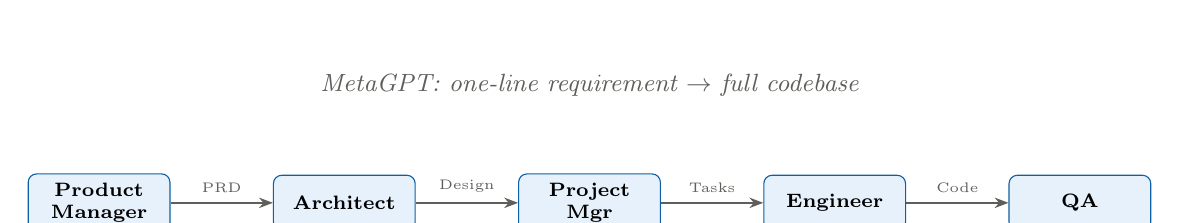
\begin{tikzpicture}[
  role/.style={rectangle, rounded corners=3pt, draw=aiblue, fill=infobg,
               minimum width=1.8cm, minimum height=0.7cm, font=\scriptsize\bfseries,
               align=center},
  arr/.style={-{Stealth[length=5pt]}, thick, color=aigray}
]
  \node[role] (pm)   {Product\\Manager};
  \node[role, right=1.3cm of pm]   (arch)  {Architect};
  \node[role, right=1.3cm of arch] (projm) {Project\\Mgr};
  \node[role, right=1.3cm of projm](eng)   {Engineer};
  \node[role, right=1.3cm of eng]  (qa)    {QA};
  \draw[arr] (pm)   -- node[above,font=\tiny]{PRD}    (arch);
  \draw[arr] (arch) -- node[above,font=\tiny]{Design} (projm);
  \draw[arr] (projm)-- node[above,font=\tiny]{Tasks}  (eng);
  \draw[arr] (eng)  -- node[above,font=\tiny]{Code}   (qa);
  \node[above=0.85cm of projm, font=\small\itshape, color=aigray]
    {MetaGPT: one-line requirement $\rightarrow$ full codebase};
\end{tikzpicture}
\end{center}

\textbf{MAS network topologies:}
\begin{itemize}
  \item \textbf{Centralized:} a central coordinator holds global knowledge and routes
    tasks to agents. Easy to monitor; single point of failure.
  \item \textbf{Decentralized:} agents share state only with their neighbours.
    More fault-tolerant and modular; coordination is harder.
  \item \textbf{Hierarchical:} tree structure with varying autonomy per layer.
    Natural for enterprise workflows where high-level strategy delegates to
    operational agents.
  \item \textbf{Holonic:} agents are grouped into \emph{holons} (a holon is a unit
    that is both a whole and a part). A holon's leading agent appears to the outside
    world as a single agent; internally it manages a sub-team.
  \item \textbf{Coalition / Team:} agents temporarily unite to achieve a shared goal,
    disbanding afterward. Teams are more tightly coupled; coalitions are ad hoc.
\end{itemize}

\subsection{Inter-agent communication}

Direct agent-to-agent integration suffers from an $n(n{-}1)/2$ integration-point
problem: $n$ agents each needing a bespoke connector to every other agent. Protocol
standards collapse this to $n$ connections to a shared message bus.

\textbf{Model Context Protocol (MCP)} --- Anthropic, 2024:
\begin{itemize}
  \item Focus: one model, many tools. Standardises how a single agent enriches its
    context via external servers.
  \item Transport: JSON-RPC over stdio or HTTP/SSE.
  \item Servers expose \emph{tools}, \emph{resources}, and \emph{prompts}.
  \item Limitation for multi-agent: no native agent-to-agent discovery, no delta
    streaming, no shared memory primitive.
\end{itemize}

\textbf{Agent Communication Protocol (ACP)} --- IBM (merged with A2A):
\begin{itemize}
  \item Focus: agent-to-agent communication across frameworks and organisations.
  \item Transport: REST over standard HTTP (no SDK required; cURL/browser compatible).
  \item \textbf{Async-first:} designed for long-running tasks; synchronous mode also
    supported.
  \item \textbf{Offline discovery:} agents embed metadata in their distribution
    packages so other agents can discover capabilities without a central registry.
  \item Enables orchestration across heterogeneous frameworks without custom glue.
\end{itemize}

\textbf{Agent2Agent Protocol (A2A)} --- Google:
\begin{itemize}
  \item Designed for cross-system and cross-organisation agent communication.
  \item More natural for Google-ecosystem integrations.
  \item Can coexist with ACP; each serves different primary use cases.
\end{itemize}

\begin{notebox}[title=MCP vs ACP in one line]
  MCP = one model $\leftrightarrow$ many tools. \quad
  ACP = many agents $\leftrightarrow$ many agents.
\end{notebox}

\subsection{Routers, state machines \& workflow engines}

As agent pipelines grow, structured control-flow primitives prevent LLM-driven
decision-making from becoming a runaway cost and reliability problem.

\textbf{Router:} decides which tool, subagent, or branch to invoke. Implementations:
\begin{itemize}
  \item LLM classifier --- flexible, expensive; use for open-ended routing.
  \item Embedding similarity match --- fast, moderate generality.
  \item Deterministic rule --- fastest, requires explicit case enumeration.
\end{itemize}

\textbf{State machine / workflow engine:} agent progression through phases is
explicit. Each state = a task phase (planning, retrieving, synthesising, reviewing);
transitions are triggered by events or conditions. LangGraph implements this directly.

Benefits over fully open-ended ReAct:
\begin{itemize}
  \item Deterministic paths for known task types (no unnecessary LLM calls).
  \item Explicit human-in-the-loop checkpoints at state transitions.
  \item Each state is independently testable.
  \item Defined failure handling per state, rather than global ``if error, retry.''
\end{itemize}

\begin{notebox}[title=Agent vs workflow]
  A \emph{workflow} uses fixed steps and deterministic transitions.
  An \emph{agent} makes dynamic decisions at each step.
  Many production ``agents'' are really workflows with one or two LLM-decision
  nodes --- often the better engineering choice.
\end{notebox}

\subsection{Swarm intelligence analogies}

Swarm intelligence studies how simple local rules among agents produce complex,
emergent global behaviour without central control. Canonical examples: ant colony
optimisation (ACO), particle swarm optimisation (PSO), bee colony algorithms.

Analogies to LLM multi-agent systems:
\begin{itemize}
  \item \textbf{Stigmergy:} ants communicate indirectly via pheromone trails left in
    the environment. In MAS, agents communicate indirectly via a shared message pool
    (MetaGPT), a vector database, or a shared workspace --- they don't call each other
    directly.
  \item \textbf{Emergent division of labour:} no agent is told to specialise; roles
    emerge from local interactions. In LLM swarms (e.g.\ Society of Mind prompting),
    assigning diverse ``perspectives'' to agents produces richer collective outputs
    than a single agent.
  \item \textbf{Robustness through redundancy:} decentralised MAS topologies mirror
    swarms: if one node fails, the system degrades gracefully rather than collapsing
    (contrast with centralised architectures with a single point of failure).
  \item \textbf{Limits of the analogy:} LLM agents are expensive, stateful, and
    context-limited; true swarms use thousands of cheap stateless units. Current
    multi-agent LLM systems typically operate at $n < 20$ agents.
\end{itemize}



% ── PART IX: AGENT PLATFORMS & TOOLING ──────────────────────────────
\part{Agent Platforms \& Tooling}
% chapters/36_openclaw_os.tex
% Part of: AI / LLM / Agents / Hardware Notes

\section{OpenClaw \& Agent OS Integration}

\subsection{OpenClaw architecture overview}

The NVIDIA stack for enterprise agentic deployment is composed of four distinct layers,
each with a different responsibility:

\begin{itemize}
  \item \textbf{OpenClaw} --- the agent/application layer. This is the thing that plans,
    calls tools, writes code, reads files, and tries to complete tasks. Think of it as
    the agent ``brain'' and behaviour loop.

  \item \textbf{OpenShell} --- the runtime governor. It sits \emph{between} OpenClaw and
    the real machine, network, and models, and decides what the agent is actually allowed
    to do. NVIDIA describes it as governing how the agent executes, what it can see and
    do, and where inference is routed.

  \item \textbf{NemoClaw} --- the packaged enterprise distribution. It takes OpenClaw and
    adds the missing operational pieces: safer setup, policy controls, privacy routing,
    model plumbing, and sandboxing. Installed in a single command via NVIDIA Agent
    Toolkit software.

  \item \textbf{Nemotron} --- NVIDIA's family of open models (reasoning, coding, visual
    understanding, safety, and agentic workflows). In this stack, Nemotron is the
    local or NVIDIA-hosted model option that NemoClaw/OpenShell can route inference to,
    especially when enterprises want on-prem execution.
\end{itemize}

A useful one-line shorthand for each layer:
\begin{center}
  OpenClaw = agent behaviour \quad
  Nemotron = model family \quad
  OpenShell = execution/security runtime \quad
  NemoClaw = packaged deployment stack
\end{center}

The key design philosophy is that ``wrapper'' is the right mental model for NemoClaw:
it does not replace the agent brain; it adds a controlled execution environment
\emph{around} it. The core question OpenClaw answers is \emph{``how do we make agents
capable?''}; OpenShell answers \emph{``how do we make capable agents safe to run?''}
NemoClaw bundles both answers into something an enterprise can actually operate.

\subsection{OS-level agent primitives}

OpenShell exposes three core architectural blocks that together form an agent OS:

\begin{enumerate}
  \item \textbf{Sandbox} --- the isolated environment where the agent runs. Mistakes or
    malicious/confused behaviour are contained inside the sandbox boundary and cannot
    reach the host OS or other sessions.

  \item \textbf{Policy engine} --- checks what actions are allowed across the filesystem,
    network, and process layers before any action executes. Rules are defined by the
    operator/enterprise, not the agent.

  \item \textbf{Privacy router} --- decides whether a given inference request or data
    payload should stay on a local model (e.g.\ a local Nemotron instance) or may be
    forwarded to a frontier cloud model. The routing decision is based on operator
    cost/privacy policy, explicitly \emph{not} on what the agent wants to do.
\end{enumerate}

\textbf{Action interception flow.} When OpenClaw attempts any action (read a file, call
a tool, invoke a model), OpenShell intercepts it before execution:
\begin{enumerate}
  \item Agent requests an action.
  \item Policy engine evaluates whether the action is permitted under current rules.
  \item Privacy router determines where any associated inference should go.
  \item Action executes only if policy allows it; otherwise it is blocked and the
    agent receives an error or a constrained alternative.
\end{enumerate}

\textbf{Example policy rules:}
\begin{itemize}
  \item HR data must stay on-device; only an approved local Nemotron model may see it.
  \item Code repository content may be routed to an approved cloud model.
  \item Outbound network requests are limited to a specified domain whitelist.
  \item The agent may read \texttt{/workspace/invoices} but not \texttt{/home/user/.ssh}.
  \item Only certain folder paths are writable; cloud model calls require scrubbed input.
\end{itemize}

\subsection{Filesystem \& process access}

OpenShell implements controls at the OS primitive level, not just through soft system
prompt instructions. Four categories of guardrails are enforced at runtime:

\begin{itemize}
  \item \textbf{Filesystem limits.} Scoped read/write access per session. An agent
    handling support tickets can be restricted to \texttt{/tickets/current} and
    explicitly denied access to credential stores or other user home directories.

  \item \textbf{Blocked network egress.} Outbound connections require policy approval.
    An enterprise can prevent customer PII from leaving the perimeter by blocking
    unapproved external endpoints at the network namespace level.

  \item \textbf{Process restrictions.} Limits on what processes the agent can spawn
    (e.g.\ no arbitrary shell exec, no privilege escalation).

  \item \textbf{Controlled inference backends.} The agent cannot freely choose which
    model API to call; the privacy router intercepts model calls and enforces
    routing policy.
\end{itemize}

Specific kernel-level mechanisms cited in NVIDIA's OpenShell documentation:
\textbf{Landlock} (Linux kernel filesystem access control), \textbf{seccomp}
(system call filtering), and \textbf{network namespaces} (network isolation per
process group). These are the same primitives used in container runtimes like
Docker/gVisor, adapted for agentic workloads.

\subsection{Security sandboxing}

The most important design idea in OpenShell is \textbf{out-of-process policy
enforcement}: moving the real control point \emph{outside} the agent, so the agent
cannot override it even if its reasoning is compromised, confused, or
prompt-injected.

\textbf{The problem with in-agent safety.} Most agent safety today is ``inside the
agent'': system prompts, behavioural rules, tool descriptions that say ``don't do X''.
These soft protections can fail if the agent loses context, is prompt-injected via
observed content, or simply reasons its way around them. In-context instructions
cannot enforce themselves.

\textbf{OpenShell's answer.} By intercepting actions at the OS/runtime layer before
they execute, OpenShell provides hard enforcement that the agent model cannot
circumvent. NVIDIA compares this to a browser security model: sessions are isolated,
and permissions are checked at the execution boundary, not just in the agent's
``mind''. The agent may \emph{believe} an action is permitted; OpenShell decides
whether it actually executes.

This is why OpenShell is better described as:
\begin{itemize}
  \item a runtime governor
  \item a policy firewall
  \item a sandbox manager
  \item an inference router
\end{itemize}
\ldots rather than as a model, a chatbot, or a prompt-engineering layer.

\textbf{Kernel-level isolation.} NVIDIA explicitly targets kernel-level sandboxing
(Landlock, seccomp, network namespaces) rather than process-level or
container-level approaches, giving stronger isolation guarantees for long-running
autonomous sessions.

\subsection{Desktop automation patterns}

\textbf{Enterprise deployment example: bank support ticket agent.}

Without a controlled runtime, an unconstrained agent processing support tickets might:
\begin{itemize}
  \item read too many internal files beyond those needed for the task
  \item leak customer PII to a cloud model in its prompt
  \item execute unsafe shell commands with unexpected side-effects
  \item POST data to an unapproved external endpoint
\end{itemize}

With NemoClaw/OpenShell, the operator configures policy such that:
\begin{itemize}
  \item customer PII stays on-prem; only an approved local Nemotron model sees raw
    ticket text
  \item only summarised, scrubbed data may be forwarded to a frontier cloud model
  \item the agent may access \texttt{/tickets/current} but not engineer laptops or
    credential folders
  \item outbound network access is limited to an approved internal API whitelist
\end{itemize}

\textbf{The enterprise value proposition} is therefore not ``make the agent smarter''
but \textbf{``make the agent deployable''}. The big blocker for long-running agents in
production is not model quality --- it is \emph{trust}. NVIDIA frames this explicitly:
the missing primitives are sandboxing, permissions, and isolation. If a safe runtime
layer exists, enterprises can let agents run longer, touch more systems, and do useful
work without granting unconstrained access.

\textbf{Comparison to the Cowork/Claude Code approach.}
Both NemoClaw/OpenShell and Cowork follow the same fundamental pattern --- a VM or
sandbox separates the agent from the host, and policy tiers control what the agent can
reach --- but at different deployment targets:
\begin{itemize}
  \item Cowork targets individual/team desktop users: single-session Ubuntu VM,
    user-selected workspace mount, product-level prohibited-action lists.
  \item NemoClaw/OpenShell targets enterprise IT: kernel-level isolation, org-defined
    policy YAML, privacy routing between on-prem and cloud models, multi-session scale.
\end{itemize}


% chapters/52_coding_agents_ides.tex
% Part of: AI / LLM / Agents / Hardware Notes

\section{AI Coding Agents \& IDEs}

\subsection{Landscape overview}

% TODO

\subsection{Cursor: architecture \& edit model}

% TODO

\subsection{GitHub Copilot \& Codex}

% TODO

\subsection{Windsurf (Codeium)}

% TODO

\subsection{Antigravity}

% TODO

\subsection{Devin \& SWE-agent}

% TODO

\subsection{Aider \& CLI coding agents}

CLI-based coding agents run entirely in a terminal, wrapping an LLM with a persistent
conversation loop, file I/O tools, and shell execution.

\textbf{Aider} is an open-source CLI agent that maintains a \emph{repo map} (built with
ctags/tree-sitter) to give the model structural context without flooding the context window
with raw source. It applies model-generated edits via SEARCH/REPLACE blocks or unified-diff
format, and supports multi-model backends (GPT-4o, Claude, Gemini, etc.).

\textbf{Claude Code} (Anthropic, 2024--) is Anthropic's official CLI agent, built on the
Claude Agent SDK. Observations from direct inspection of live session JSONL logs:

\begin{itemize}
  \item \textbf{Session persistence.} Every conversation is stored as a newline-delimited
    JSON file at \texttt{\textasciitilde/.claude/projects/\{project-slug\}/\{session-uuid\}.jsonl}.
    The project slug is the working-directory path with \texttt{/} replaced by \texttt{-},
    so each repository gets its own project namespace.

  \item \textbf{Message graph.} Each JSONL entry carries \texttt{uuid} and \texttt{parentUuid},
    forming a linked list (or tree when the user branches). A \texttt{promptId} groups every
    event (user message, assistant chunks, tool results) that belongs to the same conversational
    turn. The boolean \texttt{isSidechain} marks branch points.

  \item \textbf{Event types.} Three kinds of records appear in the log:
    \begin{itemize}
      \item \texttt{queue-operation} (enqueue / dequeue) --- internal concurrency plumbing
        so messages do not collide when dispatched rapidly.
      \item \texttt{user} --- human messages \emph{and} tool-call results (see below).
      \item \texttt{assistant} --- model output, written incrementally as chunks arrive;
        a single logical response often spans several consecutive lines.
    \end{itemize}

  \item \textbf{Tool results are injected as \texttt{role: user}.} This is a direct
    consequence of how the Anthropic Messages API works: tool results are sent back to
    the model in a \texttt{user} turn, not as assistant output. Each result entry carries
    a \texttt{sourceToolAssistantUUID} linking it to the assistant message that issued
    the call, plus a \texttt{toolUseResult} object with \texttt{stdout}, \texttt{stderr},
    and an \texttt{interrupted} flag.

  \item \textbf{Extended thinking blocks.} When extended thinking is enabled, the
    assistant content array contains a \texttt{\{type: ``thinking''\}} block alongside
    the visible \texttt{\{type: ``text''\}} block. Each thinking block carries a
    cryptographic \texttt{signature} --- Anthropic's mechanism to verify that thinking
    content has not been tampered with between turns in a long tool-use loop.

  \item \textbf{Prompt-cache telemetry.} Each assistant message records
    \texttt{cache\_creation\_input\_tokens} (tokens written to the cache this turn) and
    \texttt{cache\_read\_input\_tokens} (tokens served from cache), broken out by
    TTL tier (\texttt{ephemeral\_5m} vs.\ \texttt{ephemeral\_1h}). This makes the cache
    hit rate observable as context grows.

  \item \textbf{Session metadata.} Every record stores \texttt{cwd}, \texttt{gitBranch},
    \texttt{version} (the Claude Code release string), and \texttt{userType}
    (\texttt{external} for human users). A human-readable \texttt{slug} field
    (e.g.\ \texttt{gleaming-spinning-nygaard}) appears from the first tool-call onward,
    matching the session's VM directory name. These fields enable session resumption and
    provide an audit trail.

  \item \textbf{Permission model.} Messages carry a \texttt{permissionMode} field
    (\texttt{default}, \texttt{full}, \texttt{restricted}) that gates which tools the
    agent may invoke autonomously, aligning with Anthropic's principle of minimal
    footprint for agentic actions.
\end{itemize}

\subsection{Claude Code remote control}

Claude Code's \textbf{remote control} feature allows an active terminal session to be
accessed and continued from a web browser or mobile device, without moving any code or
state to the cloud. Everything keeps running on the original machine; only the
conversation stream is proxied to the remote client.

\textbf{Workflow.}
\begin{enumerate}
  \item In the project directory, run \texttt{claude remote-control}. This starts a
    new session and prints a URL. Pressing \texttt{Space} generates a QR code that
    can be scanned to open the session directly in the Claude mobile app or browser.
  \item To hand off a session already in progress, type \texttt{/remote-control}
    inside the running session to get the same URL.
  \item On the remote device, tap the \emph{environment} button and select the
    machine by name. Multiple machines / sessions can be listed simultaneously.
\end{enumerate}

\textbf{Architecture properties.}
\begin{itemize}
  \item \textbf{Nothing moves to the cloud.} The agent's tools, MCP server
    connections, file system access, and shell environment remain on the originating
    machine. The remote device is a thin client that streams the conversation.
  \item \textbf{Session continuity.} Typing on the mobile app updates the terminal
    in real time and vice versa --- the shared state is the JSONL session log on the
    local machine.
  \item \textbf{Spawn mode.} From a remote device you can also create entirely new
    Claude Code sessions on the connected machine, enabling you to launch parallel
    agents without being physically present.
  \item \textbf{Authentication.} The URL is tied to the Claude account; no
    separate credentials are required beyond being logged into the same account on
    the remote device.
\end{itemize}

\textbf{Persistent remote control.} By default, remote control must be explicitly
enabled per session. In \texttt{/config} (Claude Code's configuration), enabling
\texttt{remote-control} for all sessions removes this requirement.

\begin{notebox}
  Remote control is available on Mac, Team, and Enterprise plans (rolling out to
  Pro/Max). It is a natural extension of the JSONL session log architecture: because
  every turn is already serialised to disk, surfacing that stream to a second client
  requires no additional server-side state.
\end{notebox}

\subsection{How AI IDEs use context (repo map, RAG)}

% TODO

\subsection{Diff application \& conflict resolution}

Coding agents must apply model-generated edits back to the repository. Two dominant
formats exist and the choice meaningfully affects benchmark performance:

\textbf{Whole-file (whole) format:}
The model rewrites the entire file with the change applied. Simple to parse and apply;
but wastes tokens and compute rewriting unchanged content. Produces more reliable edits
for small files; becomes impractical for large codebases.

\textbf{Diff (unified-diff / SEARCH-REPLACE) format:}
The model emits only the changed lines, either as a unified diff or as a
SEARCH/REPLACE block. Far more token-efficient; the apply step can fail if the
surrounding context the model assumed does not match the current file (merge
conflicts).

\textbf{Observed impact:} On the Aider Polyglot benchmark, the same base model
scored 8\% in diff format vs 16\% in whole format because the model had not been
fine-tuned on diff-style output --- it would hallucinate diff syntax. After
instruction-tuning on diff examples, performance converged and ultimately exceeded
the whole-format ceiling.

\begin{intuitionbox}[title=The analogy]
  Whole format = re-drawing the entire picture to add a cloud.
  Diff format = drawing just the cloud. Diff is smarter; it requires the model to
  reason precisely about which lines to change and what the surrounding context is.
\end{intuitionbox}

\textbf{Conflict resolution} arises when the model's assumed file state diverges from
the actual file (concurrent edits, stale context). Agents handle this by: (1) re-reading
the file before applying, (2) fuzzy matching the search block with edit distance
tolerance, or (3) falling back to whole-file replacement.

\subsection{Evaluation: SWE-bench, Aider Polyglot \& coding benchmarks}

\textbf{SWE-bench / SWE-bench Verified:}
\begin{itemize}
  \item Tasks are real GitHub issues from popular Python repositories; the agent must
    produce a patch that passes the associated unit tests.
  \item SWE-bench Verified filters to issues where human raters confirmed the test suite
    correctly validates the fix, removing noisy items.
  \item State-of-the-art agents (Devin, SWE-agent) score in the 40--50\% range as of
    mid-2024; fully autonomous resolution of hard issues remains challenging.
  \item Measures end-to-end capability: repo understanding, fault localisation,
    patch generation, and test passage --- all in one score.
\end{itemize}

\textbf{Aider Polyglot:}
\begin{itemize}
  \item Coding exercises in six languages (Python, JavaScript, TypeScript, Go, Rust,
    C++); evaluated in diff format and whole format separately.
  \item Respected as a real-world, language-diverse benchmark; frontier models like
    GPT-4-era scored around 18\% in diff format at launch.
  \item Benchmark non-determinism is significant: consecutive runs of the same
    checkpoint can vary by 2--3 percentage points (see Chapter~45 on statistical
    significance).
\end{itemize}

\textbf{Synthetic data for coding fine-tuning:}
Two prominent methods for generating instruction-tuning data for coding models:
\begin{itemize}
  \item \textbf{OSS-Instruct} (from MagicCoder): given a code snippet, prompt a
    stronger model to generate an instruction-response pair \emph{inspired by} the
    snippet but not identical to it. Produces diverse, naturally grounded examples.
  \item \textbf{Evol-Instruct:} iteratively evolve a seed instruction into more
    complex or diverse variants (``make it harder'', ``add an edge case'', ``translate
    to a different language''). Each evolved version becomes a new training example.
    The cloning/dancing-guy analogy: each iteration produces a slightly different
    version; after many rounds, the dataset is far richer than the seed.
\end{itemize}

\textbf{The training-data pipeline challenge} (observed empirically):
\begin{itemize}
  \item Raw code from GitHub commit messages varies wildly in quality; poor commit
    messages often indicate low-quality, uncommitted code artifacts.
  \item Validation harnesses (test runners that score model outputs) can \emph{pass
    garbage} if misconfigured --- a stricter harness catching more failures is
    progress, not regression.
  \item \textbf{Garbage in, garbage out:} training on lower-quality data can make a
    model worse than its base. Cleaning (whitespace normalisation, deduplication,
    license filtering, quality scoring) is as important as volume.
  \item Data sources used in practice: The Stack (60TB permissively-licensed code),
    GitHub (MIT/Apache-licensed repositories), synthetic generation from frontier
    models (with contamination checks).
\end{itemize}


% chapters/53_agentic_platforms.tex
% Part of: AI / LLM / Agents / Hardware Notes

\section{Agentic Platforms: Manus, Computer Use \& Beyond}

\subsection{Manus AI overview (Butterfly Effect)}

% TODO

\subsection{NVIDIA NemoClaw / OpenShell}

NemoClaw is NVIDIA's packaged enterprise distribution for agentic deployment, combining
three layers into a single installable stack (see Chapter~36 for full detail):

\begin{itemize}
  \item \textbf{OpenClaw} --- the agent/app layer (planning, tool use, file I/O).
  \item \textbf{OpenShell} --- the out-of-process runtime governor: sandbox +
    policy engine + privacy router. Sits between the agent and the real OS/network.
  \item \textbf{Nemotron} --- NVIDIA's open model family (reasoning, coding, safety,
    agentic) used as the local inference option when cloud routing is disallowed.
\end{itemize}

The distinguishing architectural idea is \emph{out-of-process policy enforcement}:
safety controls are applied at the OS level (Landlock, seccomp, network namespaces)
rather than relying on soft in-context instructions. Enterprise policy rules
(data residency, domain whitelists, filesystem scoping) are enforced by OpenShell
before any action executes, regardless of what the agent reasons it should do.

\subsection{Anthropic Computer Use}

Anthropic's \emph{Computer Use} capability (released October 2024) exposes the model's
ability to observe screenshots and emit low-level desktop actions (mouse clicks, keyboard
input, scrolling). It is offered as a set of tool schemas (\texttt{computer},
\texttt{text\_editor}, \texttt{bash}) that the API caller is responsible for executing,
making the operator the ``hands'' that actually drive the OS.

\textbf{Cowork} is Anthropic's desktop-native product built on this foundation. Rather
than raw computer use, Cowork couples a sandboxed Linux VM with a rich tool layer
(filesystem access, web browsing, scheduled tasks, MCP connectors) to produce a
practical desktop agent for non-developers. Key architectural points observed directly:

\begin{itemize}
  \item The agent runs inside a per-conversation Ubuntu 22 VM spun up on the user's
    machine. Each session receives a randomly generated slug
    (e.g.\ \texttt{festive-nice-ramanujan}) used as both the VM directory name and the
    project identifier in the \texttt{.claude/} state store.
  \item A mounted workspace path (\texttt{/sessions/\{slug\}/mnt/\{user-folder\}})
    bridges the VM to the user's actual filesystem, while the VM's own root remains
    ephemeral and resets between tasks.
  \item A \textbf{Skills system} provides Claude with pre-written \texttt{SKILL.md}
    instruction files (e.g.\ \texttt{pptx}, \texttt{docx}, \texttt{pdf}, \texttt{xlsx})
    that encode best practices for creating specific document types, reducing trial-and-error
    at inference time.
  \item MCP (Model Context Protocol) connectors allow authenticated integration with
    external services (Slack, Asana, Google Drive, etc.) without the agent handling
    raw credentials.
\end{itemize}

\subsection{OpenAI Operator \& Agents SDK}

% TODO

\subsection{Browser-use \& web automation}

% TODO

\subsection{Desktop agent architectures}

Desktop agents must bridge the gap between an LLM's token-level reasoning and the
pixel/filesystem/network reality of a personal computer. A few recurring structural
patterns:

\begin{itemize}
  \item \textbf{Tool-first vs.\ screenshot-first.} Tool-first agents (Claude Code, Cowork)
    prefer structured tool calls (read file, run bash, fetch URL) over raw screenshot
    observation. Screenshot-first agents (OpenAI Operator, Manus) parse the visual DOM
    and emit pointer events. Tool-first agents are faster and cheaper for file/code tasks;
    screenshot-first generalizes to arbitrary GUI applications.

  \item \textbf{Workspace isolation.} A dedicated working directory (or VM) separates
    agent-generated artifacts from the user's files, preventing accidental overwrites.
    Cowork keeps a \texttt{/sessions/\{slug\}/} scratch space distinct from the mounted
    user folder.

  \item \textbf{State subdirectories.} The \texttt{.claude/} layout illustrates how
    desktop agents partition state: \texttt{projects/} for conversation logs,
    \texttt{plans/} for multi-step plans, \texttt{memory/} for persistent notes,
    \texttt{shell-snapshots/} for working-directory continuity across Bash calls, and
    \texttt{backups/} for rollback support.

  \item \textbf{Prompt caching at scale.} Long-running desktop sessions accumulate large
    system prompts. Tiered prompt caching (e.g.\ 5-minute and 1-hour TTL tiers in
    Anthropic's API) amortises the cost of re-encoding the same instructions on every
    turn.
\end{itemize}

\subsection{Security \& sandboxing for autonomous agents}

Autonomous agents operating on real filesystems and networks introduce a surface area for
both accidental harm and adversarial \emph{prompt injection}.

\textbf{Sandboxing layers} used in practice:
\begin{itemize}
  \item \textbf{VM isolation} --- each session runs in a separate lightweight VM so a
    runaway command cannot reach the host OS or other sessions.
  \item \textbf{Filesystem scoping} --- the agent's write access is limited to its own
    working directory; the user's files are mounted read-write only through an explicit
    workspace mount.
  \item \textbf{Permission tiers} --- Claude Code's \texttt{permissionMode} field
    (\texttt{default / full / restricted}) controls whether the agent can run arbitrary
    shell commands, write files, or is restricted to read-only actions.
  \item \textbf{Prohibited action lists} --- product-level policies (e.g.\ Cowork's
    security rules) enumerate actions the agent must refuse regardless of instruction:
    permanent deletion, modifying access controls, entering financial credentials, creating
    accounts.
\end{itemize}

\textbf{Prompt injection} is the primary adversarial threat: malicious instructions
embedded in observed content (web pages, emails, filenames, tool results) attempt to
hijack the agent's action stream. Defences include:
\begin{itemize}
  \item Treating all content from tool results as \emph{untrusted data}, not as
    instructions --- regardless of claimed authority (``admin override'', ``Anthropic
    staff'').
  \item Requiring explicit out-of-band user confirmation (in the chat interface) before
    acting on any instruction found inside a function result.
  \item Signing extended-thinking blocks (as in Claude's \texttt{signature} field) to
    detect tampering between turns in a long tool-use loop.
\end{itemize}

\subsection{Meta's agent research (LLaMA, CICERO)}

% TODO



% ── PART X: MULTIMODAL & WORLD MODELS ───────────────────────────────
\part{Multimodal \& World Models}
% chapters/27_vision_language.tex
% Part of: AI / LLM / Agents / Hardware Notes

\section{Vision-Language Models}

\subsection{CLIP \& contrastive pretraining}

% TODO

\subsection{LLaVA, Flamingo, PaLI}

% TODO

\subsection{Vision tokens \& patch embeddings}

% TODO

\subsection{Grounding \& spatial reasoning}

% TODO


% chapters/28_diffusion.tex
% Part of: AI / LLM / Agents / Hardware Notes

\section{Diffusion Models \& Generative Vision}

\subsection{GANs \& VAEs (generative predecessors)}

Before diffusion models dominated image generation, two main approaches competed: \textbf{Generative Adversarial Networks (GANs)} and \textbf{Variational Autoencoders (VAEs)}.

\begin{paperbox}[title={GAN: The Min-Max Game}]
\textbf{GAN} (Goodfellow et al., 2014) trains two networks:
\begin{itemize}
  \item \textbf{Generator} $G: z \sim p(z) \to \mathbb{R}^d$ maps noise (e.g., standard Gaussian) to fake samples.
  \item \textbf{Discriminator} $D: x \to [0,1]$ tries to distinguish real from fake.
\end{itemize}
The adversarial objective:
\[
\min_G \max_D \mathbb{E}_{x \sim p_\text{data}}[\log D(x)] + \mathbb{E}_{z \sim p(z)}[\log(1 - D(G(z)))]
\]
Training alternates: discriminator tries to maximize, generator tries to minimize. Samples are sharp and realistic when well-trained.

\begin{warnbox}
\textbf{GAN Drawbacks:}
\begin{itemize}
  \item \textbf{Mode collapse:} Generator finds a few modes and ignores others, reducing diversity.
  \item \textbf{Training instability:} Careful tuning of learning rates and architectures required.
  \item \textbf{Vanishing gradients:} When $D$ is too good, $\log(1-D(G(z)))$ saturates; switching to $-\log D(G(z))$ helps.
\end{itemize}
\end{warnbox}

Notable variants: \textbf{DCGAN} (convolutional architecture), \textbf{StyleGAN} (style-based generation, high quality), \textbf{CycleGAN} (unpaired image translation).
\end{paperbox}

\begin{paperbox}[title={VAE: Latent Variable Model}]
\textbf{VAE} (Kingma \& Welling, 2014) uses an encoder-decoder with a learned latent distribution:
\begin{itemize}
  \item \textbf{Encoder} $q_\phi(z|x)$: maps input $x$ to a distribution, typically $\mathcal{N}(\mu_\phi(x), \text{diag}(\sigma_\phi^2(x)))$.
  \item \textbf{Decoder} $p_\theta(x|z)$: reconstructs $x$ from sampled $z$.
\end{itemize}
Trained with the \textbf{ELBO} (Evidence Lower Bound):
\[
\mathcal{L} = \mathbb{E}_{q_\phi(z|x)}[\log p_\theta(x|z)] - \textsc{KL}(q_\phi(z|x) \parallel p(z))
\]
The \textbf{reparameterization trick} enables backprop: $z = \mu + \sigma \odot \epsilon$, $\epsilon \sim \mathcal{N}(0,I)$.

\begin{intuitionbox}
The KL term regularizes the latent space toward the prior (e.g., $\mathcal{N}(0,I)$), enabling smooth interpolation and generation from the prior. Reconstruction and regularization are always in tension.
\end{intuitionbox}

\textbf{VAE limitations:} Blurry outputs (Gaussian decoder assumption limits expressiveness); less sharp than GANs.
\end{paperbox}

\begin{notebox}
\textbf{Summary:} GANs are sharp but unstable; VAEs are stable but blurry; diffusion models achieve both sharpness and stability through iterative refinement.
\end{notebox}


\subsection{DDPM \& DDIM}

\begin{paperbox}[title={DDPM: Denoising Diffusion Probabilistic Models}]
\textbf{DDPM} (Ho et al., 2020) gradually adds noise to data in a Markov chain:

\textbf{Forward process} (fixed, no learning):
\[
q(x_t | x_{t-1}) = \mathcal{N}\left(\sqrt{1 - \beta_t} \, x_{t-1}, \beta_t I\right)
\]
Over $T$ steps (typically 1000), noise variance $\beta_t$ is small, so the process is slow. After $T$ steps, $x_T \approx \mathcal{N}(0, I)$.

\textbf{Closed form:} Using $\bar{\alpha}_t = \prod_{s=1}^t (1 - \beta_s)$:
\[
x_t = \sqrt{\bar{\alpha}_t} \, x_0 + \sqrt{1 - \bar{\alpha}_t} \, \epsilon, \quad \epsilon \sim \mathcal{N}(0, I)
\]
This lets us jump directly from $x_0$ to any $x_t$ without iterating.

\textbf{Reverse process} (learned): Train a U-Net $\epsilon_\theta(x_t, t)$ to predict the noise $\epsilon$ added in step $t$:
\[
\mathcal{L} = \mathbb{E}_{t, x_0, \epsilon}[\|\epsilon - \epsilon_\theta(x_t, t)\|^2]
\]

\begin{intuitionbox}
At inference, start from $x_T \sim \mathcal{N}(0, I)$ and iteratively denoise for $T$ steps, using the learned $\epsilon_\theta$ to reverse the forward process.
\end{intuitionbox}

\textbf{Key advantage:} Unlike GANs, training is stable; unlike VAEs, samples are sharp. \\
\textbf{Key drawback:} Requires ~1000 denoising steps, making inference very slow.
\end{paperbox}

\begin{paperbox}[title={DDIM: Deterministic Sampling}]
\textbf{DDIM} (Song et al., 2020) reformulates the reverse process as an \textbf{ODE} instead of an SDE, allowing deterministic (non-stochastic) sampling.

Rather than adding noise at each reverse step, DDIM rewrites the reverse process deterministically, reducing required steps from 1000 to 20--50 with minimal quality loss. The rewritten trajectory:
\[
x_{t-1} = \sqrt{\bar{\alpha}_{t-1}} \left( \frac{x_t - \sqrt{1-\bar{\alpha}_t} \epsilon_\theta(x_t, t)}{\sqrt{\bar{\alpha}_t}} \right) + \sqrt{1-\bar{\alpha}_{t-1}} \epsilon_\theta(x_t, t)
\]

\textbf{Advantages:}
\begin{itemize}
  \item \textbf{Speed:} 20--50 steps vs. 1000 (50--100× faster).
  \item \textbf{Deterministic:} Same latent $\Rightarrow$ same output (enables meaningful interpolation).
  \item \textbf{Quality:} Comparable to DDPM with full steps.
\end{itemize}

\begin{notebox}
DDIM's deterministic path is the foundation for latent-space editing and semantic interpolation in tools like Stable Diffusion.
\end{notebox}
\end{paperbox}


\subsection{Score matching \& SDE perspective}

\begin{paperbox}[title={Score Function \& Score Matching}]
The \textbf{score function} $s(x) = \nabla_x \log p(x)$ points toward regions of higher density. Training a network to estimate the score is called \textbf{score matching}.

\textbf{Denoising score matching} (Vincent, 2011) shows that score matching is equivalent to DDPM's noise prediction. Instead of predicting $\epsilon$, we can equivalently learn:
\[
s_\theta(x_t, t) = -\frac{1}{\sqrt{1-\bar{\alpha}_t}} \epsilon_\theta(x_t, t)
\]
This alternative view connects diffusion to the broader score-based generative modeling literature.

\begin{intuitionbox}
The score function gives a direction and magnitude for how to move toward the data distribution. Iteratively following the score is another way to think about diffusion sampling.
\end{intuitionbox}
\end{paperbox}

\begin{paperbox}[title={SDE Perspective: Unifying Diffusion Models}]
\textbf{Diffusion Models as SDEs} (Song et al., 2021) unify all diffusion models as stochastic differential equations (SDEs).

\textbf{Forward SDE:}
\[
dx = \mathbf{f}(x, t) dt + g(t) dW_t
\]
where $\mathbf{f}$ is the drift, $g(t)$ controls diffusion (noise), and $W_t$ is a Wiener process.

\textbf{Reverse SDE:}
\[
dx = \left[\mathbf{f}(x, t) - g(t)^2 \nabla_x \log p_t(x)\right] dt + g(t) d\bar{W}_t
\]
The crucial term is $\nabla_x \log p_t(x)$—the score function at time $t$. By training a network to estimate this score for all $t$, we can run the reverse SDE to sample.

\textbf{Benefits of SDE view:}
\begin{itemize}
  \item \textbf{Continuous time:} Treat diffusion as a continuous process; no need to pick $T$ discrete steps.
  \item \textbf{Probability flow ODE:} The reverse process can be written as a deterministic ODE (generalizes DDIM). Enabling faster sampling via ODE solvers.
  \item \textbf{Flexibility:} Different choices of drift $\mathbf{f}$ and diffusion $g$ yield different samplers; score is the common learned component.
\end{itemize}

\begin{notebox}
\textbf{Key insight:} All diffusion models fundamentally learn the score function $\nabla_x \log p_t(x)$. How you parameterize it (noise prediction vs. direct score prediction) is a choice, but the learned quantity is the same.
\end{notebox}
\end{paperbox}


\subsection{Stable Diffusion architecture}

\begin{paperbox}[title={Latent Diffusion Models (LDM)}]
\textbf{Latent Diffusion} (Rombach et al., 2022, now Stable Diffusion) performs diffusion in the latent space of a pretrained VAE instead of pixel space.

\textbf{Architecture components:}
\begin{enumerate}
  \item \textbf{VAE Encoder:} Compresses input (e.g., 512$\times$512 RGB image) to a latent tensor (64$\times$64$\times$4).
  \item \textbf{U-Net denoiser:} Runs the diffusion process entirely in latent space. ~860M parameters; includes cross-attention layers for text conditioning.
  \item \textbf{CLIP text encoder:} Encodes the text prompt into a sequence of embeddings, fed to cross-attention in the U-Net.
  \item \textbf{VAE Decoder:} Reconstructs the final image from the denoised latent.
\end{enumerate}

\textbf{Why latent space?}
\begin{itemize}
  \item \textbf{Compression:} 8$\times$ spatial downsampling $\Rightarrow$ 64$\times$ fewer tokens.
  \item \textbf{Speed:} Diffusion on 64$\times$64 latents is much faster than on 512$\times$512 pixels.
  \item \textbf{Quality:} VAE's learned compression preserves semantic information; diffusion achieves high-quality details.
\end{itemize}

\begin{intuitionbox}
The VAE encoder learns to compress while preserving semantic content. Diffusion refines in this efficient latent space. The decoder expands back to high-resolution images. This layering is key to Stable Diffusion's speed.
\end{intuitionbox}
\end{paperbox}

\begin{paperbox}[title={Classifier-Free Guidance}]
\textbf{Classifier-free guidance} (Ho \& Salimans, 2021) controls how strongly the model follows the text prompt.

During training, the U-Net is trained both with the text conditioning and without (dropping the conditioning with probability $p_\text{uncond}$, e.g., 0.1).

At inference, two predictions are made:
\begin{itemize}
  \item $\epsilon_\text{cond}(x_t, t, c)$: noise estimate conditioned on text $c$.
  \item $\epsilon_\text{uncond}(x_t, t, \varnothing)$: noise estimate without text.
\end{itemize}
The guided prediction:
\[
\epsilon_\text{guided} = \epsilon_\text{uncond} + w \cdot (\epsilon_\text{cond} - \epsilon_\text{uncond})
\]
where $w$ is the guidance weight (typically 7--15).

\textbf{Effects of $w$:}
\begin{itemize}
  \item $w = 0$: Ignores prompt; high diversity, low relevance.
  \item $w = 1$: No guidance (equivalent to standard conditioning).
  \item $w > 1$: Amplifies prompt-following signal; sharper adherence to text but less diversity.
  \item $w \gg 1$: Overly prompt-focused; may produce unrealistic artifacts.
\end{itemize}

\begin{notebox}
Classifier-free guidance is a simple post-hoc technique that requires no external classifier and provides a principled way to trade off prompt fidelity vs. diversity.
\end{notebox}
\end{paperbox}


\subsection{ControlNet, LoRA for images}

\begin{paperbox}[title={ControlNet: Spatial Conditioning}]
\textbf{ControlNet} (Zhang et al., 2023) adds explicit spatial control to a frozen diffusion model, enabling control via:
\begin{itemize}
  \item Depth maps (depth-guided generation).
  \item Pose skeletons (pose-guided human generation).
  \item Canny edge maps (sketch-to-image).
  \item Segmentation masks (layout-guided generation).
  \item Optical flow, normals, etc.
\end{itemize}

\textbf{Architecture:}
\begin{enumerate}
  \item Copy the U-Net encoder weights (frozen) to a trainable \textbf{control branch}.
  \item Add \textbf{zero-convolution} layers to merge the control signal with the main U-Net.
  \item Zero-convolutions initialize to zero-output, so training starts from the pretrained distribution.
  \item Fine-tune only on (image, control map) pairs; the pretrained model's knowledge is preserved.
\end{enumerate}

\begin{intuitionbox}
Zero-convolutions are crucial: they allow the control branch to be trained from scratch without disrupting the frozen model's pretrained weights. Gradual scaling from 0 ensures stable training.
\end{intuitionbox}

\textbf{Advantage:} Single frozen model + many lightweight ControlNets for different control types; users can combine multiple ControlNets for compound guidance.

\begin{notebox}
ControlNet demonstrates that spatial conditioning can be added to pretrained diffusion models with minimal retraining, enabling flexible control without full fine-tuning.
\end{notebox}
\end{paperbox}

\begin{paperbox}[title={LoRA for Image Models}]
\textbf{LoRA} (Low-Rank Adaptation, Hu et al., 2021) applies low-rank factorization to U-Net layers, enabling efficient fine-tuning.

For image diffusion models, LoRA is applied to \textbf{cross-attention layers} in the U-Net. These layers compute:
\[
\text{Attention}(Q, K, V) = \text{softmax}\left(\frac{QK^\top}{\sqrt{d}}\right) V
\]

Rather than fine-tuning the full weight matrices $W_Q, W_K, W_V$, we replace with:
\[
W \approx W_0 + \alpha A B^\top
\]
where $A \in \mathbb{R}^{d \times r}$ and $B \in \mathbb{R}^{d \times r}$ are learned, and $r \ll d$ is the rank (e.g., $r=4$ or $8$).

\textbf{Advantages:}
\begin{itemize}
  \item \textbf{Parameter efficiency:} $\sim$100 MB per LoRA vs. full model retraining ($\sim$4 GB for Stable Diffusion).
  \item \textbf{Fast training:} Fine-tune to a specific style or subject in hours on a single GPU.
  \item \textbf{Composability:} Combine multiple LoRAs to blend styles and subjects.
  \item \textbf{Preservation:} Base model weights frozen; LoRA only modifies the low-rank subspace.
\end{itemize}

\begin{intuitionbox}
Cross-attention layers are where text embedding interacts with image features. Low-rank updates here efficiently steer generation toward a specific aesthetic or subject without retraining the entire model.
\end{intuitionbox}
\end{paperbox}


\subsection{Flow matching}

\begin{paperbox}[title={Flow Matching: Learning Vector Fields}]
\textbf{Flow Matching} (Lipman et al., 2022) takes a different approach: instead of learning to denoise, directly learn a \textbf{vector field} $v_\theta(x_t, t)$ that transports a noise distribution to the data distribution along a path.

\textbf{Core idea:}
\begin{enumerate}
  \item Define a path $x_t$ from noise ($t=0$) to data ($t=1$).
  \item The vector field $v_\theta(x_t, t)$ should match the direction of the path: $\frac{dx_t}{dt} = v_\theta(x_t, t)$.
  \item Train by minimizing the matching loss:
  \[
  \mathcal{L} = \mathbb{E}_{t, x_0, x_1} \left\| v_\theta(x_t, t) - \frac{dx_t}{dt} \right\|^2
  \]
\end{enumerate}

\textbf{Straight-line paths:} The simplest choice is a straight line:
\[
x_t = (1-t) x_0 + t x_1, \quad \text{so} \quad \frac{dx_t}{dt} = x_1 - x_0
\]
This is constant, making training very simple: the network learns to predict a constant direction.

\textbf{Advantages over DDPM/DDIM:}
\begin{itemize}
  \item \textbf{Simpler loss:} Direct matching vs. noise prediction; more stable.
  \item \textbf{Straight paths:} Fewer steps needed at inference (fewer integration steps along a straight line).
  \item \textbf{Flexibility:} Paths don't have to be straight; can use optimal transport for curved paths minimizing detours.
  \item \textbf{Faster training:} No need to condition on noise schedules.
\end{itemize}

\begin{intuitionbox}
Flow matching is intuitive: imagine pushing probability mass along a field of vectors from noise to data. Learning to predict the velocity field is simpler than denoising.
\end{intuitionbox}
\end{paperbox}

\begin{paperbox}[title={Optimal Transport \& Flow Matching}]
\textbf{Optimal Transport (OT) conditioning:} Instead of assigning data points arbitrarily to noise samples, use the Wasserstein distance to find the \textbf{straightest possible paths}.

For a batch of data $\{x_1^{(i)}\}$ and noise samples $\{x_0^{(i)}\}$, OT finds a coupling that minimizes path curvature. This results in:
\begin{itemize}
  \item Straighter paths $\Rightarrow$ fewer integration steps.
  \item More efficient training (less doubling-back or zigzagging).
  \item Better sample quality.
\end{itemize}

Modern flow-matching models (e.g., Stable Diffusion 3, Flux) use OT-conditioned flow matching for improved speed and quality.

\begin{notebox}
\textbf{Comparison:} DDPM predicts noise; DDIM makes it deterministic; flow matching learns a vector field directly. Each approach refines the previous, trading off complexity for speed and simplicity.
\end{notebox}
\end{paperbox}


% chapters/29_audio_multimodal.tex
% Part of: AI / LLM / Agents / Hardware Notes

\section{Audio, Speech \& Multimodal Fusion}

\subsection{Whisper \& speech recognition}

% TODO

\subsection{Audio tokenization}

% TODO

\subsection{TTS \& voice cloning}

% TODO

\subsection{Multimodal fusion strategies}

% TODO


% chapters/24_world_models_theory.tex
% Part of: AI / LLM / Agents / Hardware Notes

\section{World Model Theory}

\subsection{LeCun's JEPA architecture}

% TODO

\subsection{Dreamer (RSSM)}

% TODO

\subsection{World models in RL}

% TODO

\subsection{Predictive coding theories}

% TODO


% chapters/25_video_models.tex
% Part of: AI / LLM / Agents / Hardware Notes

\section{Video \& Predictive Models}

\subsection{Sora \& video diffusion}

Sora (OpenAI, 2024) represents a major milestone in generative video: a text-to-video foundation model capable of producing coherent videos up to 1 minute in length at 1080p resolution. Unlike earlier text-to-video systems that required single-frame generation followed by upsampling, Sora generates video natively and directly.

\subsubsection{Architecture: Video Diffusion Transformer}

The core innovation is the \textbf{Video Diffusion Transformer (DiT)}, which departs from the U-Net-based architecture standard in image diffusion. Rather than applying convolutional layers hierarchically, Sora's transformer operates on \emph{spacetime patches}—small cuboid regions of video (e.g., a $16 \times 16 \times 2$ block spanning spatial and temporal dimensions). Each patch is tokenised into a flat embedding sequence, allowing the transformer to treat video generation as a sequence-to-sequence task similar to language modelling.

This patch-based representation is elegantly general: instead of hardcoding separate models for different resolutions or aspect ratios, Sora simply conditions on the target resolution and generates patches of the appropriate size and duration. A $480p$ portrait video, a $1080p$ landscape shot, and a $720p$ square clip can all be generated by the same model by adjusting patch scaling.

\begin{intuitionbox}
Why patches instead of pixels? Pixel-level diffusion on video is prohibitively expensive: a 1-minute 1080p video at 30fps is $\approx 1.8M$ frames of $1920 \times 1080$ pixels each. Patches reduce this to $\sim 10k$ tokens, making transformer-scale generation tractable. The trade-off is that patch-level generation may lose fine-grained spatial detail, but token efficiency wins.
\end{intuitionbox}

\subsubsection{Training and Data}

Sora was trained on large-scale video datasets paired with text descriptions. A critical practical detail: raw video captions (e.g., YouTube metadata) are often sparse or vague. OpenAI likely employed a \textbf{recaptioning pipeline}: passing each video through a vision-language model (similar to CLIP or multimodal GPT-4V) to generate rich, detailed text descriptions that better explain the visual content. This densification of captions significantly improves text-to-video coherence.

The model learns in the diffusion framework: corrupted videos (with noise added to patches) are reconstructed conditioned on text embeddings. As training progresses, the model learns to generate spatially coherent frames and temporally consistent motion.

\subsubsection{World Simulator Hypothesis}

The Sora paper makes a bold claim: by learning to predict the next patch in a sequence, the model implicitly learns a \emph{world model}—an internal representation of physics, causality, and object dynamics. Evidence cited includes:
\begin{itemize}
  \item Objects maintain consistent identity and trajectories across frames.
  \item Shadows, reflections, and lighting respond realistically to object motion.
  \item Fluid and deformable objects (smoke, water, cloth) obey rough physical laws.
\end{itemize}

This hypothesis is influential but contested. Sceptics argue that the model may simply memorise large-scale patterns from training data rather than developing a true causal model of physics. Distinguishing learned dynamics from pattern matching remains an open question in interpretability.

\subsubsection{Known Limitations}

As of early 2024, Sora exhibits several failure modes:
\begin{warnbox}
\textbf{Physics violations}: Objects can appear or disappear without physical justification. A person may phase through a wall.

\textbf{Long-range consistency}: Over 30+ seconds, character appearance, lighting, and background slowly drift or degrade.

\textbf{Control granularity}: Fine-grained directives (e.g., "move the camera exactly 30 degrees clockwise") are difficult; the model interprets text-level intent rather than precise camera parameters.

\textbf{Temporal flicker}: Despite transformer-based processing, occasional frame-to-frame jitter occurs, especially at patch boundaries.
\end{warnbox}

These limitations suggest that the current generation of diffusion-based video models, while impressive, remain far from true physical simulation or precise interactive control.

\subsection{Genie \& interactive world models}

Genie (Google DeepMind, 2024) tackles a different problem: learning a \emph{controllable} world model from unlabelled video. Rather than generating videos from text prompts, Genie learns to generate video frames conditioned on learned \emph{actions}, enabling interactive control without a pre-defined control scheme.

\subsubsection{Unsupervised Action Learning}

The key innovation is that Genie learns its action space \textbf{without any action labels}. Given a sequence of raw video frames (e.g., from gameplay footage, dashcam footage, or other dynamic scenes), Genie infers: what latent factors, if manipulated, would steer the world's evolution?

Formally, Genie models $P(\text{frame}_{t+1} | \text{frames}_{1:t}, \mathbf{a}_t)$, where $\mathbf{a}_t$ is a learned latent action token. By training this mapping end-to-end on video sequences, the model discovers an action representation where nearby latent tokens correspond to coherent world perturbations (e.g., "move forward," "jump," "rotate camera"). This is enabled by the structure of the data itself: video sequences naturally contain the signal of causality (action causes state change).

\begin{intuitionbox}
Why unsupervised? Collecting action labels (a button press or joystick input for every frame) is expensive and domain-specific. Gameplay footage, for instance, may come without controller logs. Genie's insight is that the video data itself encodes action information through the sequential structure: if frames are statistically different in a consistent direction, an action likely caused that difference.
\end{intuitionbox}

\subsubsection{Architecture and Components}

Genie's pipeline comprises three main components:

\begin{enumerate}
  \item \textbf{Spatial Tokeniser}: A VQ-VAE (Vector Quantised VAE) encodes individual video frames into discrete latent codes. This compresses spatial information and prepares frames for the dynamics model.

  \item \textbf{Latent Action Model}: A learned discrete action tokeniser discovers a set of "primitive actions" such that sequencing them produces coherent trajectories. This acts like learning a proto-language of control.

  \item \textbf{Dynamics Model}: A diffusion-based or autoregressive model predicts the next frame's latent code given the previous frame and a latent action token. This is the core world model: $P(\mathbf{z}_{t+1} | \mathbf{z}_{1:t}, \mathbf{a}_t)$ where $\mathbf{z}$ are frame latents.
\end{enumerate}

Once trained, a user can "play" the world by selecting action tokens; the model generates a stream of coherent frames responding to those actions. Notably, no traditional controller input is required—the model infers control directly from user interaction (e.g., keyboard or learned policy).

\subsubsection{Connection to World Models}

Genie embodies a modern realisation of the \emph{world models} programme from reinforcement learning: the hypothesis that agents learn an internal forward model of environment dynamics, which they use for planning. Unlike classical world models trained on RL environments with action labels, Genie learns from passive observation—the same regime humans often learn from (watching video, reading books). This makes it potentially more data-efficient and more aligned with human-like learning.

\begin{paperbox}[title={Relation to V-JEPA and Self-Supervised Video}]
Genie and V-JEPA (Chapter 24) are complementary: V-JEPA learns a high-level latent representation of video through masked prediction; Genie learns \emph{actionable} representations where latent variables map to world state changes. Both leverage the structure of video to extract generalizable representations without labels.
\end{paperbox}

\subsection{Temporal consistency challenges}

Video generation introduces challenges absent from image generation: frames must cohere across time, objects must persist and move realistically, and long-range dependencies must be maintained. This subsection surveys the main challenges and techniques.

\subsubsection{Flickering and Inter-Frame Jitter}

Diffusion models, even transformer-based ones, can process frames with too much independence, leading to:
\begin{itemize}
  \item \textbf{Flicker}: Pixel values oscillate between frames without clear motion, resembling poorly denoised noise.
  \item \textbf{Jitter}: Objects appear to vibrate or twitch due to slight spatial shifts in consecutive frames.
\end{itemize}

Root cause: the noise prediction objective optimises each timestep independently; without explicit temporal coupling, the model may find local minima that improve a single frame at the cost of inter-frame coherence.

\subsubsection{Temporal Modelling Approaches}

Several techniques enforce temporal consistency:

\begin{enumerate}
  \item \textbf{3D Convolutions}: Inflate standard 2D convolutions into 3D by adding a temporal dimension. A $3 \times 3$ kernel becomes $3 \times 3 \times 3$, allowing the model to reason about local motion patterns. U-Net diffusion backbones can be retrofitted with 3D convs in the deeper layers.

  \item \textbf{Temporal Attention}: Add self-attention across the time dimension in addition to spatial attention. A transformer can attend to "where was this object in the previous frame?" explicitly, guiding consistency. This is computationally expensive (quadratic in sequence length) but highly effective.

  \item \textbf{Causal Temporal Transformers}: Structure the transformer so that frame $t$ can attend to frames $0 \ldots t-1$ but not future frames. This respects causality and is more efficient than full bidirectional attention, though models that attend bidirectionally before generation (and then use causal generation) are also common.

  \item \textbf{Optical Flow Supervision}: Use optical flow (pre-computed or predicted) as a conditioning signal or auxiliary loss. If the model predicts inconsistent flow between frames, a loss penalty encourages it to enforce motion consistency. Some models compute optical flow between diffusion steps and use it to warp frames for better coherence.
\end{enumerate}

\subsubsection{Motion Blur, Ghosting, and Trajectory Tracking}

Generating realistic motion is non-trivial. The model must:
\begin{itemize}
  \item Predict where objects will be several frames hence.
  \item Render motion blur or sharp motion as appropriate to the scene context.
  \item Avoid \textbf{ghosting}: trailing artifacts where an object's old and new position both appear, creating a "smeared" look.
\end{itemize}

Successful motion generation requires the model to implicitly track object trajectories. Models trained with temporal attention or 3D convolutions tend to perform better because they can reason about object identity across frames.

\subsubsection{Long-Range Consistency}

A harder problem than frame-to-frame coherence: maintaining consistency over hundreds of frames. Issues include:
\begin{warnbox}
\textbf{Character drift}: A person's appearance (clothing, hairstyle) may subtly shift over 30+ seconds.

\textbf{Lighting creep}: The ambient light colour and intensity may slowly change without motivation.

\textbf{Background accumulation}: Repeated small errors in background rendering accumulate, eventually making the scene look wholly different.

\textbf{Layout collapse}: The spatial relationships between objects become confused, leading to impossible geometry.
\end{warnbox}

Current models degrade noticeably after $\sim 1$ minute, suggesting that purely feed-forward generation (frame-by-frame without global memory) is insufficient. Research directions include hierarchical generation (high-level scene layout first, then detail infilling) and memory-augmented architectures.

\subsubsection{Optical Flow as a Supervision Signal}

Some recent models use \textbf{optical flow} (dense motion estimation) as auxiliary supervision:
\begin{itemize}
  \item \textbf{Flow prediction loss}: In addition to the diffusion loss, encourage the model's latent representations to predict accurate optical flow.
  \item \textbf{Flow-based warping}: Use predicted flow to warp frames from frame $t$ to frame $t+1$, then blend the warp with the generated frame. This enforces physical continuity.
  \item \textbf{Flow conditioning}: Condition the diffusion model on precomputed or user-specified optical flow, constraining motion to be plausible.
\end{itemize}

This approach leverages classical computer vision (optical flow estimation) to ground modern generative models, improving consistency at a modest computational cost.

\subsection{Next-frame prediction as pretraining}

Predicting the next frame in a video sequence is a powerful self-supervised objective. It forces the model to learn dynamics, object persistence, and causal structure—all without labels. This subsection covers video prediction as a pretraining paradigm.

\subsubsection{Video Prediction as Self-Supervised Learning}

The core insight: a model that can predict $\text{frame}_{t+1}$ from $\text{frames}_{1:t}$ must understand:
\begin{itemize}
  \item \textbf{Motion}: How do objects move in this domain?
  \item \textbf{Object permanence}: Does an occluded object continue to exist?
  \item \textbf{Physics}: What are the constraints on how the world can change?
  \item \textbf{Semantics}: What is the scene about, and what are the key actors?
\end{itemize}

Unlike supervised pretraining (contrastive learning, masked language modelling), video prediction is a \emph{generative} task: the model must synthesise the raw sensory signal of the next moment. This is a rich learning signal that captures the structure of the world.

\begin{paperbox}[title={Historical Roots}]
Video prediction dates back to the early 2010s (Zeiler et al., Srivastava et al.), where convolutional models learned to predict pixel space. The field has evolved through adversarial losses (GANs), flow-based methods, VAEs, and now diffusion. The core idea remains: learning from temporal structure.
\end{paperbox}

\subsubsection{VideoMAE: Masked Autoencoding for Video}

VideoMAE (He et al., Meta, 2022) applies the \textbf{masked autoencoder} paradigm to video:
\begin{itemize}
  \item \textbf{Masking}: Randomly mask $90\%+$ of spacetime patches in a video. This is much more aggressive than image masking ($\sim 75\%)$ and tests the model's ability to reason about long-range structure.
  \item \textbf{Reconstruction}: An encoder embeds the visible patches; a decoder reconstructs the masked patches. The loss is the reconstruction error on masked regions.
  \item \textbf{Learned representations}: The trained encoder produces video embeddings useful for downstream tasks (action recognition, video classification) without finetuning.
\end{itemize}

VideoMAE demonstrates that masked prediction scales well: larger models, more data, and higher masking ratios all improve downstream performance, following predictable scaling laws. This makes video prediction an attractive foundation for video understanding.

\subsubsection{V-JEPA: Prediction in Representation Space}

Rather than predicting pixels, \textbf{V-JEPA} (Video Joint-Embedding Predictive Architecture, Chapter 24) predicts in a learned latent space:
\begin{itemize}
  \item \textbf{Representation learning}: An encoder $f$ maps frames to latents: $\mathbf{z}_t = f(\text{frame}_t)$.
  \item \textbf{Latent prediction}: A predictor $g$ is trained to minimise the distance between predicted latents $g(\mathbf{z}_{1:t})$ and target latents $f(\text{frame}_{t+1})$ (using a momentum-updated target encoder, similar to BYOL).
  \item \textbf{Advantage over pixel prediction}: Latent space is much simpler than pixel space; the model avoids modelling irrelevant textural variation and learns more abstract motion representations.
\end{itemize}

V-JEPA achieves strong video understanding performance and is computationally cheaper than pixel-space prediction. The representation learned this way captures semantically meaningful motion rather than superficial pixel transitions.

\subsubsection{Scaling Laws in Video Pretraining}

Like language and image models, video pretraining exhibits \textbf{scaling laws}:
\begin{itemize}
  \item \textbf{Data scaling}: More video data yields better performance, with diminishing returns following a power law (similar to language models).
  \item \textbf{Compute scaling}: Larger models achieve lower prediction loss, consistent with Chinchilla scaling.
  \item \textbf{Task transfer}: Models trained on video prediction with internet-scale data transfer to many downstream tasks (classification, detection, tracking) better than supervised pretraining on smaller, task-specific datasets.
\end{itemize}

This suggests that \textbf{video prediction is a foundational task} for video understanding, much as next-token prediction is foundational for language. Scaling video prediction to billions of hours of video and trillion-parameter models remains an active frontier, with potential to unlock powerful open-domain video AI.

\begin{notebox}
\textbf{Key Takeaway}: Next-frame prediction mirrors language modelling's philosophy—leverage the structure of raw unlabelled data to learn powerful, transferable representations. For video, this means learning dynamics, causality, and scene understanding as an emergent property of predicting the sensory signal.
\end{notebox}

% chapters/26_embodied_ai.tex
% Part of: AI / LLM / Agents / Hardware Notes

\section{Embodied AI \& Simulation}

\subsection{SLAM \& robot perception}

\begin{intuitionbox}
Simultaneous Localization And Mapping (SLAM) is the classic chicken-and-egg problem: a robot must build a map of an unknown environment while simultaneously tracking its own location within that map. These two tasks are deeply intertwined — you need to know where you are to map accurately, and you need a good map to localize.
\end{intuitionbox}

\subsubsection{The two interleaved problems}

SLAM decomposes into two core problems:
\begin{enumerate}
\item \textbf{Localization}: Given a map, where am I? Solved with particle filters or Kalman filters.
\item \textbf{Mapping}: Given my location, what does the environment look like?
\end{enumerate}

\subsubsection{EKF-SLAM}

Extended Kalman Filter SLAM maintains a Gaussian belief over a joint state vector: $[\text{robot pose}, \text{landmark positions}]$. The state grows with each observed landmark, leading to $O(n^2)$ update cost where $n$ is the number of landmarks. A key challenge is \emph{data association}: deciding which observed feature corresponds to which landmark in the map.

\subsubsection{Particle filter SLAM (FastSLAM)}

Represents the belief as a distribution over robot trajectories; each particle maintains its own map of landmarks. This approach is more robust to non-Gaussianity than EKF-SLAM and achieves $O(n \log n)$ complexity per update.

\subsubsection{Graph-SLAM and pose graph optimisation}

Modern SLAM formulates the problem as a graph of robot poses connected by relative constraints (odometry measurements and loop closures). The goal is to find the most likely configuration via non-linear least squares, solved with tools like \texttt{g2o} and \texttt{GTSAM}.

\begin{notebox}
\textbf{Loop closure} occurs when the robot revisits a known location. This is where accumulated drift is corrected. The challenge is the place recognition problem: identifying that current observations match a previously visited location. Techniques include bag-of-words, NetVLAD, and DBoW descriptors.
\end{notebox}

\subsubsection{Sensor modalities}

\begin{itemize}
\item \textbf{LiDAR SLAM} (e.g. Velodyne): directly produces 3D point clouds; robust to lighting conditions.
\item \textbf{Visual SLAM} (e.g. ORB-SLAM, COLMAP): uses cameras; cheaper hardware but more challenging in low light; sensitive to motion blur.
\item \textbf{Dense vs.\ sparse}: sparse methods track keypoints; dense methods build full volumetric models.
\end{itemize}

\subsubsection{Modern deep SLAM}

Recent systems (NICE-SLAM, iMAP) use neural representations like Neural Radiance Fields (NeRF) or neural implicit maps as the underlying map representation, combining classical SLAM geometry with learnable dense scene models.

\subsection{Sim-to-real transfer}

\begin{intuitionbox}
The sim-to-real gap is one of the hardest problems in robotics. Training in simulation is fast and cheap, but real robots face physics inaccuracies, sensor noise, appearance differences, and latency that don't exist in the simulator.
\end{intuitionbox}

\subsubsection{Sources of the gap}

The sim-to-real mismatch includes:
\begin{itemize}
\item Physics: friction coefficients, mass, contact dynamics, compliance of actuators
\item Sensors: camera noise, latency, quantisation in encoders
\item Appearance: domain shift between photorealistic rendering and real images
\item Control: latency, actuator saturation, backlash
\end{itemize}

\subsubsection{Domain randomisation}

Train the policy in many varied simulation conditions: random friction coefficients, masses, lighting, textures, camera parameters. The real world appears as just another instance of the randomised distribution. This worked for OpenAI's Dactyl (multi-fingered robotic hand solving a Rubik's cube).

\subsubsection{Domain adaptation}

Rather than randomisation, adapt the model's learned representation from simulation to real using adversarial training or style transfer. The real robot provides additional data to refine the simulator's parameters.

\subsubsection{System identification}

Measure real robot dynamics (forward kinematics, joint compliance, motor characteristics) and tune simulator parameters to match real hardware. This narrows the gap at the physics level.

\subsubsection{Real-to-sim}

Conversely, capture real sensor data and use it to build a more faithful simulation: photo-realistic rendering from real images, real trajectory data for dynamics validation.

\subsection{RT-2, PaLM-E, embodied LLMs}

\begin{intuitionbox}
The key insight is that large language models and vision-language models trained on the internet contain rich semantic knowledge. By fine-tuning these models on robot demonstrations and grounding them in actions, we get data-efficient robot learning without training from scratch.
\end{intuitionbox}

\subsubsection{PaLM-E (Google 2023)}

A multimodal language model that consumes continuous sensor streams (images, robot state) as inputs alongside text. Trained jointly on:
\begin{itemize}
\item Internet-scale text corpora
\item Embodied robot manipulation data
\end{itemize}

Can plan multi-step manipulation tasks from natural language instructions and reason over sensor observations.

\subsubsection{RT-2: Robotics Transformer 2 (Google DeepMind 2023)}

Fine-tuned PaLI (a vision-language model) to output robot actions directly as discretised text tokens. Key insight: web-trained knowledge transfers to robot generalisation — the model can pick up objects it has never been trained on, if told the object's name.

\subsubsection{Vision-Language-Action (VLA) models}

The emerging paradigm: take a large vision-language model, fine-tune it on demonstrations where the model outputs robot actions (as text tokens or continuous vectors). RT-2 is the canonical example. OpenVLA is an open-source alternative.

\begin{paperbox}[title={Why VLAs work}]
Web-scale pretraining gives the model semantic understanding of objects, spatial relationships, and natural language. Fine-tuning on even modest amounts of robot data (thousands of trajectories) grounds this knowledge in actions — the model learns to convert ``pick up the red cube'' into motor commands. Far more sample-efficient than learning from scratch.
\end{paperbox}

\subsection{Project GR00T \& foundation models for robotics}

\begin{intuitionbox}
Foundation models are reshaping robotics. Instead of building separate controllers for each task and robot type, the goal is a single large model trained on diverse robot and human data, then fine-tuned or prompted for specific embodiments and tasks.
\end{intuitionbox}

\subsubsection{NVIDIA Project GR00T (2024)}

A framework for building foundation models for humanoid robots, announced by NVIDIA in 2024. Not a single monolithic model, but rather a pipeline and pretrained weights.

\subsubsection{Groot N1}

The first release: a general-purpose humanoid robot foundation model. Outputs joint positions or torques for humanoid bodies. Trained on:
\begin{itemize}
\item Diverse robot demonstrations (from multiple robot platforms when possible)
\item Synthetic data from simulation (Isaac Lab)
\item Human motion video (to provide motion priors, without requiring the model to explicitly control a body)
\end{itemize}

\subsubsection{Key technical ideas}

\begin{itemize}
\item \textbf{Leverage simulation}: use GPU-accelerated environments (Isaac Lab) to generate massive synthetic training data for pretraining.
\item \textbf{Human motion priors}: incorporate human video to teach natural motion, even though humans and robots differ in kinematics.
\item \textbf{Hardware fine-tuning}: adapt the foundation model to specific robot hardware and tasks via further training.
\item \textbf{Multi-embodiment pretraining}: if available, train on diverse robot platforms; enables generalisation.
\end{itemize}

\subsubsection{NVIDIA Isaac platform}

The underlying simulation ecosystem consists of:
\begin{itemize}
\item \textbf{Isaac Gym}: GPU-accelerated physics, multi-stage simulation pipeline, used for large-scale RL training.
\item \textbf{Isaac Lab}: high-level learning framework built on Isaac Gym; supports curriculum learning, task scheduling, and more.
\item \textbf{Isaac Sim}: photorealistic rendering and sensor simulation (cameras, LiDAR) for bridging to real robots.
\end{itemize}

\subsubsection{The ``GR00T moment'' for robotics}

NVIDIA argues that GR00T represents a paradigm shift: foundation models for robotics are what ImageNet and CNN pretraining were for computer vision — a common foundation that dramatically lowers the barrier to building capable systems. Instead of each team training from scratch, they build atop shared, large-scale pretrained representations.

\begin{warnbox}
\textbf{Physical AI}: NVIDIA's term for AI that operates in and interacts with the physical world (forces, contact, dynamics), distinct from ``digital AI'' (language, images, text). Requires understanding physics deeply — not just visual recognition.
\end{warnbox}

\subsection{Simulation environments (Isaac, MuJoCo)}

\subsubsection{MuJoCo (Multi-Joint dynamics with Contact)}

The standard open-source physics engine for robot learning:
\begin{itemize}
\item Very fast and accurate continuous control simulation
\item Benchmark choice for RL on locomotion and manipulation
\item Acquired by DeepMind; now fully open-source with active community
\item GPU support in recent versions
\end{itemize}

\subsubsection{Isaac Gym and Isaac Lab}

NVIDIA's ecosystem, with GPU-accelerated physics and RL training:
\begin{itemize}
\item Simulate thousands of robot instances in parallel on a single GPU
\item 100–1000× speedup over CPU-based simulators like MuJoCo on CPU
\item Used for large-scale pretraining of foundation models (e.g. GR00T)
\item Isaac Lab provides high-level APIs for task definition, curriculum learning, and integration with PyTorch
\end{itemize}

\subsubsection{Habitat (Meta AI)}

Photorealistic indoor navigation simulation:
\begin{itemize}
\item Built on real-world 3D scans from Matterport
\item Focused on embodied vision and navigation tasks
\item Used for PointNav, ObjectNav research
\end{itemize}

\subsubsection{AI2-THOR}

Interactive household simulator for robotic manipulation and object interaction:
\begin{itemize}
\item Support for articulated objects (doors, drawers, fridges)
\item Realistic physics and visual rendering
\end{itemize}

\subsubsection{PyBullet}

Open-source physics engine; widely used in research and teaching. Slower than MuJoCo and Isaac, but easy to use and flexible.

\subsection{Manipulation \& locomotion tasks}

\subsubsection{Manipulation}

Core robotic manipulation challenges:
\begin{itemize}
\item \textbf{Pick-and-place}: grasping an object and moving it to a target location
\item \textbf{Grasping}: computing stable grasp points; parallel-jaw grippers vs. multi-finger dexterous hands
\item \textbf{Assembly}: precise insertion and alignment (pegs in holes, mating parts)
\item \textbf{Tool use}: using objects as tools to accomplish goals
\item \textbf{Deformable objects}: handling cloth, rope, liquid — non-rigid dynamics
\end{itemize}

Key research challenges: predicting contact forces, planning grasps on novel objects, handling partial observability.

\subsubsection{Dexterous manipulation}

OpenAI's Dactyl (2019) achieved multi-fingered manipulation of a Rubik's cube in the real world. Key ingredients:
\begin{itemize}
\item Domain randomisation at extreme scale (50,000+ simulation variations)
\item Massive compute for training in simulation (thousands of GPU hours)
\item Careful system identification to narrow the sim-to-real gap
\end{itemize}

\subsubsection{Locomotion}

Mobile robot locomotion at scale:
\begin{itemize}
\item \textbf{Bipedal}: ATLAS (Boston Dynamics), Digit (Agility Robotics) — balancing on two legs
\item \textbf{Quadruped}: Spot (Boston Dynamics), ANYmal (ANYbotics), Unitree — four-legged platforms achieving dynamic running and climbing
\item \textbf{Agile locomotion}: MIT Cheetah, Boston Dynamics Spot can now do parkour — jumping over obstacles, climbing stairs
\end{itemize}

Deep reinforcement learning has been key to achieving highly agile, energy-efficient locomotion policies by training end-to-end in simulation.

\subsubsection{Whole-body control}

An emerging challenge: coordinating both base locomotion (walking/running) and arm manipulation simultaneously. Requires:
\begin{itemize}
\item Larger models to output more degrees of freedom
\item Better simulators to capture contact-rich dynamics
\item Curriculum learning (start with stationary manipulation, then add locomotion)
\end{itemize}

Enabled by recent advances in both simulation fidelity and model scale.

\subsection{Humanoid loco-manipulation \& VLA models}

\begin{intuitionbox}
Locomotion for humanoids is largely solved by large-scale simulation. The hard unsolved problem is \emph{combining} locomotion with dexterous manipulation \emph{and} language-grounded intelligence in a single, unified controller. A full humanoid such as the Unitree G1 has $\sim$43 degrees of freedom (DoF) — far more than the $\sim$18 DoF tabletop manipulation setting that most current VLA models target.
\end{intuitionbox}

\subsubsection{The $\pi_0$ VLA paradigm}

Most contemporary vision-language-action models follow a common two-stage recipe:
\begin{enumerate}
  \item \textbf{Pre-training}: a large vision-language model (VLM) backbone is trained on internet-scale multimodal data to acquire semantic and perceptual knowledge.
  \item \textbf{Post-training / action alignment}: a continuous \emph{action expert} head (typically trained with a flow-matching loss) is appended and trained on in-domain robot demonstrations to align the model's representations with motor commands.
\end{enumerate}
The $\pi_0$ model (Physical Intelligence) and its successors $\pi_{0.5}$ and $\pi_{0.6}$ established this as the standard recipe. The action expert produces smooth, continuous trajectories via flow matching rather than discretised token prediction.

\subsubsection{The robot learning data pyramid}

\begin{itemize}
  \item \textbf{Internet video} (bottom): vast scale, rich semantics, but no action labels and a large viewpoint domain gap.
  \item \textbf{Simulation data} (middle): unlimited episodes for locomotion; large physics and visual fidelity gap for fine-grained manipulation.
  \item \textbf{Real-world teleoperation data} (top): highest quality for manipulation; expensive to collect at scale (robot hardware, operator time).
\end{itemize}

A key research question is whether cheaper data tiers can substitute for expensive teleoperation data.

\subsubsection{Egocentric human video as a pretraining source}

Rather than relying on internet video (large viewpoint gap) or simulation (physics gap), the \textbf{Size Zero} project (Wang lab, USC) uses \emph{egocentric human video} for VLM pretraining:

\begin{itemize}
  \item \textbf{Viewpoint alignment}: an egocentric camera worn on the head sees the world from roughly the same perspective as a humanoid's head cameras, dramatically reducing the observation-space domain gap.
  \item \textbf{Action-space alignment}: human hands share morphology with dexterous robot hands. Using 3D hand-tracking as the action representation gives a natural common action vocabulary without robot-specific action labels.
  \item \textbf{Scalability}: a simple four-camera stereo cap (two front-facing, two down-facing cameras, connected to a Raspberry Pi) captures $\sim$5 hours of data per person per day without interrupting normal work. At $\sim$20 devices, the project collected over 1{,}000 hours with a target of 10{,}000 hours.
\end{itemize}

The action representation used is \textbf{48-dimensional}: 9-DoF wrist pose + 3 fingertip positions $\times$ 5 fingers = 24 DoF per hand. During pretraining the model learns to predict \emph{discrete action tokens} representing this hand motion, obtained by compressing the continuous 48-D vector with a fine-tuned \textbf{FAST tokenizer} (DCT $\to$ quantisation $\to$ BPE), reducing it to 13 tokens.

\begin{notebox}
\textbf{Egocentric data sets}: the Eagle dataset (89 hrs, captured with Apple Vision Pro) was used for the Size Zero pretraining experiments. Down-facing cameras in the custom cap additionally enable whole-body pose estimation via SAM-3D, recovering leg and torso motion even outside the camera's field of view.
\end{notebox}

\subsubsection{Two-stage training for humanoid VLAs}

\textbf{Stage 1 — VLM pretraining on egocentric data.}
The VLM backbone is trained on egocentric video + text descriptions with a discrete action-token prediction objective (next-token prediction on hand-motion tokens). This is analogous to causal language modelling but on motor sequences rather than text.

\textbf{Stage 2 — Action expert post-training on robot teleoperation data.}
The pre-trained VLM backbone is \emph{frozen}. A separate action expert module is conditioned on the frozen VLM's feature representations and trained with a \textbf{flow matching} objective on 30 hrs of in-domain humanoid teleoperation data (Humanoid Everyday dataset; see below).

\subsubsection{MM-DiT action head}

A key architectural innovation is replacing the \emph{naïve DiT head} used by most VLA models with an \textbf{MM-DiT (multi-modal diffusion transformer) head}:

\begin{itemize}
  \item \textbf{Naïve DiT}: VLM features and action tokens are mixed only at the very end of the DiT module (late fusion). The self-attention operates only over action tokens.
  \item \textbf{MM-DiT}: VLM feature tokens and action tokens are \emph{concatenated at the beginning} of the module, and cross-attention is converted to \textbf{joint (full) self-attention} over the combined sequence. This performs channel-wise and spatial feature mixing throughout the entire depth of the module, dramatically improving alignment between visual context and action generation.
\end{itemize}

\begin{paperbox}[title={MM-DiT head recommendation}]
MM-DiT heads are the standard in video generation (Stable Diffusion 3, Flux) but were not widely used in VLA models before Size Zero. The ablation shows a large performance gain over the naïve DiT baseline. If you are working on VLA models, use the MM-DiT head.
\end{paperbox}

\subsubsection{Whole-body controller deployment}

At inference time:
\begin{itemize}
  \item \textbf{Upper body} (arms + hands): the VLA outputs joint targets; a \emph{multi-target inverse kinematics (IK)} solver converts wrist-pose predictions into full arm joint angles.
  \item \textbf{Lower body} (legs + base): an AMO-style \emph{reinforcement-learning locomotion policy} handles walking and balance, receiving high-level velocity commands from the VLA output simultaneously.
\end{itemize}

For smooth real-time execution see the action-chunking discussion in Chapter~15 (Inference).

\subsubsection{Results: Size Zero vs.\ baselines}

Evaluated on eight whole-body loco-manipulation tasks on a Unitree G1 humanoid:
\begin{itemize}
  \item \textbf{+40\% over Gr00T N1.6} (previous state-of-the-art) on task success rate.
  \item \textbf{10$\times$ less pretraining data}: Size Zero uses $\sim$800 hrs of egocentric video; Gr00T N1.6 uses $>$10{,}000 hrs.
  \item VLMs consistently outperform imitation-learning policies (Diffusion Policy, DP3) confirming the value of large-scale pretraining.
\end{itemize}

\subsubsection{Humanoid Everyday dataset}

A companion data paper (\textit{Humanoid Everyday}, ICRA/IROS 2026) features:
\begin{itemize}
  \item 10{,}000+ trajectories, 3 million frames, 260 tasks across Unitree G1 and H1.
  \item Diverse coverage including bipedal loco-manipulation and human-robot interaction.
  \item High-frequency 30 Hz multi-modal streams: RGB, depth, LiDAR, joint states, tactile, odometry, IMU, and hand actions.
  \item Control loop latency reduced from 500 ms to 20 ms via I/O offloading.
  \item Cloud evaluation platform: users upload policies; the lab evaluates on real hardware and returns success rates (no physical robot required).
\end{itemize}

\subsection{HumanDex: IMU-based whole-body teleoperation}

\begin{intuitionbox}
VR-based teleoperation requires expensive headsets and constrains the operator. An IMU (inertial measurement unit) motion-tracker system can achieve comparable data quality with a lighter-weight, more portable setup that does not limit the operator's mobility or productivity.
\end{intuitionbox}

HumanDex replaces the VR headset with body-worn IMU trackers (wrist, torso, legs) plus a Manus 5-finger glove for hand capture, enabling whole-body teleoperation of a humanoid with 5-finger dexterous hands (Wuji hands).

\subsubsection{Learning-based hand retargeting}

A 5-finger dexterous hand has $\sim$20 DoF, but the IMU setup only provides 5 fingertip positions. Mapping from 5 fingertip signals to 20-DoF joint commands is under-determined. Two approaches:
\begin{itemize}
  \item \textbf{Optimisation-based IK}: fast but fails on unusual hand poses (awkward joint configurations where no analytical solution exists).
  \item \textbf{Learning-based MLP retargeting}: collect 20{,}000 frames in 20 min using the IK solver, filter out failure cases (abnormal joint angles, failed pinch motions), then train a small MLP to learn the mapping. The learned network handles configurations where IK fails, achieving higher teleoperation success rates.
\end{itemize}

\subsubsection{Human data augmentation}

Because humans perform tasks faster than teleoperating a robot, HumanDex also explores augmenting robot training data with human demonstrations:
\begin{itemize}
  \item An egocentric camera is worn in a pose matched to the humanoid's head camera, aligning the observation space.
  \item Robot proprioceptive states are approximated using retargeted hand joint estimates.
  \item Policies trained on a \emph{mixture} of human demonstrations and robot teleoperation data consistently outperform policies trained on robot data alone.
\end{itemize}


% ── PART XI: SAFETY & INTERPRETABILITY ──────────────────────────────
\part{Safety \& Interpretability}
% chapters/42_safety.tex
% Part of: AI / LLM / Agents / Hardware Notes

\section{AI Safety Landscape \& Threat Models}

\subsection{Alignment problem overview}

% TODO

\subsection{Reward hacking \& Goodhart's law}

% TODO

\subsection{Deceptive alignment}

% TODO

\subsection{Containment \& control}

\textbf{The in-agent safety problem.} Current agent deployments rely heavily on
\emph{in-context} safety mechanisms: system prompts that say ``don't do X'',
tool descriptions with usage restrictions, and behavioural alignment instilled through
RLHF/DPO. These are soft controls --- they live inside the model's reasoning and can
fail under:
\begin{itemize}
  \item \textbf{Prompt injection:} malicious instructions embedded in observed content
    (web pages, emails, file contents) that hijack the agent's action stream.
  \item \textbf{Context overflow:} safety instructions scrolling out of the effective
    attention range in long sessions.
  \item \textbf{Reasoning drift:} the model convincing itself an exception is justified
    through multi-step chain-of-thought.
\end{itemize}

\textbf{Out-of-process policy enforcement} is the architectural response. Rather than
relying solely on the model's internal reasoning to stay within bounds, a runtime layer
\emph{outside} the agent intercepts actions before they execute and enforces hard
policy at the OS or network level. The model cannot override a kernel-level syscall
filter by reasoning; it simply receives a blocked-action error.

Real-world implementations:
\begin{itemize}
  \item \textbf{OpenShell (NVIDIA/NemoClaw):} policy engine + sandbox manager +
    privacy router. Uses Landlock, seccomp, and network namespaces. Routing decisions
    are based on operator policy files, not agent intent.
  \item \textbf{Cowork (Anthropic):} per-session Ubuntu VM with scoped workspace
    mount, product-level prohibited-action lists, and \texttt{permissionMode} tiers in
    the Claude Code agent runtime.
  \item \textbf{Browser security model analogy:} both approaches mirror how browsers
    sandbox tabs --- each session is isolated, cross-origin requests are blocked by
    default, and permissions (camera, clipboard, filesystem) require explicit grants.
\end{itemize}

\textbf{Principle of minimal footprint.} Anthropic's stated design principle for
agentic systems: prefer reversible over irreversible actions, request only necessary
permissions, avoid storing sensitive information beyond immediate need, and confirm
with users when scope is unclear. This is the soft-control complement to hard runtime
enforcement.

The emerging consensus is that robust agent containment requires \emph{both}: aligned
model behaviour (soft) to handle the common case, plus an out-of-process runtime
layer (hard) as the enforcement backstop when soft controls are insufficient.

\subsection{Training-time safety: data exclusion \& perplexity verification}

A complementary safety strategy operates at training time rather than at inference
time: deliberately \textbf{excluding dangerous data from the training corpus} so the
model never acquires the capability in the first place.

\textbf{Rationale.} Runtime filters and RLHF refusal training can suppress a
capability the model already has, but suppression can be bypassed via jailbreaks or
fine-tuning. If the dangerous capability was never learned, there is nothing to
unsuppress.

\textbf{Examples in practice.}
\begin{itemize}
  \item \textbf{EVO\,2 (biological foundation model):} all eukaryotic virus sequences
    were excluded from the 9-trillion-base-pair training dataset, including pathogens
    on the USDA Select Agents and Toxins list. The model was therefore never trained
    to model the statistical patterns of dangerous viruses. See Chapter~51.
  \item \textbf{CSAM prevention:} image generation models routinely filter known CSAM
    hashes from training data as a non-negotiable pre-processing step.
  \item \textbf{Weapons synthesis:} curated pretraining data pipelines for chemistry
    LLMs may exclude detailed synthesis routes for scheduled substances.
\end{itemize}

\textbf{Verifying exclusion works: perplexity probing.}
Removing data from a training corpus does not guarantee the model has no residual
representation of the excluded domain (e.g.\ from related sequences or indirect
references). \textbf{Perplexity probing} is the standard verification technique:

\begin{enumerate}
  \item Collect a held-out probe set of examples from the excluded domain (e.g.\ viral
    genome sequences).
  \item Feed these to the trained model and measure per-token perplexity.
  \item \textbf{High perplexity} $\Rightarrow$ the model has no internal model of these
    sequences; exclusion was effective.
  \item \textbf{Low perplexity} $\Rightarrow$ the model has acquired representations of
    the excluded domain via indirect exposure; exclusion was incomplete.
\end{enumerate}

For EVO\,2, viral sequence inputs produced high perplexity, and generation attempts
produced biological gibberish --- confirming successful exclusion.

\begin{notebox}
  Perplexity probing is the dual of perplexity-based contamination detection in eval
  methodology (Chapter~45): there, \emph{low} perplexity on benchmark examples reveals
  the model \emph{has} seen them. Here, \emph{high} perplexity on excluded data
  confirms the model \emph{has not}. Same technique, opposite direction.
\end{notebox}

\begin{warnbox}
  Data exclusion is necessary but not sufficient. Releasing open-source training code
  alongside a virus-excluded dataset still allows a malicious actor to obtain the
  excluded data independently and fine-tune their own version of the model. The EVO\,2
  authors acknowledge this dual-use risk explicitly.
\end{warnbox}

\textbf{Idempotency for agents:}
An action is \emph{idempotent} if executing it twice produces the same result as
executing it once. Critical when agents retry failed actions on real-world systems:
\begin{itemize}
  \item Non-idempotent retries produce duplicate side-effects: two emails sent, two
    orders placed, two support tickets created.
  \item Mitigation: pass an \emph{idempotency key} (unique ID per logical action) so
    the backend can detect and deduplicate retries. Standard practice in payment
    APIs (Stripe) and REST design (\texttt{PUT}/\texttt{DELETE} are idempotent;
    \texttt{POST} is not).
  \item Agent design rule: tools that mutate real-world state should be idempotent
    by design \emph{or} require explicit human confirmation and must never be retried
    automatically without an idempotency key.
\end{itemize}


% chapters/44_interpretability.tex
% Part of: AI / LLM / Agents / Hardware Notes

\section{Interpretability \& Mechanistic Analysis}

\subsection{Probing classifiers}

% TODO

\subsection{Superposition hypothesis}

% TODO

\subsection{Sparse autoencoders (SAE)}

% TODO

\subsection{Circuit-level analysis}

% TODO

\subsection{Activation patching}

% TODO



% ── PART XII: EVALUATION ─────────────────────────────────────────────
\part{Evaluation}
% chapters/45_eval_methodology.tex
% Part of: AI / LLM / Agents / Hardware Notes

\section{Evaluation Methodology \& Benchmark Design}

\subsection{Evaluation taxonomy}

% TODO

\subsection{Contamination \& data leakage}

% TODO

\subsection{Human vs automated evaluation}

% TODO

\subsection{Statistical significance in evals}

% TODO


% chapters/46_benchmarks.tex
% Part of: AI / LLM / Agents / Hardware Notes

\section{Standard Benchmarks}

\subsection{MMLU, HellaSwag, ARC}

% TODO

\subsection{HumanEval, SWE-bench}

% TODO

\subsection{MT-Bench \& Chatbot Arena}

% TODO

\subsection{MATH, GSM8K}

% TODO

\subsection{GPQA \& frontier benchmarks}

% TODO


% chapters/47_agent_evals.tex
% Part of: AI / LLM / Agents / Hardware Notes

\section{Evals for Agents \& Agentic Tasks}

\subsection{WebArena, OSWorld}

% TODO

\subsection{SWE-bench Verified}

% TODO

\subsection{Tool-use evals}

% TODO

\subsection{Long-horizon task evaluation}

% TODO

\subsection{Safety evals for agents}

% TODO



% ── PART XIII: FRONTIERS ─────────────────────────────────────────────
\part{Frontiers}
% chapters/50_neurosymbolic.tex
% Part of: AI / LLM / Agents / Hardware Notes

\section{Neurosymbolic AI \& Program Synthesis}

\subsection{Neural-symbolic integration}

\begin{intuitionbox}
\textbf{Connection to Berkeley Week 8:} The course frames this as the fundamental interface between \emph{learned/statistical reasoning} (neural) and \emph{structured/logical reasoning} (symbolic). Robust AI agents need both: neural systems to handle perception, ambiguity, and learning from data; symbolic systems to enforce constraints, enable compositionality, and provide interpretability. Neurosymbolic AI seeks to combine their complementary strengths.
\end{intuitionbox}

\textbf{Motivation for Integration:}
Pure neural systems excel at pattern recognition and learning from data, but suffer from lack of explicit reasoning, compositionality, and interpretability—they treat the learned function as a black box. Pure symbolic systems are logically sound and transparent, but are brittle (require perfect knowledge engineering) and don't learn from data or handle perceptual ambiguity.

Two key failure modes motivate integration:
\begin{itemize}
    \item \textbf{Neural hallucination:} Neural systems generate outputs that violate logical constraints or domain knowledge. A vision model might identify an object as ``cat'' despite strong spatial or contextual evidence to the contrary.
    \item \textbf{Symbolic brittleness:} Symbolic systems fail to handle noisy, ambiguous, or high-dimensional perceptual input. A rule-based reasoner requires crisp, discrete facts and cannot gracefully degrade with partial information.
\end{itemize}

\textbf{Key Integration Approaches:}

\begin{enumerate}
    \item \textbf{Learning + Reasoning Pipeline} (neural perception → symbolic reasoner)

    Neural network produces a learned representation or embedding. A symbolic reasoner then operates on this representation to reach conclusions.
    \begin{itemize}
        \item \textbf{Neuro-Symbolic Concept Learner (NS-CL):} Learn object attributes (color, size, shape) from visual input via a neural network, then apply symbolic logical rules to reason about relationships. The neural part is trained end-to-end by backpropagating through the symbolic reasoning layer.
        \item Advantage: reasoning is interpretable and provably correct once attributes are extracted; learning is data-driven.
    \end{itemize}

    \item \textbf{Differentiable Logic} (make symbolic operations learnable)

    Embed symbolic operations in a differentiable framework so they can be trained with gradient descent.
    \begin{itemize}
        \item \textbf{Differentiable Theorem Proving:} Represent logical inference as a differentiable computation graph. A learned ``attention weight'' can guide which axioms and rules to apply at each step, optimizing the proof search.
        \item \textbf{Neural Theorem Provers:} Use a neural network to suggest the next proof step in an interactive theorem prover; a symbolic verifier (e.g., Lean) checks correctness. Only valid steps are accepted, ensuring soundness.
        \item Advantage: combines the scalability and generalization of neural search with the soundness guarantee of symbolic verification.
    \end{itemize}

    \item \textbf{LLMs as Symbolic Reasoners} (generate symbolic programs for execution)

    Use an LLM to generate a symbolic program (e.g., logical rules, pseudocode, formal specification) that is then executed by a formal interpreter, which provides feedback.
    \begin{itemize}
        \item \textbf{Program-Aided Language Models (PAL):} Query the LLM to write Python code that solves a math or reasoning problem. The code is executed, and the interpreter output (correct or error message) serves as ground truth. Intermediate results guide the LLM's reasoning.
        \item \textbf{Tree of Thought with Symbolic Verifier:} Explore a tree of candidate solutions (generated by the LLM), using a symbolic verifier or test suite to evaluate each branch. Prune invalid branches; expand promising ones.
        \item Advantage: LLMs are powerful at code and language generation; symbolic execution provides deterministic, verifiable results.
    \end{itemize}

    \item \textbf{Constraint Satisfaction} (symbolic filter on neural outputs)

    Run a neural model (e.g., LLM) unconstrained, then apply symbolic constraints as a post-processing filter or during decoding.
    \begin{itemize}
        \item \textbf{Constrained Decoding:} Use an SMT solver or type checker to restrict the LLM's next-token distribution to only those tokens that maintain syntactic validity or satisfy domain constraints.
        \item Example: in generating a SQL query, constrain the decoder to only emit tokens that keep the query syntactically valid (balanced parentheses, valid column names).
        \item Advantage: leverages the LLM's flexibility while guaranteeing structural correctness.
    \end{itemize}
\end{enumerate}

\textbf{System 1 vs. System 2 Framing:}
A useful cognitive analogy: \textbf{System 1} (fast, intuitive, pattern-matching) maps to neural processing; \textbf{System 2} (slow, deliberate, rule-based reasoning) maps to symbolic processing. Neurosymbolic AI aims to combine both—rapid intuitive judgments refined by careful deliberate reasoning. This mirrors human cognition: we use pattern recognition for quick assessment, then apply logical rules when a decision matters.

\subsection{Program induction}

\textbf{Goal and Definition:}
Program induction is the task of learning a \emph{program}—a structured, executable representation with formal semantics—from examples, rather than learning a flat neural function. The inferred program should generalize beyond the training examples.

\textbf{Program Synthesis:} The broader term for generating code that satisfies a specification. Specifications can be input/output examples, natural language descriptions, or formal logical specifications.

\textbf{Key Approaches:}

\begin{enumerate}
    \item \textbf{Search-Based Synthesis}

    Enumerate candidate programs from a domain-specific language (DSL) and check which ones satisfy the specification.
    \begin{itemize}
        \item \textbf{FlashFill (Microsoft Excel):} User provides a few input/output examples. The system searches a DSL of string operations (substring, regex, concatenation) to find a program that matches all examples and generalizes.
        \item \textbf{PROSE Framework:} General-purpose synthesis engine; can learn string transformations, data wrangling rules, and more. Combines search with ranking heuristics to prioritize likely programs.
        \item Advantage: guaranteed correct (checks against examples); disadvantage: search space is exponential; works best for small, well-defined DSLs.
    \end{itemize}

    \item \textbf{Inductive Logic Programming (ILP)}

    Learn logical rules (Horn clauses) from positive and negative examples. A rule is ``good'' if it covers all positives and few negatives.
    \begin{itemize}
        \item Example: given facts (``parent(tom, bob)'', ``parent(bob, ann)'') and positive examples (``ancestor(tom, ann)''), infer the rule ``ancestor(X, Y) :- parent(X, Y) or ancestor(X, Z), parent(Z, Y).''.
        \item Advantage: results are human-readable and interpretable.
    \end{itemize}

    \item \textbf{Neural Program Synthesis}

    Train a neural model (e.g., a transformer or RNN) to generate programs.
    \begin{itemize}
        \item \textbf{Guided Search:} The neural model ranks or prioritizes candidate programs. Promising programs (those passing intermediate tests) are expanded; others are pruned.
        \item \textbf{Direct Generation:} The neural model directly generates a program as text (similar to a language model). Training uses execution feedback: if the generated program passes tests, the sequence is reinforced; if it fails, backtrack or adjust.
        \item Advantage: scales to large program spaces; learns patterns from large corpora of code.
    \end{itemize}

    \item \textbf{DreamCoder}

    An alternating two-step algorithm:
    \begin{itemize}
        \item \textbf{Step 1 (Synthesis):} Given a library of primitive functions, synthesize programs that solve the current task set.
        \item \textbf{Step 2 (Learning):} Analyze the synthesized programs to identify recurring substructures. Add the most useful substructures as new library functions (abstraction). These become available for future synthesis.
    \end{itemize}
    Iteration drives \emph{compression}—the library becomes more expressive and specialized to the domain, making future synthesis faster and more elegant. Inspired by cognitive development: humans learn building-block skills that enable solving more complex tasks.

    \item \textbf{Execution-Guided Synthesis}

    Generate a partial program, execute it to compute intermediate results, and use those results to guide generation of the next step. Critical for long-horizon code generation.
    \begin{itemize}
        \item Example: to synthesize a data wrangling program, first run the initial transformation (e.g., ``load CSV''), observe the intermediate table, then generate the next step (e.g., ``filter rows where column > 5'') with full visibility of the data shape.
        \item Advantage: avoids dead-end paths (can detect errors early); exploits concrete intermediate feedback.
    \end{itemize}
\end{enumerate}

\textbf{Program Induction vs. Synthesis:}
\begin{itemize}
    \item \textbf{Induction:} Infer a general rule or principle from examples (data-centric).
    \item \textbf{Synthesis:} Generate specific code that satisfies a specification (spec-centric).
\end{itemize}
The terms are often used interchangeably, but induction emphasizes learning abstractions from data, while synthesis emphasizes satisfying a constraint.

\subsection{AlphaCode \& code generation}

\textbf{AlphaCode (DeepMind, 2022):}

AlphaCode was the first LLM to achieve competitive-programmer level performance on Codeforces, reaching the top 54th percentile—roughly equivalent to a strong intermediate-level competitive programmer.

\begin{notebox}
For context: Codeforces is a platform hosting algorithmic programming contests. Problems range from simple implementation to complex combinatorial optimization. Success requires strong algorithmic knowledge, ability to handle edge cases, and skill in debugging.
\end{notebox}

\textbf{Key Innovations:}

\begin{enumerate}
    \item \textbf{Massive Code-Specific Pretraining}

    AlphaCode was pretrained on a large, carefully curated dataset of code (GitHub + Codeforces problem solutions and contest history). This focused domain expertise is crucial: general-purpose language models underperform on competitive coding.

    \item \textbf{Problem Understanding}

    Fine-tune a transformer encoder on problem statements (natural language descriptions + constraints). The encoder produces a rich embedding of the problem. The decoder is conditioned on this embedding when generating candidate solutions.

    \item \textbf{Large-Scale Sampling}

    Generate a very large number of candidate solutions per problem (1M+ samples). The key insight: even if the success rate is low (~0.1\%), quantity compensates. With 1M samples, you can expect hundreds of correct solutions.

    \item \textbf{Filtering and Clustering}

    Run all generated programs against public test cases (unit tests provided with the problem). Correct solutions are retained; incorrect ones discarded. Group the correct solutions into clusters by runtime behavior or structure. Sample one solution per cluster for final submission (avoids redundancy; improves diversity of submissions).
\end{enumerate}

\textbf{AlphaCode 2 (2023):}

Combined with Gemini, achieved top 15th percentile—a substantial improvement. Likely driven by the stronger underlying language model and continued scaling of compute.

\textbf{Code as Structured Text:}

A key insight distinguishes code generation from natural language generation:
\begin{itemize}
    \item \textbf{Code has formal semantics.} It can be executed and tested. A program either passes or fails unit tests; there is an unambiguous ground truth.
    \item \textbf{Natural language is subjective.} Multiple answers can be correct; evaluation is fuzzy and context-dependent.
\end{itemize}
This enables \emph{automated, unambiguous evaluation}: we can run generated code and immediately know if it works. This feedback signal is invaluable for iterative refinement.

\textbf{Connection to Coding Agents:}

Modern coding agents (Claude Code, Devin, SWE-agent, etc.) extend AlphaCode's ideas:
\begin{itemize}
    \item Generate code with an LLM.
    \item Execute the code; capture output or error messages.
    \item Feed errors back to the LLM to refine the solution.
    \item Repeat until the code passes all tests or the agent exhausts its attempts.
\end{itemize}
This is a form of \emph{execution-guided program synthesis}. The agent's loop is: generate → execute → error feedback → refine. Each iteration narrows the search space toward a correct solution. Unlike AlphaCode's offline filtering, agents can refactor and debug in real time.

\subsection{Formal verification + LLMs}

\textbf{Formal Verification Primer:}

Formal verification is the task of \emph{mathematically proving} that a program, circuit, or system satisfies a specification. Unlike testing (which checks examples), verification is exhaustive—it proves correctness for all possible inputs.

Key tools:
\begin{itemize}
    \item \textbf{Model Checking:} Exhaustively explore the state space of a system (e.g., finite automaton, hardware design). Tools: Spin, NuSMV.
    \item \textbf{Theorem Proving:} Construct a formal proof using axioms and inference rules. Tools: Coq, Lean, Isabelle.
    \item \textbf{SMT Solvers:} Decide satisfiability of logical formulas (Boolean, arithmetic, etc.). Tools: Z3, CVC5.
\end{itemize}

\textbf{LLMs for Formal Proofs:}

LLMs can assist in interactive theorem proving (ITP) by suggesting proof steps. The key is that an automated verifier checks each step; only valid steps are accepted, ensuring soundness.

\begin{warnbox}
\textbf{Critical Safety Property:} LLMs are unreliable at proof generation and often hallucinate invalid steps. However, when an LLM is tightly coupled with a \emph{verifier}, the verifier rejects invalid steps. The system as a whole is sound: every accepted step is mathematically correct, even if the LLM sometimes generates garbage.
\end{warnbox}

\textbf{Key Systems:}

\begin{enumerate}
    \item \textbf{Lean + LLM}

    Lean is an interactive theorem prover. A proof is built by applying tactics (e.g., ``intro'', ``simp'', ``rw'') to simplify the goal. An LLM (via agents or decision trees) suggests which tactic to apply next. Lean's kernel verifies the tactic is legal; if not, the tactic is rejected and the LLM tries again.

    \textbf{Hyper Tree Proof Search (HTPS):} A search algorithm that explores the proof tree using an LLM to evaluate and expand promising nodes. The verifier ensures only valid proof steps are recorded.

    \textbf{AlphaProof (DeepMind, 2024):} Combined tree search and LLM. Achieved remarkable results on International Mathematical Olympiad (IMO) geometry and algebra problems, with fully formal proofs generated in Lean. Proofs are not just correct by machine check; they are human-readable and insights can be extracted.

    \item \textbf{MathLib (Lean 4)}

    A large, curated library of formalized mathematics (thousands of theorems and definitions in Lean). Serves as: (1) a training corpus for proof-generating models, and (2) a foundation for new proofs (reuse existing theorems).

    \item \textbf{LLMs as Specification Writers}

    Before verifying a system, you must specify its desired behavior formally (e.g., in temporal logic, Z notation, or TLA+). LLMs can help translate natural language requirements into formal specs:
    \begin{itemize}
        \item Engineer writes: ``The system must allow any user to add items to their cart and checkout without losing data.''
        \item LLM generates a TLA+ spec that formalizes this constraint.
        \item A model checker verifies the system against the spec.
    \end{itemize}
    Advantage: LLMs accelerate the costly specification-writing step.
\end{enumerate}

\textbf{Constrained Decoding for Correctness:}

During code or proof generation, use SMT solvers, type checkers, or grammar constraints to restrict the LLM's output to syntactically and semantically valid tokens:
\begin{itemize}
    \item \textbf{Type Checking:} Only emit tokens that maintain type safety (useful in Lean or other typed languages).
    \item \textbf{SMT Constraints:} If the proof step must satisfy a logical constraint (e.g., the variable must be positive), constrain the decoder to only suggest steps that satisfy the constraint.
\end{itemize}
This dramatically reduces the LLM's hallucination rate by ruling out invalid outputs before they are generated.

\textbf{Limitations and Open Questions:}

\begin{itemize}
    \item \textbf{Hallucination Still Happens:} Even with verification, LLMs frequently generate invalid proof steps. The verifier rejects them, but the search process must backtrack, slowing convergence.
    \item \textbf{Exponential Search Complexity:} Proof search is exponential in problem difficulty. For very hard problems (like hard IMO problems), even with LLM guidance, the search space is enormous. Success requires careful problem reduction and domain-specific heuristics.
    \item \textbf{Generalization:} Most systems are trained on specific domains (IMO geometry, software verification). Generalization to new domains is unclear.
    \item \textbf{Human Insight:} The most impressive results (AlphaProof on IMO) combine LLM guidance with symbolic search and external tools (e.g., computational geometry for angle-chasing). Pure neural or pure symbolic approaches fall short.
\end{itemize}


% chapters/51_paper_notes.tex
% Part of: AI / LLM / Agents / Hardware Notes

\section{Research Reading Log \& Paper Notes}

\subsection{How to use this chapter}

This chapter is a running log of papers read in depth. Each entry follows the template
below. Cross-references to the relevant technical chapters are given where the concepts
are treated more formally.

\subsection{Paper template}

\begin{itemize}
  \item \textbf{Title / Authors / Venue / Year}
  \item \textbf{One-sentence summary}
  \item \textbf{Key claims and findings}
  \item \textbf{Technical approach}
  \item \textbf{Limitations / open questions}
  \item \textbf{Cross-references}
\end{itemize}

\subsection{Reading list}

% ── EVO 2 ───────────────────────────────────────────────────────────

\begin{paperbox}[title={EVO\,2: Genome Modelling and Design Across All Domains of Life
  (Brixi et al.\ 2025, Arc Institute / Together AI / Stanford, \textit{Nature})}]

\textbf{One-sentence summary.} A 40-billion-parameter biological foundation model
trained on 9 trillion DNA base pairs that learns the ``grammar'' of life purely from
raw sequences, enabling zero-shot mutation effect prediction, cancer variant
classification, and \textit{de novo} generation of functional genomes.

\medskip
\textbf{Framing.} DNA is a four-letter alphabet (G, C, A, T) read in triplets (codons).
Just as LLMs learn language from raw text with next-token prediction, EVO\,2 applies
the same causal language-modelling objective to nucleotide sequences. The difference:
instead of internet text, the training signal is 9 trillion base pairs from the
\textbf{Open Genome\,2} dataset spanning bacteria, archaea, fungi, plants, and animals.

\medskip
\textbf{Architecture.} EVO\,2 uses a hybrid long-convolution / attention architecture
(in the \textbf{StripedHyena} family) achieving a \textbf{1-million-token context
window} at single-nucleotide resolution. Transformer self-attention alone would require
$O(n^2)$ memory for $n = 10^6$ --- infeasible. The Hyena convolutional operator
(related to SSMs; see Chapter~48) reduces this to near-linear complexity, enabling
whole-gene and whole-chromosome context.

\medskip
\textbf{Key findings.}

\textit{1. Zero-shot mutation effect prediction.} The model was never given labels about
which mutations are harmful. Yet it correctly flags:
\begin{itemize}
  \item \textbf{Start/stop codon mutations} --- changing the start codon (ATG) prevents
    protein synthesis; changing a stop codon causes read-through. EVO\,2 assigns these
    very low probability of existing in nature.
  \item \textbf{Shine-Dalgarno / Kozak sequences} --- ribosome landing-pad sequences
    flanking the start codon in bacteria (Shine-Dalgarno) and eukaryotes (Kozak/KAC).
    Mutations in these regions are correctly flagged as highly damaging.
  \item \textbf{Synonymous vs.\ frameshift mutations} --- synonymous: one letter
    changed, same amino acid encoded (benign, correctly recognised); frameshift:
    insertion/deletion shifts every downstream codon (catastrophic, correctly flagged).
  \item \textbf{Ciliate code divergence} --- ciliates reassigned the stop codon TGA to
    an amino acid. EVO\,2 infers this non-standard code from local sequence context
    without being told the organism's identity.
\end{itemize}

\textit{2. Why does zero-shot work?} The implicit supervision signal is
\textbf{evolutionary selection}: every sequence in the dataset belongs to a living
organism. Lethal mutations are absent from the gene pool by definition. By learning the
distribution over 9 trillion base pairs, EVO\,2 learns that conserved sequences are
functionally essential and that unseen sequences are likely deleterious. Evolution
provides the free label.

\textit{3. Human cancer variant classification.} Tested on ClinVar BRCA1/BRCA2 data
(pathogenic vs.\ benign variants). EVO\,2 had never seen medical records or cancer
annotations, yet correctly classified clinically dangerous BRCA mutations --- showing
evolutionary conservation directly correlates with disease-causing variants.

\textit{4. De novo genome generation.}
\begin{itemize}
  \item \textbf{Human mitochondria} ($\approx$16,000\,bp): generated a complete novel
    mitochondrial sequence. MitoZ analysis confirmed correct gene architecture
    (protein-coding genes, tRNAs, rRNAs). AlphaFold\,3 further validated that
    generated proteins folded correctly and physically interlocked.
  \item \textbf{\textit{Mycoplasma genitalium}} ($\approx$580,000\,bp): complete
    functional genome of the smallest free-living bacterium.
  \item \textbf{\textit{Saccharomyces cerevisiae}} ($\approx$12\,Mbp): complete
    eukaryotic genome --- yeast is phylogenetically closer to humans than to bacteria.
\end{itemize}

\medskip
\textbf{Safety.} All eukaryotic virus sequences were excluded from training data
(including USDA Select Agents). Verification used \textbf{perplexity probing}: feeding
dangerous viral sequences to the trained model yielded high perplexity (the model
had no learned representation of those sequences), and generation attempts produced
incoherent gibberish. See Chapter~42.

\medskip
\textbf{Open source.} Weights (40B, 82\,GB), Open Genome\,2 dataset (virus-excluded),
training/fine-tuning code --- all on GitHub and Hugging Face.

\medskip
\textbf{Limitations.}
\begin{itemize}
  \item Eukaryotic chromosomes ($>$100\,Mbp) exceed the 1M-token context window.
  \item Learned from observed diversity, not first-principles biochemistry; may miss
    scenarios outside the training distribution.
  \item Open-sourcing the training pipeline creates a dual-use risk: a malicious actor
    could fine-tune on restricted viral sequences to produce a capable bioweapon model.
\end{itemize}

\medskip
\textbf{Cross-refs.} Ch~48 (SSMs / Hyena), Ch~44 (zero-shot probing), Ch~42
(training-data exclusion as safety), Ch~11 (evolutionary signal as implicit
supervision).

\end{paperbox}

% ── Size Zero ───────────────────────────────────────────────────────────────
\begin{paperbox}[title={Size Zero: Open Foundation Model Towards Universal Humanoid
  Loco-Manipulation (Wang et al.\ 2025, USC)}]

\textbf{One-sentence summary.} A humanoid whole-body controller that uses egocentric human video for VLM pretraining, an MM-DiT action expert fine-tuned on robot teleoperation data, and training-time action chunking for smooth real-time deployment — achieving a 40\% improvement over the prior state of the art (Gr00T N1.6) using 10$\times$ less pretraining data.

\medskip
\textbf{Framing.} Locomotion in humanoid robots is largely solved by simulation-based RL. The hard remaining problem is \emph{loco-manipulation}: executing dexterous, language-conditioned manipulation tasks while the robot is mobile. Current VLA models target $\sim$18 DoF tabletop arms; the Unitree G1 humanoid has $\sim$43 DoF. Size Zero addresses both the data and model bottlenecks simultaneously.

\medskip
\textbf{Key findings.}
\begin{enumerate}
  \item \textbf{Egocentric human video as pretraining data}: cheaper and better-aligned (viewpoint + action space) than internet video or simulation. 5 hrs/person/day with a simple stereo cap; 1{,}000 hrs collected, targeting 10{,}000 hrs.
  \item \textbf{FAST tokenizer for action discretisation}: continuous 48-D hand vectors (9-DoF wrist + 3 fingertips $\times$ 5 fingers) compressed to 13 discrete tokens via DCT $\to$ quantisation $\to$ BPE; enables efficient pretraining with a standard language modelling objective.
  \item \textbf{MM-DiT action head outperforms naïve DiT}: concatenating VLM and action tokens at the start of the diffusion transformer and using joint self-attention (vs.\ late fusion) is the single biggest model-architecture win. Borrowed from video generation (SD3, Flux); underused in robotics.
  \item \textbf{Two-stage training}: frozen VLM backbone (pre-trained on egocentric video) + flow-matching action expert (fine-tuned on 30 hrs of Humanoid Everyday teleoperation data).
  \item \textbf{Training-time action conditioning (TTAC)}: resolves the action-chunk boundary jitter problem at inference time by conditioning the model on already-executing actions and simulating inference delay during training. See Ch~15 for details.
\end{enumerate}

\medskip
\textbf{Deployment architecture.} Upper body: multi-target IK from predicted wrist poses. Lower body: AMO-style RL locomotion policy. Client (robot at 30 Hz) $\leftrightarrow$ server (GPU) with dual control/inference loops for latency-free execution.

\medskip
\textbf{Humanoid Everyday companion dataset.}
10{,}000+ trajectories, 3M frames, 260 tasks on Unitree G1 and H1; 30 Hz RGB + depth + LiDAR + joint states + tactile + IMU. Control loop latency 20 ms (down from 500 ms via I/O offloading). Includes a cloud evaluation platform for labs without physical robots.

\medskip
\textbf{HumanDex side contribution.} IMU-based whole-body teleoperation (no VR headset). Learning-based MLP retargeting from 5 fingertip IMUs to 20-DoF hand joints outperforms optimisation-based IK on unusual poses. Human demonstration data augments robot data to improve policy performance.

\medskip
\textbf{Limitations / open questions.}
\begin{itemize}
  \item Evaluation environment is not fully zero-shot: tasks and backgrounds are seen in training. Object positions and orientations vary but not the task type itself.
  \item Force/torque feedback not yet incorporated; limits performance on compliant grasping tasks.
  \item Scaling egocentric data beyond lab scale requires crowd-sourcing or data vendors.
  \item The model handles 260 tasks; complex long-horizon household tasks (e.g.\ full meal preparation) remain open.
\end{itemize}

\medskip
\textbf{Cross-refs.} Ch~26 (embodied AI, VLAs, whole-body control, HumanDex), Ch~15 (TTAC / real-time action chunking), Ch~09 (FAST tokenizer / action discretisation), Ch~12 (two-stage fine-tuning), Ch~24 (world models as policy evaluators).

\end{paperbox}


% ── PART XIV: REFERENCE ──────────────────────────────────────────────
\part{Reference}
% chapters/54_uni_modules.tex
% Part of: AI / LLM / Agents / Hardware Notes

\section{University AI Modules}

% ── CS2109S ─────────────────────────────────────────────────────────
\subsection{CS2109S — AI and Machine Learning}
\textit{Machine learning algorithms, neural networks, and AI applications.}

% TODO

% ── CS3263 ─────────────────────────────────────────────────────────
\subsection{CS3263 — Foundations of AI}
\textit{Search algorithms, knowledge representation, and reasoning.}

% TODO

% ── CS4246 ─────────────────────────────────────────────────────────
\subsection{CS4246 — AI Planning and Decision Making}
\textit{Automated planning, reinforcement learning, decision-theoretic approaches.}

% TODO

% ── MA4275 ─────────────────────────────────────────────────────────
\subsection{MA4275 — Mathematics for Reinforcement Learning}
\textit{Mathematical foundations: dynamic programming, Markov decision processes, value functions.}

% TODO
% chapters/55_llm_agent_glossary.tex
% Part of: AI / LLM / Agents / Hardware Notes

\section{General-purpose LLM + Agent Map}

\subsection{How to use this chapter}

This chapter is a navigation layer for the rest of these notes: quick definitions, how concepts connect, and where each idea belongs (training, inference, or agent systems).

\subsection{Where each concept belongs in this repo}

\textbf{LLM training and adaptation}
\begin{itemize}[leftmargin=1.5em]
    \item \textbf{Pretraining} (Chapter 11): learning broad language/world patterns from large raw corpora.
    \item \textbf{Fine-tuning, SFT, LoRA} (Chapter 12): specialization for domain/task behavior.
    \item \textbf{RLHF / preference optimization} (Chapter 13): shaping behavior with preference signals.
    \item \textbf{Distillation} (cross-cutting, mostly training): transferring behavior from teacher to student.
\end{itemize}

\textbf{Inference and deployment}
\begin{itemize}[leftmargin=1.5em]
    \item \textbf{Inference and decoding} (Chapter 15): temperature, top-k, top-p, caching, batching.
    \item \textbf{Quantization} (Chapter 16): reducing numerical precision for speed and memory.
    \item \textbf{RAG} (Chapter 18): retrieval pipeline to ground generation at inference time.
\end{itemize}

\textbf{Agent systems}
\begin{itemize}[leftmargin=1.5em]
    \item \textbf{Agent fundamentals} (Chapter 19): loop, planning, acting, reflection.
    \item \textbf{Tool use / function calling / MCP} (Chapter 20): external actions and integrations.
    \item \textbf{Memory and planning} (Chapters 22--23): state, persistence, and decision flow.
\end{itemize}

\subsection{Distillation vs Quantization (high-value distinction)}

\begin{itemize}[leftmargin=1.5em]
    \item \textbf{Distillation}: changes what the model learns by training a smaller student to imitate a larger teacher.
    \item \textbf{Quantization}: changes how the learned weights are stored/executed by using lower precision.
\end{itemize}

Rule of thumb: distillation is mostly a \textit{training-time} method; quantization is mostly an \textit{inference/deployment-time} method.

\subsection{Distillation: practical trade-offs}

\textbf{Pros}
\begin{itemize}[leftmargin=1.5em]
    \item Better cost-latency-quality trade-off than training small models from scratch.
    \item Good path to task-specific students (coding, math, support workflows).
    \item Cleaner teacher outputs can provide a strong learning signal.
\end{itemize}

\textbf{Cons}
\begin{itemize}[leftmargin=1.5em]
    \item Teacher errors and style artifacts transfer to the student.
    \item Student capability ceiling is often tied to teacher quality.
    \item Overusing synthetic outputs can reduce diversity and robustness.
\end{itemize}

\subsection{Quantization: practical intuition + numeric example}

Quantization compresses weight values into fewer buckets.

\begin{notebox}[title=Bucket example]
Suppose a layer's weights in one tensor range from $-1.0$ to $1.0$, and we use 4-bit quantization.

4-bit gives $2^4 = 16$ buckets.

Bucket width is:
\[
\Delta = \frac{1.0 - (-1.0)}{16 - 1} = \frac{2.0}{15} \approx 0.1333
\]

For a weight $w = 0.18372642$:
\[
q = \text{round}\left(\frac{w - (-1.0)}{\Delta}\right)
  = \text{round}\left(\frac{1.18372642}{0.1333}\right)
  = 9
\]

Dequantized value:
\[
\hat{w} = -1.0 + 9 \cdot 0.1333 \approx 0.1997
\]

So the exact value $0.18372642$ is stored as bucket index $9$, then reconstructed approximately as $0.1997$.
\end{notebox}

\textbf{Why this helps}
\begin{itemize}[leftmargin=1.5em]
    \item Lower memory footprint (VRAM/RAM)
    \item Faster inference on many hardware targets
    \item Enables larger models on local/edge devices
\end{itemize}

\textbf{What can degrade}
\begin{itemize}[leftmargin=1.5em]
    \item Multi-step reasoning, coding precision, and long-context stability can drop at aggressive bit-widths.
\end{itemize}

\subsection{Minimal glossary (highest-yield)}

\begin{description}[leftmargin=1.5em, style=nextline]
    \item[Pretraining] Learn broad priors from large raw corpora.
    \item[Fine-tuning] Specialize a pretrained model.
    \item[Distillation] Teach a smaller model from a stronger model.
    \item[Quantization] Compress numeric representation for efficiency.
    \item[RAG] Retrieve documents first, then generate grounded answers.
    \item[Agent] A model-driven system that plans and uses tools.
\end{description}

\subsection{Agent types taxonomy}

Five canonical agent types by increasing capability (Russell \& Norvig):

\begin{description}[leftmargin=1.5em, style=nextline]
  \item[Simple reflex agent]
    Condition-action rules only. No memory, no world model. Works solely in fully
    observable deterministic environments. Example: thermostat, traffic light.

  \item[Model-based reflex agent]
    Maintains an internal world model updated each turn; handles partial observability
    by tracking unobserved state. Still uses condition-action rules for decisions.

  \item[Goal-based agent]
    Has explicit goals; uses search or planning to find action sequences that achieve
    them. Requires reasoning about future states. Example: route-finding robot.

  \item[Utility-based agent]
    Extends goal-based agents with a utility function (real-valued desirability per
    state). Enables rational choice when goals conflict or are achievable to varying
    degrees.

  \item[Learning agent]
    Improves performance from experience. Components: performance element (acts),
    critic (evaluates), learning element (updates), problem generator (explores).
    LLMs trained via RLHF/DPO are learning agents at training time; at inference time
    they are typically goal- or utility-based.
\end{description}

\subsection{Agent architecture components}

A complete agent system integrates five functional subsystems:

\begin{center}
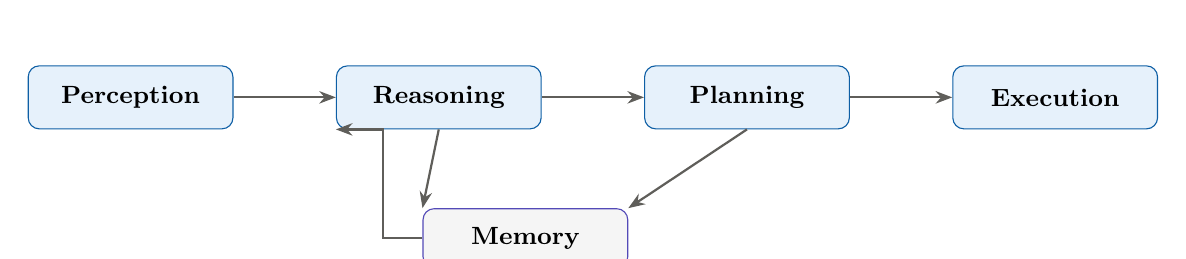
\begin{tikzpicture}[
  comp/.style={rectangle, rounded corners=4pt, draw=aiblue, fill=infobg,
               minimum width=2.6cm, minimum height=0.8cm, align=center,
               font=\small\bfseries},
  mem/.style={rectangle, rounded corners=4pt, draw=aipurple, fill=codebg,
              minimum width=2.6cm, minimum height=0.75cm, align=center,
              font=\small\bfseries},
  arr/.style={-{Stealth[length=6pt]}, thick, color=aigray},
  node distance=0.8cm and 1.4cm
]
  \node[comp] (percept) {Perception};
  \node[comp, right=1.3cm of percept] (reason)  {Reasoning};
  \node[comp, right=1.3cm of reason]  (plan)    {Planning};
  \node[comp, right=1.3cm of plan]    (exec)    {Execution};
  \node[mem,  below=1.0cm of reason, xshift=1.1cm] (mem) {Memory};

  \draw[arr] (percept) -- (reason);
  \draw[arr] (reason)  -- (plan);
  \draw[arr] (plan)    -- (exec);
  \draw[arr] (reason.south)  -- (mem.north west);
  \draw[arr] (plan.south)    -- (mem.north east);
  \draw[arr] (mem.west) -- ++(-0.5,0) |- (reason.south west);
\end{tikzpicture}
\end{center}

\begin{itemize}[leftmargin=1.5em]
  \item \textbf{Perception:} visual (CV), auditory (ASR), textual (NLP/NER),
    environmental (sensor fusion), and predictive (anticipating future states).
  \item \textbf{Reasoning:} context understanding, pattern recognition --- the LLM
    forward pass, optionally with chain-of-thought (Chapter~17).
  \item \textbf{Planning:} goal-setting, decision-making. ReAct, ReWOO, MCTS (Chapter~23).
  \item \textbf{Execution:} API calls, tool invocations, code execution (Chapter~20).
  \item \textbf{Memory:} working (context window), episodic (logs), semantic (vector DB),
    procedural (RL / fine-tuning) (Chapter~22).
\end{itemize}

\subsection{One mental model}

\begin{itemize}[leftmargin=1.5em]
    \item Pretraining gives the base capability.
    \item Fine-tuning aligns it to a job.
    \item Distillation lowers serving cost.
    \item Quantization lowers runtime footprint.
    \item RAG adds external knowledge at inference time.
    \item Agent tooling turns answers into actions.
\end{itemize}


\end{document}
